%  LaTeX support: latex@mdpi.com
%  MDPI MAKE submission — main_paper_MAKE34.tex
%  English version of main_paper_NN34.tex (Japanese draft, version 34)
%  Version 34: revisions addressing Review_codex33.txt (Major 1--8, Minor 1--10) + shortening
%    - one-sentence contribution statement + comparison table vs prior work (Major 1)
%    - summary-level mknee statements unified as "local refinement conditional on a
%      TwoNN-derived search window" (Major 2)
%    - Fashion-MNIST demoted to exploratory supplementary evidence in appendix (Major 3)
%    - stability-vs-bias distinction made more prominent (Major 4)
%    - tau_eff arguments labeled heuristic extrapolation + operational definition (Major 5)
%    - shorter abstract, reduced repetition, single-seed material moved to appendix (Major 6)
%    - stable identification framed as reporting criteria (Major 7)
%    - concrete reproducibility details (Major 8); target-vs-estimator table (Minor 2)
%  Compiled with official mdpi.cls
%  Compile: pdflatex main_paper_MAKE34.tex  (x3 for cross-references)

%=================================================================
\documentclass[make,article,submit,pdftex,moreauthors]{Definitions/mdpi}

%=================================================================
% MDPI internal commands — do not modify
\firstpage{1}
\makeatletter
\setcounter{page}{\@firstpage}
\makeatother
\pubvolume{8}
\issuenum{1}
\articlenumber{0}
\pubyear{2026}
\copyrightyear{2026}
%\externaleditor{Firstname Lastname}
\datereceived{ }
\daterevised{ }
\dateaccepted{ }
\datepublished{ }

%=================================================================
% Notation shorthands (kept in sync with main_paper_NN30.tex)
\newcommand{\dID}{d_{\mathrm{ID}}}
\newcommand{\dz}{m}
\newcommand{\dzopt}{m^{\mathrm{cand}}}
\newcommand{\dtrue}{d_{\mathrm{true}}}
\newcommand{\Jg}{J_g}
\newcommand{\R}{\mathbb{R}}
\newcommand{\kap}{\kappa}
\newcommand{\AUsat}{\mathrm{AU}_{\mathrm{sat}}}
\newcommand{\dzsat}{m^{\mathrm{sat}}}
\newcommand{\mknee}{m^{\mathrm{knee}}}
\newcommand{\demb}{d_{\mathrm{emb}}}
\newcommand{\hatdID}{\hat{d}_{\mathrm{ID}}}

%=================================================================
\Title{Diagnostic Interpretation of Effective Latent Dimensionality in
Autoencoders and Variational Autoencoders}

% ORCID IDs (replace 000X with actual ORCID or comment out)
%\newcommand{\orcidauthorA}{0000-0000-0000-000X}
%\newcommand{\orcidauthorB}{0000-0000-0000-000X}
%\newcommand{\orcidauthorC}{0000-0000-0000-000X}

\Author{Chika Obata $^{1}$,
        Mizuki Dai $^{1}$, and
        Kenya Jin'no $^{1,}$*}

\AuthorNames{Chika Obata, Mizuki Dai, and Kenya Jin'no}

\address{%
$^{1}$ \quad Department of Intelligent Systems,
  Faculty of Information Engineering,
  Tokyo City University,
  1-28-1 Tamazutsumi, Setagaya-ku, Tokyo 158-8557, Japan;
  g2332016@tcu.ac.jp (C.O.); g2591402@tcu.ac.jp (M.D.)}

\corres{Correspondence: kjinno@tcu.ac.jp; Tel.: +81-3-5707-0104 (K.J.)}

%=================================================================
\abstract{%
This paper proposes a multi-indicator diagnostic framework for interpreting
the effective latent dimensionality actually used by autoencoders (AEs) and
variational autoencoders (VAEs).
The framework distinguishes, rather than conflates, target quantities of
different natures---the number of KL-active coordinates (AU values) and the
intrinsic dimension of the latent representation (TwoNN/MLE ID)---and provides
an indicator taxonomy in which AU values serve as a robust direct observable
(``robust'' meaning low inter-seed variance under our conditions), TwoNN/MLE
ID estimates serve as numerically stable auxiliary reference estimators, and
the AU slowdown point $\mknee$ is treated as an exploratory change point.
Theoretically, under a linear-Gaussian rate--distortion surrogate (an
interpretive surrogate), we derive the activation condition
$\lambda_j > \beta\tau^2$ for the $j$-th eigendirection.
Experimentally, we confirm high multi-seed reproducibility of AU values and
TwoNN IDs for MNIST FC-VAEs, whereas $\mknee$ fluctuates strongly on sparse
$m$-grids and stabilizes at $10.3 \pm 0.9$ only as a
\textbf{local refinement conditional on a TwoNN-derived search window}
(not a validation independent of TwoNN).
Conv-VAE and natural-image experiments further quantify the boundary
conditions under which AU/$\mknee$ diagnostics become inconclusive.
Detailed scope restrictions are stated explicitly in
Section~\ref{sec:intro_structure}.}

\keyword{variational autoencoder; effective latent dimensionality;
active units; intrinsic dimension; TwoNN; diagnostic framework;
representation learning; knowledge extraction; posterior collapse}

%=================================================================
\begin{document}

\section{Introduction}\label{sec:intro}

\subsection{Background: The Problem of Interpreting Effective Latent Dimensionality}\label{sec:intro_bg}

In representation learning, autoencoders (AEs) and
variational autoencoders (VAEs)~\cite{kingma2014vae} are
core unsupervised models that learn low-dimensional latent representations
from high-dimensional data~\cite{bengio2013representation}.
The most fundamental design parameter governing the ``quality'' of these
latent representations is the bottleneck dimension~$m$:
if $m$ is too small, information is lost, whereas if it is too large,
redundant dimensions arise (and, in VAEs, posterior collapse
worsens~\cite{lucas2019elbo}).

However, a methodology for quantitatively reading ``how many dimensions a
learned latent representation actually uses''---that is, the
\textbf{effective latent dimensionality}---has not been sufficiently
established in deep representation learning research.
Existing studies~\cite{ansuini2019intrinsic,valeriani2023geometry} have
measured the intrinsic dimension of individual layers of deep networks,
but studies that systematically analyze the effective dimensionality at the
bottleneck of AEs/VAEs together with its training dynamics remain limited.

The central question addressed in this paper is:
\begin{quote}
\textit{How do AEs/VAEs ``learn'' the local intrinsic dimensionality and the
topological embedding dimensionality of the input data as the effective
dimensionality of the latent space?
And is there a way to quantitatively read this effective dimensionality
from the outside?}
\end{quote}

\subsection{Positioning and Contributions of This Study}\label{sec:intro_aim}

The central contribution of this paper can be stated in one sentence:
\begin{quote}
\textbf{The novelty of this study is not a new dimension estimator, but the
organization of known ingredients (AU values, TwoNN/MLE ID, the MSE elbow, and
PCA) into an operational taxonomy---robust indicator / auxiliary reference /
exploratory indicator---together with an empirical delineation of when each
indicator is stable and when it breaks down.}
\end{quote}
We do not claim that ``$\mknee$ uniquely identifies an appropriate
bottleneck dimension''---the primary readout of effective dimensionality is
carried by the robust indicator (AU values) and the numerically stable
auxiliary reference estimator (TwoNN ID) (Table~\ref{tab:indicator_class}).
Table~\ref{tab:novelty} positions this paper relative to prior work.

\begin{table}[H]
\caption{Positioning relative to prior work: known ingredients vs.\ contributions of this paper.}
\label{tab:novelty}
\begin{tabularx}{\textwidth}{p{3.4cm}XX}
\toprule
\textbf{Ingredient} & \textbf{Prior work} & \textbf{This paper} \\
\midrule
AU / posterior collapse & Qualitative analysis in linear VAEs \cite{lucas2019elbo} & Multi-seed reproducibility of AU$(m)$ dynamics across $m$-grids; slowdown point $\mknee$ and its instability characterization \\
TwoNN / MLE ID & Estimators \cite{facco2017twonn,levina2005mle}; measuring trained networks \cite{ansuini2019intrinsic,pope2021intrinsic} & Stability-vs-bias separation as a latent-space auxiliary reference; dominant stability condition $m \gg \hatdID$ (Exp-Real-Geom) \\
$\beta$-VAE activation & PPCA at $\beta=1$ \cite{tippingbishop1999ppca}; qualitative $\beta$ effects \cite{higgins2017betavae,lucas2019elbo} & Closed-form threshold $\lambda_j > \beta\tau^2$ under a linear-Gaussian rate--distortion surrogate (Theorem \ref{thm:linear_vae}) \\
Indicator combination & Individual indicators used in isolation & Operational taxonomy (robust / auxiliary / exploratory) with quantified validity ranges and boundary conditions \\
\bottomrule
\end{tabularx}
\end{table}

Concretely, the \textbf{contributions of this paper are threefold}:
\begin{enumerate}
  \item \textbf{A multi-indicator diagnostic framework (operational taxonomy)}:
        We distinguish AU values as a robust indicator, TwoNN ID as a numerically
        stable auxiliary reference estimator, and $\mknee$ as an exploratory
        change point (Section~\ref{sec:framework}).
        Three-seed verification on MNIST confirms the reproducibility of
        AU values ($\sigma \leq 0.5$) and TwoNN ID ($10.03 \pm 0.12$), and we
        obtain $\mknee = 10.3 \pm 0.9$ as a
        \textbf{local refinement conditional on a TwoNN-derived search window}
        (Exp-Mnist-Dense-300, Section~\ref{sec:exp_el})---not a validation
        independent of TwoNN; the verified scope is limited to MNIST FC-VAEs
        with $\beta = 4$ and three seeds.
  \item \textbf{An AU activation condition under a linear-Gaussian
        rate--distortion surrogate}:
        We derive the activation condition $\lambda_j > \beta\tau^2$ from the
        water-filling theorem and the KKT conditions
        (Theorem~\ref{thm:linear_vae}, Section~\ref{sec:theory}).
        This is not a rigorous theorem for trained non-linear VAEs but an
        interpretive surrogate providing qualitative correspondence with the
        non-linear experiments.
  \item \textbf{Quantification of the applicability range and boundary conditions}:
        We empirically demonstrate that ``$m \gg \hatdID$ is the dominant
        condition for TwoNN stability, more important than isometry improvement''
        (Exp-Real-Geom, Proposition~\ref{thm:twonn_stability}), and quantify the
        boundary conditions under which AU/$\mknee$ diagnostics become difficult
        for Conv-VAEs and natural images, as five reporting criteria
        (Sections~\ref{sec:disc_convvae} and~\ref{sec:disc_limitation}).
\end{enumerate}

\subsection{Two Kinds of ``Dimension'': Local Intrinsic Dimension and Topological Embedding Dimension}\label{sec:intro_dim}

In this paper, we distinguish two notions of manifold ``dimension'':
$\dID$ (the local intrinsic dimension, the target of TwoNN/MLE estimation) and
$\demb$ (the topological minimal embedding dimension, the minimal dimension
required for an embedding without self-intersection)
(for the Swiss Roll, $\demb = \dID = 2$; for the Torus, $\demb = 3 > \dID = 2$).

Note, however, that \textbf{the main contribution of this paper is not to prove a
correspondence with $\dID$ or $\demb$, but to organize the robustness, limits,
and applicability conditions of the diagnostic indicators AU values, TwoNN ID,
and $\mknee$}.
The conditional correspondence between $\demb$ and $\AUsat$ (for the Torus,
M\"obius strip, etc.) is positioned as an incidental supporting observation
(Section~\ref{sec:disc_incidental}).

\subsection{Research Questions}\label{sec:intro_rq}

\begin{description}
  \item[RQ1] Under what grid-density, seed-count, and architecture conditions can
             the change point $\mknee$ obtained from the AU dynamics of a VAE be
             used as a diagnostic auxiliary quantity consistent with TwoNN/MLE
             ID estimates?
  \item[RQ2] Does a framework that interprets the effective latent dimensionality
             of AEs/VAEs with multiple indicators (AU values, TwoNN/MLE, the MSE
             elbow, and PCA) provide complementary information relative to any
             single indicator?
  \item[RQ3] How do bottleneck headroom (the magnitude of $m / \hat{d}_\mathrm{ID}$)
             and geometric regularization (IsometricAE) affect the stability of
             TwoNN ID estimation?
\end{description}

\subsection{Paper Organization}\label{sec:intro_structure}

\textbf{Explicit scope of validation}:
The validation in this paper covers synthetic manifolds
($d_{\mathrm{true}} \leq 3$), MNIST and Fashion-MNIST (fully connected AE/VAE),
Conv-AE/VAE, and natural images (CIFAR-10 and SVHN).
In the natural-image experiments, we confirm that the TwoNN auxiliary estimate
yields values consistent with those reported by
Pope et al.~\cite{pope2021intrinsic}, and we quantify the validity range and
limiting conditions of AU/$\mknee$ diagnostics for Conv-VAEs
(we do not claim ``generalization'' of the entire framework to natural images).

The paper is organized as follows:
Section~\ref{sec:related} (related work), Section~\ref{sec:framework} (framework),
Section~\ref{sec:theory} (theoretical background, including Theorem~\ref{thm:linear_vae}),
Section~\ref{sec:exp} (experiments), Section~\ref{sec:discussion} (discussion),
and Section~\ref{sec:conclusion} (conclusions).
Detailed proofs and sensitivity analyses are collected in the appendices.

%% ===================================================================
\section{Related Work}\label{sec:related}

\subsection{Representation Learning and Autoencoders}\label{sec:related_ae}

Bengio et al.~\cite{bengio2013representation} organized the theoretical
framework of representation learning and discussed the mechanism by which AEs
learn the low-dimensional structure of high-dimensional data based on the
manifold hypothesis~\cite{fefferman2016manifold}.
$\beta$-VAE~\cite{higgins2017betavae} promotes disentangled representations by
increasing the KL-regularization weight $\beta$, which directly affects AU
(the linear-VAE analysis of posterior collapse is discussed in
Section~\ref{sec:related_au}).
From the perspective of score matching, the DAE analysis~\cite{alain2014dae}
showed that the reconstruction directions of denoising autoencoders selectively
suppress the normal directions of the manifold.
The CAE~\cite{rifai2011cae} learns contractive representations by regularizing
the encoder-side Jacobian.

\subsection{Intrinsic-Dimension Analysis of Deep Representations}\label{sec:related_id}

Pope et al.~\cite{pope2021intrinsic} showed via TwoNN estimation that the
intrinsic dimension of natural images is far lower than the pixel dimension
(CIFAR-10: $d_\mathrm{ID} \approx 26$ at $32 \times 32$).
Ansuini et al.~\cite{ansuini2019intrinsic} quantified the patterns by which ID
changes across the layers of deep networks, documenting contraction and
expansion phenomena of the representations.
Valeriani et al.~\cite{valeriani2023geometry} systematically analyzed the
geometric structure of the hidden representations of large transformer models.
Birdal et al.~\cite{birdal2021intrinsic} analyzed the relationship to
generalization error by integrating persistent homology with ID.
Our study is complementary to these works that ``measure the ID of existing
networks,'' and differs in that it tracks the formation of effective
dimensionality at the \textbf{design stage} and during the
\textbf{training dynamics} of AEs/VAEs.

As intrinsic-dimension estimation methods, we adopt
TwoNN~\cite{facco2017twonn} (two-nearest-neighbor distance ratios) and
MLE~\cite{levina2005mle} (maximum-likelihood estimation).
DANCo~\cite{ceruti2014danco} is more precise but computationally more expensive.
While UMAP~\cite{mcinnes2018umap} is widely used as a non-linear
dimensionality-reduction technique for visualization, our study focuses not on
visualization but on the \textbf{quantitative interpretation} of the bottleneck
dimension.

\subsection{Active Units and Posterior Collapse}\label{sec:related_au}

The active-unit (AU) count~\cite{lucas2019elbo,higgins2017betavae} is the
number of latent dimensions whose posterior-mean variance exceeds a threshold
$\delta$, and it quantifies the number of dimensions in which KL regularization
is functioning effectively.
Lucas et al.~\cite{lucas2019elbo} analyzed, within a linear-VAE framework, the
conditions under which ELBO minimization induces posterior collapse, and
qualitatively discussed the relationship between AU and the eigenvalue
structure of the data.
In contrast, our Theorem~\ref{thm:linear_vae} \textbf{quantifies Lucas et al.'s
qualitative argument as the closed-form threshold $\lambda_j > \beta\tau^2$}
in terms of the data eigenvalues $\lambda_j$, the noise $\tau^2$, and the
regularization $\beta$; its novelty lies in carrying out a quantitative
derivation under the linear-Gaussian rate--distortion surrogate, using an
explicit connection to Shannon's water-filling theorem and the KKT conditions
(it also subsumes the $\beta=1$ special case of PPCA by Tipping \&
Bishop~\cite{tippingbishop1999ppca}).
Moreover, the systematic analysis of AU growth dynamics on real data---in
particular the concept of $\mknee$ and its correspondence with effective
representational dimensionality, its limiting conditions, and stabilization
strategies---is systematically validated in this study
(Theorem~\ref{thm:linear_vae}, Proposition~\ref{thm:mknee_instab},
Section~\ref{sec:disc_mknee_improve}).

\subsection{Geometric Autoencoders}\label{sec:related_geo}

Nazari et al.~\cite{nazari2023geometric} proposed geometric autoencoders,
introducing a regularizer that makes the encoder preserve the geometric
structure of the manifold.
Kato et al.~\cite{kato2020rdae} proposed IsometricAE, which realizes an
isometric embedding by driving the pullback metric of the decoder Jacobian
toward the identity matrix.
In this study, we position IsometricAE as ``an auxiliary tool that improves a
precondition (isometry) for the readout accuracy of effective dimensionality''
(RQ3, experiment Exp-Syn-Iso).

%% ===================================================================
\section{Framework: Reading Out the Effective Latent Dimensionality}\label{sec:framework}

\subsection{Problem Setup and Main Notation}\label{sec:framework_setup}

We define an AE/VAE with input dimension $N$ and bottleneck dimension $m$:
an encoder $f: \R^N \to \R^m$ and a decoder $g: \R^m \to \R^N$.
For a VAE, the encoder outputs a posterior
$q_\phi(z|x) = \mathcal{N}(\mu(x), \sigma^2(x))$,
and the KL regularization (with strength $\beta$) acts as an information bottleneck.

\textbf{Definition of Active Units (AU)}:
\begin{equation}
  \mathrm{AU}(m) = \sum_{k=1}^{m} \mathbf{1}\bigl[\mathrm{Var}_x[\mu_k(x)] > \delta\bigr],
  \quad \delta = 10^{-2}
  \label{eq:au_def}
\end{equation}
where $\mu_k(x)$ is the $k$-th component of the posterior mean and $\delta$ is a
threshold (following Lucas et al.~\cite{lucas2019elbo}).
AU is extremely robust to this threshold choice: a sensitivity analysis confirms
that the AU values remain essentially unchanged for
$\delta \in [10^{-3}, 10^{-1}]$ (see Appendix~\ref{app:delta}).

\textbf{Definition of the AU increase rate (two steps)}:
We first define the raw increase rate $s(m_i)$ on the grid as
\begin{equation}
  s(m_i) = \frac{\mathrm{AU}(m_i) - \mathrm{AU}(m_{i-1})}{m_i - m_{i-1}}
  \label{eq:au_raw_rate}
\end{equation}
where $m_{i-1}$ is the immediately preceding value on the grid.
We then define the normalized increase rate $\rho(m_i)$ as
\begin{equation}
  \rho(m_i) = \frac{s(m_i)}{\max_j s(m_j)}
  \label{eq:au_rate}
\end{equation}
so that $\rho(m_i) \in [0, 1]$.

Table~\ref{tab:notation} lists the \textbf{main notation}.

\begin{table}[H]
\begin{adjustwidth}{-\extralength}{0cm}
\centering
\caption{Notation used throughout this paper}
\label{tab:notation}
\small
\begin{tabular}{lll}
\toprule
Symbol & Meaning & Section \\
\midrule
$m$ & Bottleneck dimension (design parameter) & §\ref{sec:framework} \\
$\dzopt$ & Diagnostic candidate dimension (not a unique optimum) & §\ref{sec:framework} \\
$\dzsat$ & AU sharp saturation point (diagnostic candidate for synthetic manifolds) & §\ref{sec:framework} \\
$\mknee$ & AU slowdown point (rough heuristic for real data) & Equation~\eqref{eq:mknee} \\
$\AUsat$ & Maximum AU value over the grid & Equation~\eqref{eq:au_def} \\
$\hat{\dID}$ & ID estimate via TwoNN/MLE & §\ref{sec:framework} \\
$\dtrue$ & True intrinsic dimension of synthetic manifold (known) & §\ref{sec:exp_synthetic} \\
$\demb$ & Topological minimum embedding dimension ($\demb \geq \dID$) & §\ref{sec:intro_dim} \\
$\kap$ & Decoder Jacobian condition number (isometry indicator) & §\ref{sec:related_geo} \\
$s(m_i)$ & Raw AU increase rate per unit dimension & Equation~\eqref{eq:au_raw_rate} \\
$\rho(m_i)$ & Normalized AU increase rate ($\in[0,1]$) & Equation~\eqref{eq:au_rate} \\
$\tau_{\mathrm{knee}}$ & Slowdown detection threshold (default: 0.25) & Equation~\eqref{eq:mknee} \\
\bottomrule
\end{tabular}
\end{adjustwidth}
\end{table}

The core of our framework is the explicit classification of each indicator as a
\textbf{robust indicator} or an \textbf{exploratory indicator}, followed by their
complementary use (Table~\ref{tab:indicator_class}).
This classification is an empirical one grounded in the experimental findings
reported later (§\ref{sec:exp_multiseed2}), and it forms the core of a design
philosophy that systematically avoids the misdiagnoses caused by overreliance on
any single indicator.

\textbf{On the meaning of ``robust indicator'' and ``exploratory indicator''}:
``Robust'' here does not mean unbiased with respect to the true intrinsic dimension.
We use the term in the sense that, at least under our experimental conditions,
the variance with respect to random seeds is small.
``Exploratory,'' in contrast, means that the indicator is useful for grid design
and hypothesis generation but is not treated as a unique estimate of the
effective latent dimensionality.

\begin{table}[H]
\begin{adjustwidth}{-\extralength}{0cm}
\centering
\caption{Classification and empirical reliability of diagnostic indicators. Throughout this paper, ``robust'' means \textit{low inter-seed variance under our experimental conditions}, not unbiasedness with respect to the true intrinsic dimension.}
\label{tab:indicator_class}
\small
\begin{tabular}{p{3.2cm}p{3.0cm}p{3.8cm}p{3.8cm}}
\toprule
Indicator & Category & Empirical reliability (inter-seed $\sigma$) & Primary use \\
\midrule
AU values ($\mathrm{AU}(m)$) & \textbf{Robust indicator} & $\sigma \leq 0.5$ (MNIST 300ep) & Direct observation of effective dimensionality; independent of reference AE geometry (depends on $\beta$, $\delta$, model capacity) \\
TwoNN ID ($\hat{d}_\mathrm{ID}$) & \textbf{Numerically stable auxiliary reference}$^\dagger$ & $\sigma \leq 0.12$ ($m=64$) & Reference estimate of intrinsic dimension \\
MSE elbow & Auxiliary indicator & Qualitative only & Reconstruction-side verification \\
PCA cumulative variance & Auxiliary indicator & Linear assumption only & Linear baseline \\
$\mknee$ (AU slowdown point) & \textbf{Exploratory indicator} & $\sigma=15$ (sparse grid); $\sigma=0.9$ (dense grid) & Rough heuristic of effective dimensionality \\
\bottomrule
\end{tabular}
\par\medskip
\footnotesize
$^\dagger$ TwoNN ID is a \textbf{supplementary reference estimator} subject to isometry bias ($\kap \approx 10^9$); see §\ref{sec:framework_pipeline} for details.
$\sigma$ of $\mknee$ is for sparse grid; improved to $\sigma=0.9$ with dense grid (Exp-Mnist-Dense), where grid design is a major factor (§\ref{sec:exp_el}).
\normalsize
\end{adjustwidth}
\end{table}

\subsubsection*{Distinguishing the Target Quantities of Each Indicator}\label{sec:framework_targets}

Under the umbrella term ``effective latent dimensionality,'' several quantities
of genuinely different nature are in fact being measured.
To avoid misdiagnosis, we explicitly distinguish five target quantities and
their estimators/observables, as summarized in Table~\ref{tab:target_estimator}.

\begin{table}[H]
\caption{Target quantities vs.\ estimators/observables. The paper's claims are stated on top of these distinctions.}
\label{tab:target_estimator}
\begin{tabularx}{\textwidth}{p{4.4cm}p{4.0cm}X}
\toprule
\textbf{Target quantity} & \textbf{Estimator / observable} & \textbf{Status} \\
\midrule
(i) Intrinsic dim.\ of the data manifold $d_\mathrm{ID}^\mathrm{data}$ & Known $\dtrue$ (synthetic); input-space TwoNN/MLE (real data) & Approximation only; no claim beyond synthetic cases \\
(ii) Intrinsic dim.\ of the latent representation $d_\mathrm{ID}^\mathrm{latent}$ & TwoNN/MLE on reference-AE latents (our $\hatdID$) & Numerically stable \textbf{latent-side reference}; may differ from (i) via embedding distortion (Section~\ref{sec:disc_twonn_bias}) \\
(iii) Number of KL-active coordinates & AU value; change point $\mknee$; maximum $\AUsat$ & Observable of coordinate usage; depends on $\beta$, $\delta$, architecture; \textbf{not} an ID estimator \\
(iv) Bottleneck dim.\ required for reconstruction & MSE elbow (qualitative) & Reconstruction-side reference \\
(v) Diagnostic candidate dimension $\dzopt$ & Designer's choice cross-checking (i)--(iv) & Not a unique optimum \\
\bottomrule
\end{tabularx}
\end{table}

The claims of this paper are stated on top of this distinction:
Theorem~\ref{thm:linear_vae} gives the threshold for (iii) in a linear surrogate;
Proposition~\ref{thm:twonn_stability} and experiment Exp-Real-Geom address the
stability conditions of (ii); and the $\mknee$ stabilization result
(Section~\ref{sec:exp_el}) identifies conditions under which the change point of
(iii) stabilizes near (ii).
We make no claims about (i) itself except for synthetic manifolds with known
$\dtrue$.

\subsection{Pipeline for Reading Out the Effective Latent Dimensionality}\label{sec:framework_pipeline}

The framework proposed in this study is an interpretation pipeline that
``reads out the effective latent dimensionality learned by an AE/VAE in two
stages'' (Figure~\ref{fig:framework}).

\textbf{Stage~1: Approximate estimation of the intrinsic dimension (auxiliary role)}

In this paper, we estimate the intrinsic dimension $\hat{d}_\mathrm{ID}$ in two ways:
(a) for \textbf{synthetic manifolds}, TwoNN/MLE is applied directly in the input
space (allowing comparison with $\dtrue$);
(b) for \textbf{real data (MNIST, etc.)}, to avoid the curse of high
dimensionality, the estimate is obtained via the latent representation of a
larger reference AE ($m_{\mathrm{ref}} = 256$).

\textbf{Explicit statement of limitations}: The latent space of the reference AE
in method (b) ($m = 256 \gg \hat{d}_\mathrm{ID}$) does not guarantee isometry
($\kap \approx 10^9$; §\ref{sec:disc_limitation}),
so the resulting $\hat{d}_\mathrm{ID}$ is an approximation that is
\textbf{numerically stable yet potentially subject to isometry bias}
(the stability-vs-accuracy distinction is discussed in
Section~\ref{sec:disc_twonn_bias}).
We treat $\hat{d}_\mathrm{ID}$ as auxiliary prior information indicating the
candidate range, and entrust the primary readout to the AU dynamics of Stage~2.
Practical stability is ensured by confirming that the estimates converge across
multiple values of $m$ (e.g., $\{64, 128, 256\}$).

\textbf{Stage~2: Reading out the effective dimensionality via AU dynamics}

We sweep the bottleneck dimension $m$ over the discrete grid
$\mathcal{M} = \{1, 2, 4, 8, 12,\allowbreak 16, 20, 32,\allowbreak 64, 128, 256\}$,
training a VAE ($\beta = 4$) at each $m$ and computing $\mathrm{AU}(m)$
(some experiments use extended grids that omit or add some of the $m$ points of
$\mathcal{M}$; these are stated explicitly in each experiment section).
Depending on the AU pattern, we read the diagnostic candidate dimension
$\dzopt$ in one of two ways
(\textbf{$\dzopt$ is not the unique ``optimal'' bottleneck dimension but a
diagnostic candidate dimension based on multiple indicators}):

\begin{description}
  \item[Saturation type (simple data such as synthetic manifolds)]
        When AU saturates sharply at a specific $m$, we use that saturation point
        $\dzsat$ as the diagnostic candidate dimension $\dzopt = \dzsat$
        (since AU values are robust, this is quite reliable under these
        conditions).
  \item[Gradual-increase type (real data, e.g., MNIST)]
        When AU increases gradually with $m$, we refer to the slowdown point
        $\mknee$ as a rough design guideline (an exploratory indicator):
        \begin{equation}
          \mknee = \min\{m_i \in \mathcal{M} : \rho(m_i) < \tau_{\mathrm{knee}}\}
          \label{eq:mknee}
        \end{equation}
        with $\tau_{\mathrm{knee}} = 0.25$ (default; see Appendix~\ref{app:tau_knee}).
        $\mknee$ roughly captures ``the point at which the VAE first performs
        significant dimensional compression,'' but its value depends on the $m$
        grid and on the random seed, so the final judgment is made by
        cross-checking against the AU values and the TwoNN ID
        (§\ref{sec:disc_mknee}).
        Even if $\mknee$ and $\hat{d}_\mathrm{ID}$ do not agree, the framework as a
        whole is not invalidated.
\end{description}

CKA~\cite{kornblith2019cka} and the reconstruction-error (MSE) elbow serve as
auxiliary criteria, and the overall judgment is made from multiple indicators.
The MSE elbow is a qualitative visual reference on the MSE$(m)$ curve;
\textbf{we do not propose an algorithmic elbow detector}
(item (iv) of Table~\ref{tab:target_estimator}).

\begin{figure}[H]
\centering
\renewcommand{\arraystretch}{1.4}
\begin{tabular}{c}
  \fbox{\textbf{Input data} $\boldsymbol{X} \in \R^N$ (under the manifold hypothesis)} \\[3pt]
  $\Big\downarrow$ \\[1pt]
  \fbox{\parbox{0.70\linewidth}{\centering
    \textbf{Stage~1: Approximate estimation of the effective intrinsic dimension}\\[1pt]
    Benchmark on synthetic manifolds (known $\dtrue$) $\to$ select TwoNN/MLE\\
    Real data: apply TwoNN/MLE to the latent representation of a reference AE ($m_{\mathrm{ref}} = 256$)\\
    $\Rightarrow$ estimate $\hat{\dID}$ (guide to the candidate range; approximate value)
  }} \\[3pt]
  $\Big\downarrow$ \\[1pt]
  \fbox{\parbox{0.70\linewidth}{\centering
    \textbf{Stage~2: Diagnosis of the effective dimensionality via AU dynamics}\\[1pt]
    Sweep VAEs over the grid $\mathcal{M}$ $\to$ track $\mathrm{AU}(m)$\\
    Saturation type: diagnostic candidate $\dzopt = \dzsat$ (highly reliable); gradual-increase type: rough guideline $\dzopt = \mknee$ (exploratory)\\
    \textbf{Primary indicators}: AU values (robust indicator), TwoNN ID (numerically stable auxiliary reference)\\
    \textbf{$\mknee$ is an exploratory guideline, not a unique optimum}
  }} \\[3pt]
  $\Big\downarrow$ \\[1pt]
  \fbox{\parbox{0.70\linewidth}{\centering
    \textbf{Auxiliary (RQ3): Verifying geometric regularization, bottleneck margin, and TwoNN stability}\\[1pt]
    Check the condition $m \gg \hat{d}_\mathrm{ID}$ $\to$ evaluate the validity range of the TwoNN auxiliary estimate
  }}
\end{tabular}
\caption{Diagnostic pipeline for effective latent dimensionality. The diagnostic candidate dimension $\dzopt$ is not a unique optimal solution but a candidate based on multiple indicators (AU values, TwoNN ID, $\mknee$).}
\label{fig:framework}
\end{figure}

\subsection{Interpretive Significance of $\mknee$}\label{sec:framework_mknee_interp}

The KL regularization deactivates surplus latent dimensions that are not needed
for reconstruction (i.e., it induces posterior collapse)
\cite{lucas2019elbo,higgins2017betavae}.
In the regime $m < \hat{d}_\mathrm{ID}$, all dimensions are activated
($\mathrm{AU}(m) \approx m$); once $m$ exceeds roughly $\hat{d}_\mathrm{ID}$,
KL pressure on the surplus dimensions slows the AU increase rate---$\mknee$ is
the change point that coarsely captures this slowdown.
Its numerical reproducibility, however, depends on the $m$ grid and on random
seeds and is not guaranteed (§\ref{sec:exp_multiseed2}, §\ref{sec:disc_mknee}).
Regardless of whether $\mknee$ agrees, the readout through the combination of AU
values and the TwoNN ID constitutes the core of this framework.

\subsection{Reporting Criteria for Stable Identification}\label{sec:natimg_stable_id}

We define here, ahead of the experiments, the criteria required to report that
AU/$\mknee$ has been ``stably identified'' on a new dataset or architecture.
These are not generally valid criteria for stable identification, but
\textbf{reporting criteria internal to this study}, calibrated from the behavior
of MNIST FC-VAEs.
In this paper, we say that \textbf{stable identification} holds when all five of
the following conditions are met:

\begin{enumerate}
  \item \textbf{Seed stability}: over 3--5 seeds, the standard deviation of
        $\mknee$ satisfies $\sigma_\mathrm{seed} \leq 0.1 \cdot \mknee$.
  \item \textbf{Grid stability}: doubling the grid density changes $\mknee$ by
        at most $20\%$.
  \item \textbf{$\beta$ stability}: changing $\beta_{\max}$ by $\pm 20\%$ keeps
        $\mknee$ within the same grid cell.
  \item \textbf{AU-plateau stability}: the across-seed standard deviation of the AU
        plateau value satisfies $\sigma \leq 0.05 \cdot \AUsat$.
  \item \textbf{TwoNN--AU consistency}: $\mknee \leq 3 \hat{d}_\mathrm{ID}$
        (coarse agreement between TwoNN and AU).
\end{enumerate}

These thresholds ($0.1\cdot\mknee$, $20\%$, $0.05\cdot\AUsat$,
$3\hat{d}_\mathrm{ID}$) are not theoretically derived universal constants but
\textbf{author-defined reporting criteria}; we make no claim that they are
meaningful as general standards beyond this study.
The numerical choices take the scale of the across-seed variability observed for
MNIST FC-VAEs (AU: $\sigma \leq 0.5$; dense-grid $\mknee$:
$\sigma = 0.9 \approx 0.09\,\mknee$; Section~\ref{sec:exp_el}) as the yardstick
for ``stable,'' rounded so that variability exceeding it by orders of magnitude is
judged ``unstable.''
A systematic sensitivity analysis of the thresholds themselves is left as future
work, but the conclusion of this paper (none of the five criteria are met for
natural images; Section~\ref{sec:exp_natimg_sweep}) is clear-cut enough that it
does not change even if the thresholds are relaxed by a factor of two.
The purpose of the criteria is not to declare ``success'' but to decompose and
report \textbf{which conditions are violated} when stable identification is not
achieved.

%% ===================================================================
\section{Theoretical Background}\label{sec:theory}

In this section, we present the theoretical foundations that support the framework.
Proposition~\ref{thm:lower_bound} is a lower bound based on standard topological facts
about topological dimension and embedding dimension; its rigorous claim is restricted to
the idealized premise of ``the dimension required to achieve zero reconstruction error.''
\textbf{Theorem~\ref{thm:linear_vae}} is an analytical result under the linear-Gaussian
rate--distortion surrogate and gives the AU activation threshold in closed form
(proof details in~\ref{app:proofs}).
Proposition~\ref{thm:mknee_instab} is a lemma under an idealized monotone-saturation model;
note that in practical non-linear settings, errors exceeding the upper bound can occur.
Proposition~\ref{thm:twonn_stability} is not a guarantee of unbiasedness but a sketch of
sufficient conditions for conditional stability.
Proposition~\ref{thm:pullback} follows directly from the definition of isometry.

\begin{Proposition}[Topological Lower Bound on the Bottleneck Dimension]\label{thm:lower_bound}
For a smooth $d$-dimensional manifold $\mathcal{M} \subset \R^N$ to be reconstructed by
a continuous AE without self-intersection, ideally achieving zero reconstruction error,
a bottleneck dimension $m \geq d$ is necessary.
(Practical settings involving finite samples, finite capacity, and approximate
reconstruction are outside the scope of this idealization.)
\end{Proposition}

\begin{proof}
Zero reconstruction error requires $g \circ f|_\mathcal{M}$ to be close to the identity map,
so $f|_\mathcal{M}: \mathcal{M} \to \R^m$ must be a continuous injection.
By standard properties of the topological embedding dimension
(Hatcher~\cite{hatcher2002algebraic}, Chapter~2), no continuous injection exists from a
$d$-dimensional manifold into a Euclidean space of dimension $m < d$;
hence $m \geq d$ is a necessary condition.
\end{proof}

This proposition justifies $\hat{d}_\mathrm{ID}$ as a reference point for a principled
lower bound on the bottleneck dimension
(in practice, we use it as a ``candidate range for the effective dimensionality'').
Experiment Exp-Syn-1 confirms this: at the transition $m = 1 \to 2$, the MSE improves by
roughly a factor of 35 on the Swiss Roll (Section~\ref{sec:exp_synthetic}).

%% ─── Theorem 1: AU saturation threshold of the linear β-VAE ────────────────
\begin{Remark}[Relation to Prior Work]
Our theorem is closely related to a family of known analyses---the discussion of
posterior collapse in linear VAEs by Lucas et al.~\cite{lucas2019elbo},
probabilistic PCA by Tipping \& Bishop~\cite{tippingbishop1999ppca}
(corresponding to the special case $\beta = 1$), and Shannon's water-filling
theorem~\cite{cover2006elements}---and its novelty is limited to organizing these
into a closed-form threshold $\lambda_j > \beta\tau^2$ for the $\beta$-ELBO with
$\beta \neq 1$, together with monotone saturation.
The role of the theorem is not to present a new mathematical result, but to
provide a quantitative reference point for interpreting the non-linear
experiments.
\end{Remark}

\begin{Theorem}[AU Activation Threshold under the Linear-Gaussian Rate--Distortion Surrogate]\label{thm:linear_vae}
For a $\beta$-VAE with linear encoder, linear decoder, and Gaussian prior
(detailed setting in~\ref{app:proofs}),
\textbf{under the linear-Gaussian rate--distortion surrogate},
the water-filling theorem and the KKT conditions yield the following:

\begin{enumerate}
  \item \textbf{(Activation threshold)} The $j$-th eigen-direction becomes active iff
        \begin{equation}
          \lambda_j > \beta \tau^2 \label{eq:au_threshold}
        \end{equation}
        where $\lambda_j$ is the \textbf{$j$-th eigenvalue of the covariance matrix of
        the centered input data},
        $\Sigma = \mathbb{E}[(x-\bar{x})(x-\bar{x})^\top]$
        (i.e., the variance of the $j$-th principal component in the input-space PCA
        basis), and $\tau^2$ is the isotropic Gaussian observation-noise variance of
        the decoder output.
  \item \textbf{(Upper bound on the optimal number of active eigen-directions)}
        The number of active eigen-directions at the global optimum, $A^*(m)$,
        satisfies $A^*(m) \leq \min\bigl(m,\; d^*(\beta)\bigr)$, where
        $d^*(\beta) := \bigl|\{j : \lambda_j > \beta\tau^2\}\bigr|$.
  \item \textbf{(Monotone saturation at the optimum)}
        $A^*(m)$ is monotone non-decreasing in $m$ and saturates for
        $m \geq d^*(\beta)$ (i.e., $A^*(m) = d^*(\beta)$).
\end{enumerate}

\noindent
A detailed derivation is given in~\ref{app:linear_vae_proof}.
The quantity $\beta\tau^2$ acts as the ``water level'' of water-filling:
only eigen-directions whose eigenvalues exceed it become active.
This theorem is not a theorem about trained non-linear VAEs; it is an
\textbf{interpretive surrogate} for interpreting the non-linear experiments.
\end{Theorem}

\begin{Remark}[Relation to Empirical AU]
Item (3) of Theorem~\ref{thm:linear_vae} establishes the monotonicity of the number of
active eigen-directions $A^*(m)$ at the global optimum.
In contrast, practical non-linear VAEs are trained independently for each $m$ by
stochastic optimization, so the observed empirical AU$(m)$ can be
\textbf{non-monotone} due to finite-sample effects, initialization dependence, and
optimization noise
(e.g., in Table~\ref{tab:e4_vae}, AU$=26$ at $m=128$ falls below AU$=29$ at $m=64$).
Therefore, the empirical $\mknee$ must be treated not as a rigorous estimate of the
saturation point of $A^*$, but as an exploratory diagnostic indicator derived from the
shape of the AU curve.
\end{Remark}

\begin{proof}[Proof sketch (details in~\ref{app:proofs})]
Analyzing the $\beta$-ELBO contribution of each PCA direction $j$ independently
(a standard result for linear-Gaussian models), the ELBO gain $\Delta L_j$ from
activating direction $j$ is positive only when $\lambda_j > \beta\tau^2$
(the correspondence with Shannon's water-filling theorem).
By the independence across dimensions, the relation between the optimal AU count and
$d^*(\beta)$, as well as the monotone saturation, follows.
\end{proof}

\begin{Remark}
Implications: (i) raising $\beta\tau^2$ (stronger regularization or larger noise)
reduces the number of active dimensions.
(ii) A vanilla AE corresponds to the limit $\beta = 0$, where the threshold
vanishes, so the number of utilized latent coordinates approaches $m$
(consistent with experiment Exp-Syn-AU; Section~\ref{sec:exp_synthetic}).
(iii) As a qualitative extension to real data, the theorem provides the rule of
thumb that ``dimensions whose effective SNR falls below $\beta$ are compressed.''
\end{Remark}

%% ─── Proposition: grid sensitivity of mknee (under the idealized model) ─────
\begin{Proposition}[Grid-Resolution Dependence of $\mknee$ under the Idealized Monotone-Saturation Model]\label{thm:mknee_instab}
Assume the idealized model in which AU$(m)$ saturates ideally and monotonically at
$d^*(\beta)$ (changing in a step-like manner, with no stochastic noise).
Then, for $\mknee(\mathcal{G})$ on a grid $\mathcal{G} = \{m_1 < \cdots < m_K\}$,
\begin{equation}
  \bigl|\mknee(\mathcal{G}) - d^*(\beta)\bigr|
  \leq \max_{i} (m_{i+1} - m_i)
  \label{eq:mknee_error}
\end{equation}
holds (the error is bounded above by the maximum grid spacing).

\noindent\textit{Caution: in practical non-linear VAEs this idealization does not hold,
and shape noise in AU$(m)$ due to stochastic optimization can produce errors that
substantially exceed the upper bound in Equation~\eqref{eq:mknee_error}
(consistent with the observations in Section~\ref{sec:exp_multiseed2}).
This proposition should be treated not as a general instability theorem but as a lemma
providing guidance for grid design.}
\end{Proposition}

\begin{proof}
In the idealized monotone-saturation model, AU$(m)$ changes step-wise at $d^*(\beta)$,
so if $d^*(\beta) \in [m_{i_0}, m_{i_0+1})$, then $\mknee$ is detected as
$m_{i_0+1}$ (or $m_{i_0}$).
The error is $\leq m_{i_0+1} - m_{i_0} \leq \max_i(m_{i+1}-m_i)$.
\end{proof}

\begin{Remark}
Experimental implication of this proposition: the grid $\{4,8,12,16,20,32,64\}$ contains
a maximum spacing of 32 (from 32 to 64), so for $d^* \approx 10$ a large error with
$\mknee \in \{32, 64\}$ can arise (consistent with Section~\ref{sec:exp_multiseed2}).
A dense grid combined with a multi-seed ensemble is a practical stabilization strategy
(Section~\ref{sec:disc_mknee_improve}).
\end{Remark}

%% ─── Proposition 3: pullback metric ─────────────────────────────────────────
\begin{Proposition}[Pullback Metric and Local Isometry]\label{thm:pullback}
A necessary and sufficient condition for the decoder $g: \R^m \to \R^N$ to be locally
isometric in a neighborhood of a point $z$ is that the pullback metric satisfies
$G(z) = \Jg(z)^\top \Jg(z) = I_m$.
That is, $\|\Jg(z)dz\|^2 = \|dz\|^2$ holding for every infinitesimal displacement $dz$
is equivalent to $G(z)=I_m$ (all singular values equal to 1).

By contrast, the condition number $\kap(z) = \sigma_{\max}(\Jg) / \sigma_{\min}(\Jg)$
is an indicator of the anisotropy of the local map: $\kap = 1$ means that all singular
values are \textbf{equal} (isotropic scaling), but does not guarantee that this scale
equals 1.
For example, if $\Jg$ magnifies all directions by a factor of 2, then $\kap=1$ but the
map is not isometric.
Accordingly, in this paper we use $\kap$ not as isometry itself but as an auxiliary
indicator of local anisotropy.
\end{Proposition}

\begin{proof}
By the definition of isometry, $\|J_g dz\|^2 = \|dz\|^2$ for every $dz \in \R^m$ is
equivalent to $J_g^\top J_g = I_m$ (all singular values equal to 1).
Since $\kap = 1$ only means that all singular values are equal, whether their value is 1
is a separate matter; hence $\kap=1$ is not a necessary and sufficient condition for
isometry (see the example above).
\end{proof}

This proposition explains why an isometry bias arises in ID estimation using a reference
AE (Section~\ref{sec:disc_limitation}) and motivates the IsometricAE
(experiment Exp-Syn-Iso).

The remaining interpretive propositions (effective rank of the decoder Jacobian,
noise-direction selectivity, and neighborhood-structure preservation) are given
in~\ref{app:proofs}.

%% ─── §4.4: qualitative correspondence between linear theory and non-linear experiments (bridging note) ─────────────
\subsection{Qualitative Correspondence between Linear Theory and Non-Linear Experiments}\label{sec:theory_bridge}

Theorem~\ref{thm:linear_vae} (the water-filling principle) holds under the
linear-Gaussian rate--distortion surrogate.
In non-linear settings, a powerful decoder achieves an effective noise variance
$\tau^2_\mathrm{eff} \ll 1$, so
$d^*(\beta) = |\{j : \lambda_j > \beta\tau^2_\mathrm{eff}\}|$ becomes substantially
larger than the prediction under the linear assumption ($\tau^2=1$).
Moreover, the smooth AU growth curves produced by non-linear optimization replace the
step-like saturation transition of the linear setting, causing the instability of
$\mknee$ on sparse grids.

\textbf{Operational definition and status of $\tau^2_\mathrm{eff}$}:
Our $\tau^2_\mathrm{eff}$ is not an independently measured physical quantity;
we define it operationally as ``the calibrated value back-computed so that
$d^*(\beta) = |\{j : \lambda_j > \beta\tau^2_\mathrm{eff}\}|$, evaluated on the
input PCA spectrum $\{\lambda_j\}$, matches the observed effective
dimensionality (TwoNN ID or AU saturation value)''
($\tau^2_\mathrm{eff} \approx 0.30$ for MNIST FC-VAEs; Section~\ref{sec:exp_em}).
Consequently, arguments that extend the theorem to non-linear and convolutional
settings via $\tau^2_\mathrm{eff}$ (Section~\ref{sec:disc_convvae}) are
\textbf{heuristic extrapolations}, not consequences of the theorem; their
validity is supported only by post-hoc consistency (e.g., the qualitative
prediction that increasing $\beta$ shifts saturation to lower dimensions).

We demonstrate this qualitative inheritance (AU monotonicity, slowdown of growth beyond
the effective dimensionality) and the quantitative divergence through a MNIST PCA
spectrum analysis (experiment Exp-Mnist-PCA) in Section~\ref{sec:exp_em}.

%% ─── §4.5: conditional stability proposition for TwoNN ─────────────────────
\subsection{Conditional Stability of TwoNN: Theoretical Formulation}\label{sec:theory_stability}

In this section, motivated by the experimental observations of
Section~\ref{sec:exp_ep} (Exp-Stab, Exp-Geom, and Exp-Iso-ID),
we theoretically support, as an explanatory proposition, the question
``under what conditions can TwoNN be used as an auxiliary reference estimator?''
\textbf{This proposition does not guarantee the unbiasedness of TwoNN;
it is an interpretive proposition giving a sketch of sufficient conditions for
conditional stability}
(positioned not as a mathematically rigorous theorem but as a theoretical rationale for
a design guideline).

\begin{Proposition}[Conditional Stability of TwoNN]\label{thm:twonn_stability}
Suppose the encoder $f: \R^N \to \R^m$ is locally bi-Lipschitz,
i.e., in a neighborhood $U$ of every point $z$,
\begin{equation}
  (1-\varepsilon)\|v\| \leq \|J_f \cdot v\| \leq (1+\varepsilon)\|v\|,
  \quad \varepsilon \in [0,1)
  \label{eq:bilip}
\end{equation}
holds, and suppose further that nearest-neighbor ranks are preserved with high
probability (Trustworthiness $\geq 1 - \delta_T$ with small $\delta_T$).
Then the change in the empirical distribution of the two-nearest-neighbor distance ratio
$r_2/r_1$, measured by the earth mover's distance (EMD), is bounded as
\begin{equation}
  \mathrm{EMD}\bigl(P_{r_2/r_1}^{(\mathrm{input})},\; P_{r_2/r_1}^{(\mathrm{latent})}\bigr)
  \leq C\bigl(\varepsilon,\, \delta_T\bigr)
  \label{eq:twonn_stab}
\end{equation}
and consequently the deviation of the TwoNN estimate,
$|\hat{d}_\mathrm{ID}^{(\mathrm{latent})} - \hat{d}_\mathrm{ID}^{(\mathrm{input})}|$,
is also bounded above by a constant governed by $C(\varepsilon,\delta_T)$.
($C(\varepsilon, \delta_T) \to 0$ as $\varepsilon \to 0$ and $\delta_T \to 0$.)
\end{Proposition}

\begin{proof}
\textit{Proof sketch}:
By Equation~\eqref{eq:bilip}, the change factor of distances $d(x_i, x_j)$ lies within
the range $(1-\varepsilon)^2$ to $(1+\varepsilon)^2$.
Since the distance ratio $r_2/r_1$ is a ratio rather than an absolute distance, uniform
scale deformations (global rescaling) cancel out, but the non-isometric component with
$\varepsilon \neq 0$ alters the ratio.
Trustworthiness $\geq 1-\delta_T$ guarantees that ``the two nearest neighbors in latent
space coincide with those in input space with high probability,'' probabilistically
suppressing large fluctuations of $r_2/r_1$ caused by rank reversals.
Under these two conditions, the change in the distribution of $r_2/r_1$ is bounded above
by a continuous function $C(\varepsilon,\delta_T)$ of $\varepsilon$ and $\delta_T$
($C=0$ when $\varepsilon=0$ and $\delta_T=0$, coinciding with the isometric,
perfectly neighbor-preserving case).
\textit{(This is a finite-sample, finite-dimensional approximation; a rigorous bound
depends on the specific setting of the isometry constants.)}
\end{proof}

\begin{Remark}[Experimental Implications of Proposition~\ref{thm:twonn_stability}]
This proposition suggests that ``isometry $\varepsilon \approx 0$ is the sole condition
for TwoNN accuracy'' is not the case; rather, ``the improvement of Trustworthiness
(preservation of neighbor ranks) induced by $m \gg d_\mathrm{ID}$ may be the dominant
factor for stability.''
In experiment Exp-Stab (Section~\ref{sec:exp_ep}), the difference in TwoNN ID remained
within $\pm 2.3\%$ over the range $\kap \in [1.06, 2.16]$, whereas TwoNN recovered upon
moving from $m = d_\mathrm{true}$ to $m > d_\mathrm{true}$---consistent with the
decrease in $\delta_T$ (the neighbor-reversal rate) being more dominant than the change
in $\varepsilon$ (isometry).
This proposition does not claim that TwoNN is an ``unbiased estimator of the true
$d_\mathrm{ID}$''; it theoretically supports ``under what conditions TwoNN can be operated
as an auxiliary reference estimator.''
Experiment Exp-Real-Geom (Section~\ref{sec:exp_real_geom}) directly validates this
implication on real data.
\end{Remark}

%% ===================================================================
\section{Experiments}\label{sec:exp}

\textbf{Three-tier classification of experiments}:
The experiments in this paper are clearly classified into the following three tiers
(a complete per-experiment list of configurations and roles is given in
Table~\ref{tab:exp_full}, Appendix~\ref{app:exp_table}).
\begin{description}
  \item[\textbf{Main experiments}]
        Empirical validation of the framework core:
        Exp-Syn-1, Exp-Syn-AU, Exp-Mnist-Base, Exp-Mnist-Multi, Exp-Mnist-Dense, Exp-Real-Geom, and Exp-Nat-Cifar.
        Their primary validation targets are the robustness of AU values and TwoNN ID (RQ2) and the stabilization conditions of $\mknee$ (RQ1).
  \item[\textbf{Supplementary experiments}]
        Verification of prerequisites and interpretive claims of the main experiments:
        Exp-Stab, Exp-Geom, Exp-Iso-ID, Exp-Syn-Iso, Exp-Conv-AE, Exp-Syn-Top, Exp-Mnist-PCA, Exp-Mnist-Dyn, Exp-Mnist-Ent,
        and Exp-Fashion (exploratory; Appendix~\ref{app:fashion}).
        These verify TwoNN numerical stability, IsometricAE isometry, the theory--experiment bridge, and related points (supporting evidence for the main claims).
  \item[\textbf{Boundary experiments}]
        Quantification of the applicable range and boundary conditions:
        Exp-Conv-Fix, Exp-Conv-Ann, Exp-Conv-M256, Exp-Conv-M512, Exp-ConvV-HiBeta, Exp-NatImg-AU, Exp-NatImg-Sweep, and Exp-NatImg-Knee.
        These quantify the conditions under which stable identification of AU/$\mknee$ becomes difficult for Conv-VAEs and natural images,
        thereby establishing the validity range and the applicability boundary of the framework.
\end{description}

\subsection{Experimental Setup}\label{sec:exp_setup}

\textbf{Common settings}: Adam ($\mathrm{lr} = 10^{-3}$), batch size 128, ReLU activations (Sigmoid output layer), random seed 42, PyTorch~2.0.

\textbf{Synthetic manifolds}: hidden layers $[64, 32]$, 200--300 epochs, VAE $\beta = 4.0$, $n = 5{,}000$ (4,000 training / 1,000 test).

\textbf{MNIST / Fashion-MNIST}: input dimension 784, hidden layers $[512, 256]$, VAE $\beta = 4.0$,
grid $\mathcal{M} = \{1,2,4,8,12,16,20,32,64,128,256\}$, batch size 128.
MNIST is trained for 300 epochs ($n_{\mathrm{train}} = 20{,}000$, $n_{\mathrm{test}} = 3{,}000$),
and Fashion-MNIST for 100 epochs ($n_{\mathrm{train}} = 10{,}000$, $n_{\mathrm{test}} = 2{,}000$).

ID estimation: TwoNN ($k=2$; by the definition of the algorithm, $k=2$ is the only possible choice) and MLE ($k=10$; near the center of the range $k=5$--20 recommended by Levina \& Bickel~\cite{levina2005mle}, with stability also confirmed for $k=5,10,20$)~\cite{facco2017twonn,levina2005mle}.
AU threshold $\delta = 10^{-2}$~\cite{lucas2019elbo} (AU is extremely robust to this threshold choice: a sensitivity analysis confirmed that AU values remain essentially unchanged as $\delta$ varies over $[10^{-3}, 10^{-1}]$; Appendix~\ref{app:delta}).

\textbf{Computational environment and reproducibility}:
All experiments were run on a Linux workstation with a single NVIDIA GeForce
RTX~3070 GPU (PyTorch~2.0, CUDA~11.x; falling back to CPU when CUDA is unavailable).
Preprocessing consists solely of normalizing pixel values to $[0,1]$, with no
data augmentation (synthetic manifolds are standardized to zero mean and unit
variance).
Training and test subsets are the first $n_\mathrm{train}$ and $n_\mathrm{test}$
samples of each dataset's official train/test split in fixed order (shuffling
affects only the mini-batch order during training and is fixed by the seed).
Optimization uses Adam ($\mathrm{lr} = 10^{-3}$, $\beta_1 = 0.9$,
$\beta_2 = 0.999$, no weight decay) with batch size 128 throughout.
The bulk of the computational cost is the repetition of training runs over the
$m$ grid $\times$ seeds; a major multi-seed sweep (e.g., MNIST FC-VAE with 7--17
grid points $\times$ 3 seeds $\times$ 300 epochs) takes several hours to about a
day in this environment, and the full set of experiments amounts to several days
of GPU time.
Experiment code, configuration files, random seeds, trained-model logs (JSON),
and figure/table regeneration scripts will be provided in a public repository
(URL and archival DOI to be finalized upon acceptance; the complete code and raw
logs are attached as supplementary material for review).
A complete list of experimental configurations (dataset, model, epochs, $\beta$
schedule, $m$ grid, number of seeds, sample size, and role) is given in
Table~\ref{tab:exp_full} of Appendix~\ref{app:exp_table}, and
\textbf{single-seed results are also marked as such in the captions of the
corresponding tables and figures in the main text}.

\subsection{Synthetic Manifold Experiments: Principle Verification (RQ1, RQ2, RQ3)}\label{sec:exp_synthetic}

Using synthetic manifolds with known $\dtrue$, we verify the fundamental validity of the proposed framework.

\subsubsection{Correspondence Between MSE Elbows and Intrinsic Dimension (Experiment Exp-Syn-1)}

For the Swiss Roll ($\dtrue = 2$, simply connected) and the Torus ($\dtrue = 2$, $\demb = 3$),
we confirmed that the AE reconstruction MSE improves sharply at $m = \dtrue$ (Swiss Roll) or $m = \demb$ (Torus)
(Table~\ref{tab:e1}).

\begin{table}[H]
\centering
\caption{Exp-Syn-1: MSE of AE on synthetic manifolds (mean$\pm$std over 3 seeds).}
\label{tab:e1}
\small
\begin{tabular}{rcc}
\toprule
$m$ & Swiss Roll MSE & Torus MSE \\
\midrule
1 & $1.016\pm0.315$ & $0.356\pm0.022$ \\
2 & $\boldsymbol{0.029\pm0.001}$ $\leftarrow$ elbow & $0.109\pm0.007$ \\
3 & $(6\pm2)\times10^{-4}$ & $\boldsymbol{(4\pm3)\times10^{-4}}$ $\leftarrow$ elbow \\
4 & $(5\pm1)\times10^{-4}$ & $(1.0\pm0.4)\times10^{-4}$ \\
\bottomrule
\end{tabular}
\end{table}

For the Swiss Roll, the MSE improves by a factor of approximately 35 from $m = 1$ to $m = 2$,
experimentally confirming Proposition~\ref{thm:lower_bound}.
For the Torus, the elbow appears at $m = 3$ ($= \demb$),
showing that perfect reconstruction is impossible at $\dID = 2$.

\subsubsection{AU Saturation and Topological Structure (Experiments Exp-Syn-AU and Exp-Syn-Top)}

We compared the AU pattern of the VAE ($\beta = 4$) with that of a vanilla AE (Table~\ref{tab:ea_summary}).
\textbf{Caveat}: the ``AU'' reported for the AE in the table is a pseudo-AU defined by
whether the encoding variance of each latent coordinate exceeds $\delta$
(AU is not natively defined for AEs, which lack KL regularization); it is an
auxiliary observation.

\begin{table}[H]
\centering
\caption{Exp-Syn-AU: VAE active units (AU) for Swiss Roll (upper) and Torus (lower) (mean$\pm$std, 3 seeds).}
\label{tab:ea_summary}
\small
\begin{tabular}{rccc}
\toprule
 & $m$ & Vanilla AE (AU) & VAE (AU, $\beta=4$) \\
\midrule
Swiss Roll & 2 & 2 & $2.0\pm0.0$ \textbf{(saturation)} \\
($d_\mathrm{true}=2$) & 4 & 4 & $2.0\pm0.0$ \\
 & 8 & 8 & $2.0\pm0.0$ \\
 & 16 & 16 & $2.0\pm0.0$ \\
\midrule
Torus & 4 & 4 & $2.0\pm0.0$ \\
($d_\mathrm{true}=2$, $d_\mathrm{emb}=3$) & 6 & 6 & $3.0\pm0.0$ \textbf{(saturation)} \\
 & 8 & 8 & $3.0\pm0.0$ \\
 & 16 & 16 & $3.0\pm0.0$ \\
\bottomrule
\end{tabular}
\end{table}

Whereas the vanilla AE exhibits AU $= m$ (no saturation),
the VAE saturates at $\AUsat = 2$ ($= \dtrue$) for the Swiss Roll
and at $\AUsat = 3$ ($= \demb > \dID$) for the Torus (standard deviation 0.0 across all 3 seeds).
This is consistent with the qualitative implication of Theorem~\ref{thm:linear_vae}
(the water-filling AU saturation mechanism),
and suggests that on the Torus the KL regularization may begin compressing near the topological embedding dimension
(an empirical observation under the conditions of this study; note that this finding is preprocessing-dependent and conditional).

In experiment Exp-Syn-Top (correspondence between $\AUsat$ and $\demb$ on
topological manifolds; a single-seed incidental observation), we observed
$\AUsat = 3 = \demb$ for the Torus and the M\"obius Band (both $\dID = 2$,
$\demb = 3$), and $\AUsat = 2$ for the Circle $S^1$ ($\demb = 2$; $m \geq 6$,
conditional) (result table in Appendix~\ref{app:fashion},
Table~\ref{tab:eb_summary}).
Because the $\AUsat$ of the Swiss Roll is strongly preprocessing-dependent
(2 under standardized conditions, 3 under other conditions), we restrict the
main evidence supporting the correspondence between $\AUsat$ and $\demb$ to the
Torus and the M\"obius Band.
This correspondence is an empirical observation that depends on our experimental
conditions (standardized preprocessing, $\beta = 4$, sufficient convergence) and
is not guaranteed as a theoretical necessity (incidental finding;
\S\ref{sec:disc_incidental}).

\subsubsection{Achieving Isometry with IsometricAE (Experiment Exp-Syn-Iso)}

On the Swiss Roll ($m = 2$), we compared the isometry of four model types (Table~\ref{tab:ec}).

\begin{table}[H]
\centering
\caption{Exp-Syn-Iso: Comparison of four models on Swiss Roll ($m=2$) (mean$\pm$std, 3 seeds).}
\label{tab:ec}
\small
\begin{tabular}{lrrr}
\toprule
Model & MSE & $\kap$ & NSR \\
\midrule
AE & $0.030\pm0.003$ & $1.251\pm0.184$ & $0.979\pm0.036$ \\
CAE & $0.036\pm0.008$ & $1.438\pm0.105$ & $0.659\pm0.105$ \\
\textbf{IsometricAE} & $\boldsymbol{0.029\pm0.003}$ & $\boldsymbol{1.040\pm0.009}$ & $0.753\pm0.051$ \\
DAE & $0.032\pm0.003$ & $1.179\pm0.139$ & $0.609\pm0.085$ \\
\bottomrule
\end{tabular}
\end{table}

Only IsometricAE achieves $\kap \approx 1.04$ (isometry), consistent with Proposition~\ref{thm:pullback},
showing that an isometric latent space can be realized without substantially sacrificing MSE.
An isometric latent space is a prerequisite that improves the reliability of ID estimation,
and it contributes to the theoretical accuracy of Stage~1 ID estimation
(with a trade-off against computational cost; \S\ref{sec:disc_limitation}).

\subsubsection{Numerical Stability of TwoNN ID and the Effect of $\kap$ (Experiments Exp-Stab, Exp-Geom, and Exp-Iso-ID; details in Appendix~\ref{app:twonn_detail})}\label{sec:exp_ep}

Three supplementary experiments---Exp-Stab (verifying the effect of $\kap$ on TwoNN estimation
on the Swiss Roll), Exp-Geom (confirming TwoNN convergence via an MNIST AE $m$-sweep),
and Exp-Iso-ID (a multi-dimension ID-estimation comparison between IsometricAE and a standard AE)---yielded a consistent message:
\textbf{``the dominant factor for TwoNN stability is the condition $m \gg \hat{d}_\mathrm{ID}$, not the magnitude of $\kap$.''}
Note that Exp-Stab and Exp-Iso-ID are separate experiments with independent data generation and
training runs; their absolute TwoNN estimates (e.g., 1.55 vs.\ 1.78 for the AE at $m=2$)
are therefore not directly comparable, and only within-experiment relative comparisons are meaningful.

In Exp-Stab (Swiss Roll), at $m=2=d_\mathrm{true}$ both the AE ($\kap=1.79$) and the IsometricAE ($\kap=1.06$)
underestimate similarly with TwoNN$\approx1.55$, whereas at $m=4>d_\mathrm{true}$ TwoNN recovers to $\approx2.03$
(insufficient bottleneck margin is the primary cause; the effect of the $\kap$ difference is minor).
In Exp-Geom (MNIST AE $m$-sweep), TwoNN converges stably to $10.16$ for $m \geq 48 \approx 5\hat{d}_\mathrm{ID}$,
and even over $m=64$--128, where $\kap$ jumps from $4.25$ to $37.0$, TwoNN remains stable at $10.17$--$10.98$
(detailed table in Appendix~\ref{app:twonn_detail}, Table~\ref{tab:eq_mnist}).
In Exp-Iso-ID (Swiss Roll, $m \in \{2,3,4,6,8\}$), for $m \geq 3$ the differences in TwoNN ID remained within
$\pm2.3\%$ despite $\kap$ differences in $[1.1, 2.1]$
(detailed table in Appendix~\ref{app:twonn_detail}, Table~\ref{tab:iso_id}).

The findings of these three experiments reinforce the design rationale for using a reference AE
($m_\mathrm{ref}=256 \gg \hat{d}_\mathrm{ID} \approx 10$) in Stage~1,
and also show that there is a risk of underestimation for $m < 32 \approx 3\hat{d}_\mathrm{ID}$
(note that ``numerically stable'' does not mean ``geometrically accurate''; \S\ref{sec:disc_limitation}).

\IfFileExists{results/figures/EP_twonn_stability.pdf}{%
\begin{figure}[H]
  \centering
  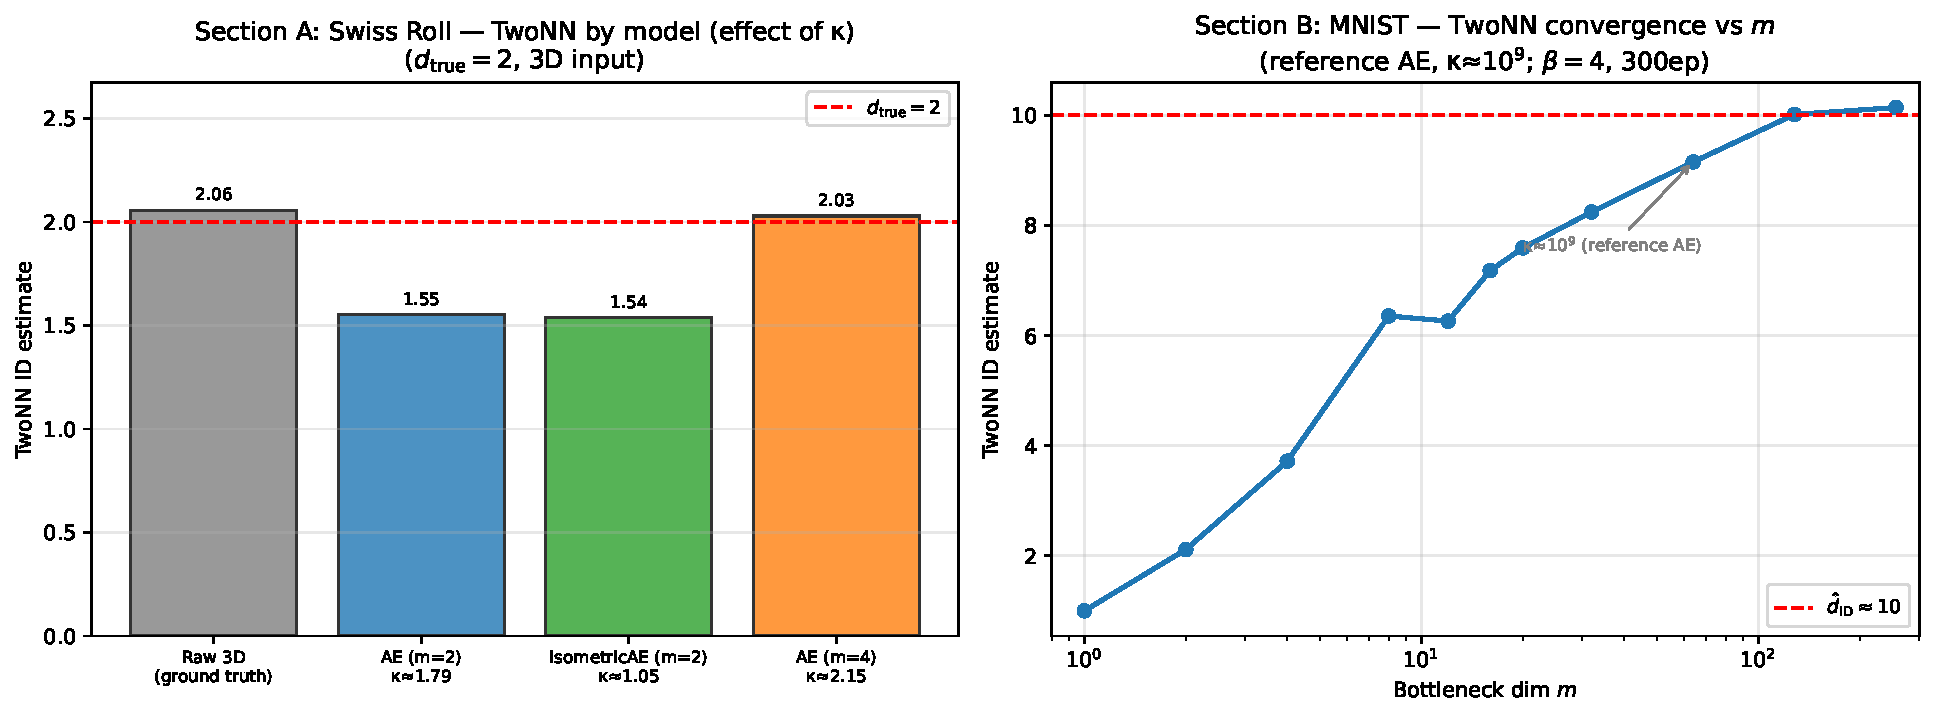
\includegraphics[width=0.95\linewidth]{results/figures/EP_twonn_stability.pdf}
  \caption{Exp-Stab/Exp-Geom: (Left) TwoNN ID on Swiss Roll --- AE and IsometricAE both underestimate at $m=d_\mathrm{true}$; TwoNN recovers at $m=4>d_\mathrm{true}$. (Right) MNIST AE $m$-sweep: TwoNN stabilizes at $m \geq 48$ despite $\kap$ jumping to $37.0$ at $m=128$. Detailed tables in Appendix~\ref{app:twonn_detail}.}
  \label{fig:ep}
\end{figure}}{}
\subsection{MNIST: Reading Off the Effective Representation Dimensionality (Main Experiments, RQ1 and RQ2)}\label{sec:exp_mnist}

We validate the application of the proposed framework to real data using the MNIST dataset (main experiments).
MNIST provides a realistic evaluation environment for the framework in the sense that it is
``real data for which $\dtrue$ is unknown but $\hat{d}_\mathrm{ID}$ can be estimated.''

\subsubsection{Intrinsic-Dimension Estimation with an AE (Experiment Exp-Mnist-Base-AE)}

Table~\ref{tab:e4_ae} shows the results for the MNIST AE (300 epochs).

\begin{table}[H]
\centering
\caption{Exp-Mnist-Base: MNIST AE results (300 epochs, $n_\mathrm{train}=20{,}000$; \textbf{single seed 42}).}
\label{tab:e4_ae}
\small
\begin{tabular}{rcccc}
\toprule
$m$ & MSE & TwoNN ID & MLE ID & CKA \\
\midrule
1   & 0.0437 & 1.02  & 1.15  & 0.102 \\
4   & 0.0292 & 3.86  & 4.29  & 0.575 \\
8   & 0.0191 & 6.08  & 6.70  & 0.725 \\
16  & 0.0121 & 7.96  & 8.61  & 0.812 \\
32  & 0.0087 & 8.84  & 9.89  & 0.875 \\
64  & 0.0062 & 9.54  & 11.26 & 0.908 \\
128 & 0.0061 & 9.84  & 11.45 & 0.921 \\
256 & 0.0057 & \textbf{10.02} & \textbf{11.85} & 0.953 \\
\bottomrule
\end{tabular}
\end{table}

For $m \geq 64$, the TwoNN ID (9.54--10.02) and the MLE ID (11.26--11.85) converge,
indicating that the effective intrinsic dimension of MNIST lies roughly in the range
$\hat{d}_\mathrm{ID} \approx 10$--12.

\textbf{Comparison with linear PCA}:
Applying PCA to MNIST ($n = 20{,}000$) requires 43 dimensions to reach 80\% cumulative
explained variance and 86 dimensions to reach 90\%.
These values are 4--8 times larger than the AE-based estimate (TwoNN $\approx 10$),
demonstrating the nonlinear manifold structure of MNIST (see Figure~\ref{fig:e4_dualaxis}).

\subsubsection{VAE AU Dynamics and $\mknee$ (Experiment Exp-Mnist-Base-VAE)}

Table~\ref{tab:e4_vae} and Figure~\ref{fig:e4_dualaxis} show the AU pattern of the MNIST VAE
($\beta = 4$, 300 epochs).

\begin{table}[H]
\centering
\caption{Exp-Mnist-Base: MNIST VAE ($\beta=4$) results (300 epochs; \textbf{single seed 42}). AU increase rate slows at $m=12$ ($\mknee=12$; preliminary, not reproduced in multi-seed runs).}
\label{tab:e4_vae}
\small
\begin{tabular}{rcccc}
\toprule
$m$ & MSE & AU & TwoNN ID & Behavior of $\rho(m)$ \\
\midrule
1   & 0.0464 & 1  & 1.00 & --- \\
4   & 0.0275 & 4  & 3.72 & normal growth \\
8   & 0.0186 & 8  & 6.36 & normal growth \\
\textbf{12} & 0.0184 & \textbf{8}  & 6.26 & \textbf{sharp drop} $\leftarrow \mknee = 12$ \\
16  & 0.0148 & 11 & 7.18 & low \\
20  & 0.0134 & 13 & 7.59 & low \\
32  & 0.0121 & 15 & 8.25 & low \\
64  & 0.0103 & 29 & 9.16 & gradual \\
128 & 0.0085 & 26 & 10.02 & gradual \\
256 & 0.0072 & 36 & 10.14 & gradual \\
\bottomrule
\end{tabular}
\end{table}

At $m = 12$, AU $= 8$ (the same value as at the preceding $m = 8$), and the normalized
increase rate $\rho(m)$ drops sharply ($\rho(12) \approx 0$).
This triggers the threshold $\tau_{\mathrm{knee}} = 0.25$, and $\mknee = 12$ is observed.

\textbf{Caveat}: this $\mknee = 12$ is a preliminary observation obtained with a single
seed (seed 42) and a specific extended grid ($m \in \{1,4,8,\ldots,256\}$), and it does
not reproduce in the multi-seed experiments (Section~\ref{sec:exp_multiseed})
(the main stabilized result of this paper is Exp-Mnist-Dense-300;
Section~\ref{sec:exp_el}).

\IfFileExists{results/figures/E4_mnist_dualaxis.pdf}{%
\begin{figure}[H]
\centering
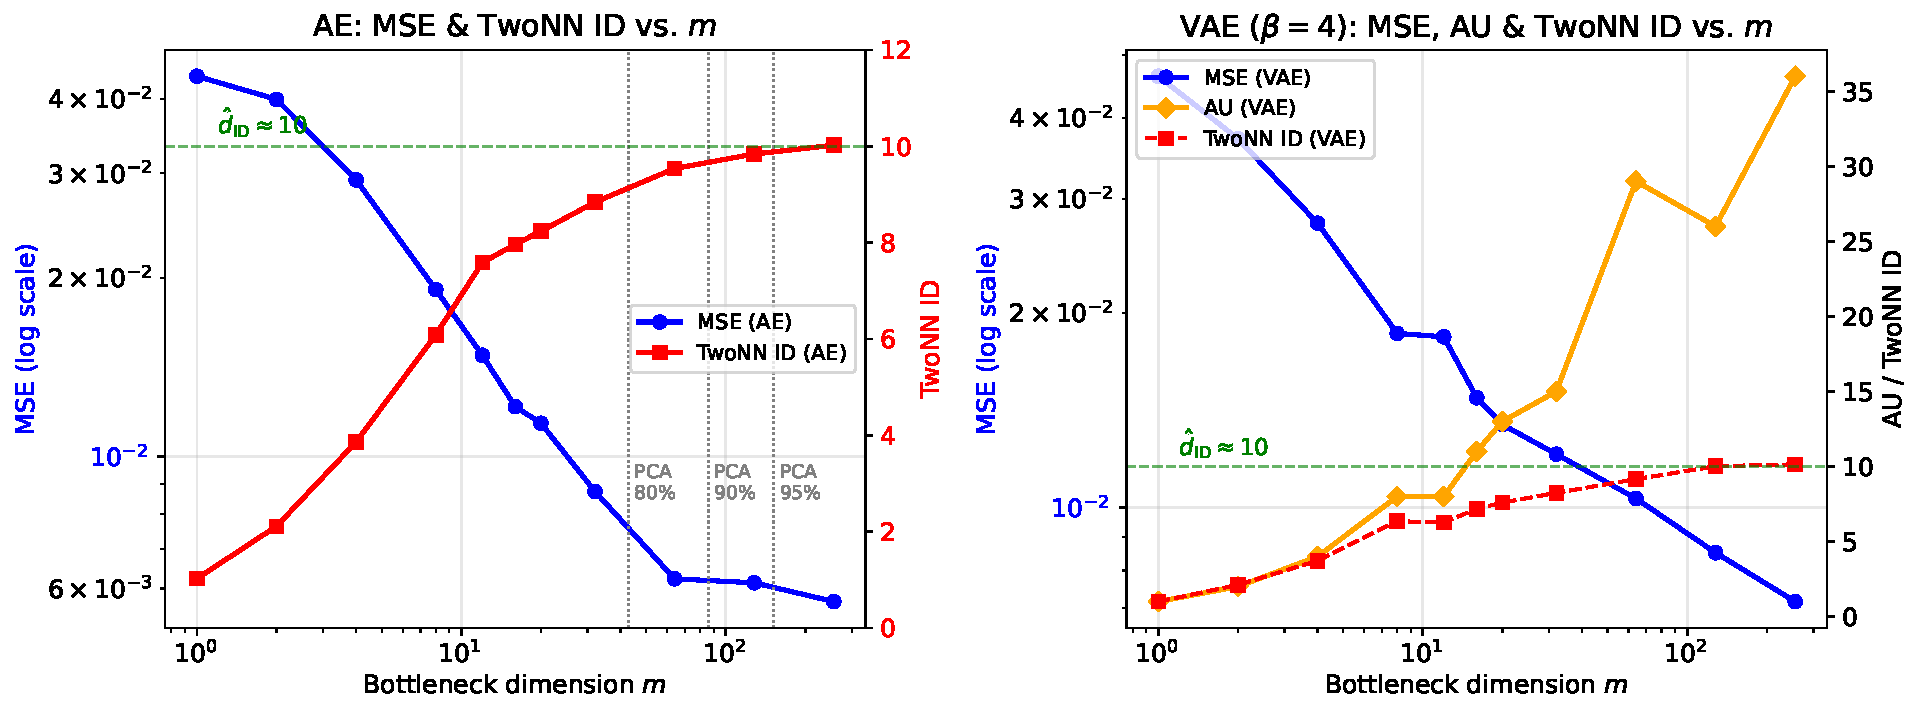
\includegraphics[width=0.95\linewidth]{results/figures/E4_mnist_dualaxis.pdf}
\caption{Exp-Mnist-Base: $m$-dependence of each indicator for MNIST (300 epochs). \textbf{Left (AE)}: MSE (log scale, left axis) and TwoNN ID (right axis). Vertical dotted lines correspond to PCA cumulative variance 80\% (43 dims), 90\% (86 dims), 95\% (152 dims); the difference from the nonlinear AE estimate (TwoNN $\approx 10$) is clear. \textbf{Right (VAE, $\beta=4$)}: MSE (log scale, left axis), AU (right axis), TwoNN ID (right axis, dashed). At $m = 12$ ($\mknee$), the AU increase rate drops sharply (arrow), indicating a heuristic slowdown point; the main stabilized result is $\mknee=10.3\pm0.9$ from Exp-Mnist-Dense-300 (Section~\ref{sec:exp_el}).}
\label{fig:e4_dualaxis}
\end{figure}}{}%

\subsubsection{Comparison with Existing Indicators}\label{sec:exp_comparison}

We compare the proposed indicator $\mknee$ with other representative indicators for choosing
the bottleneck dimension (Table~\ref{tab:method_comparison}).

\begin{table}[H]
\begin{adjustwidth}{-\extralength}{0cm}
\centering
\caption{Comparison of bottleneck dimension estimates on MNIST. $\mknee$ entries distinguish sparse-grid and dense-grid conditions.}
\label{tab:method_comparison}
\small
\begin{tabular}{p{4.0cm}cc p{4.5cm}}
\toprule
Method & Estimate & Source & Characteristics / Limitations \\
\midrule
PCA (80\% var.) & 43 & Exp-Mnist-Base-AE & Linear; overestimates nonlinear ID \\
PCA (90\% var.) & 86 & Exp-Mnist-Base-AE & Linear; larger overestimate \\
MSE elbow (AE) & $\approx16$--$20$ & Exp-Mnist-Base-AE & Intuitive; depends on smoothing \\
TwoNN ID (ref.\ AE) & $\approx10$--$12$ & Exp-Mnist-Base-AE & Nonlinear; subject to isometry bias \\
\midrule
$\mknee$ sparse-grid (3 seeds) & $43\pm15$ & Exp-Mnist-Multi-300 & Exploratory; unreliable at sparse grid \\
$\mknee$ \textbf{dense-grid (3 seeds)} & $\boldsymbol{10.3\pm0.9}$ & \textbf{Exp-Mnist-Dense-300} & \textbf{TwoNN-guided local refinement; requires dense grid + multi-seed} \\
\midrule
\multicolumn{4}{p{13.5cm}}{\footnotesize Dense-grid: $m\in\{8,9,\ldots,16,18,\ldots,64\}$ with independent initialization per $(m,\mathrm{seed})$; the dense region was placed around the TwoNN estimate ($\approx10$), so the agreement is a TwoNN-guided refinement, not an independent validation. Sparse-grid $\mknee=43\pm15$ is unreliable as a diagnostic reference.} \\
\bottomrule
\end{tabular}
\end{adjustwidth}
\end{table}

PCA, being linear, cannot capture the nonlinear manifold structure and requires more than
four times as many dimensions as the AE-based estimate, while the MSE elbow tends to be
ambiguous on smooth MSE curves.
$\mknee$ is complementary to these indicators in that it directly observes the KL dynamics,
but it depends on $\tau$, $\beta$, and the $m$-grid, and its use presupposes the
multi-indicator approach.

\subsubsection{Multi-Seed Validation (Experiments Exp-Mnist-Multi-150 and Exp-Mnist-Multi-300)}\label{sec:exp_multiseed}
\label{sec:exp_multiseed2}

To assess the statistical reliability of $\mknee$ and the influence of the degree of
convergence, we trained the MNIST VAE ($\beta = 4$, $m \in \{4,8,12,16,20,32,64\}$)
with three random seeds (42, 123, 777) under two conditions: 150 epochs
(Exp-Mnist-Multi-150) and 300 epochs (Exp-Mnist-Multi-300).
Table~\ref{tab:e4_300ep_multiseed} shows the 300-epoch results
(the 150-epoch $\mknee$ values are summarized in Table~\ref{tab:el_mknee};
the AU and TwoNN ID trends are identical to the 300-epoch condition, with the
TwoNN ID at $m=64$ being $9.94 \pm 0.08$).

\begin{table}[H]
\centering
\caption{Exp-Mnist-Multi-300: Mean$\pm$std of AU and TwoNN ID for 3 seeds at 300 epochs ($\beta=4$). AU and TwoNN ID are highly consistent, but $\mknee$ still varies.}
\label{tab:e4_300ep_multiseed}
\small
\begin{tabular}{rccl}
\toprule
$m$ & AU (mean$\pm$std) & TwoNN ID (mean$\pm$std) & Note \\
\midrule
 4 & $4.0 \pm 0.0$ & $3.98 \pm 0.14$ & all dims active \\
 8 & $8.0 \pm 0.0$ & $6.67 \pm 0.15$ & \\
12 & $10.0 \pm 0.0$ & $7.41 \pm 0.06$ & \\
16 & $11.7 \pm 0.5$ & $7.95 \pm 0.21$ & AU still increasing \\
20 & $13.3 \pm 0.5$ & $8.37 \pm 0.14$ & \\
32 & $15.7 \pm 0.5$ & $9.07 \pm 0.10$ & \\
64 & $22.3 \pm 0.5$ & $10.03 \pm 0.12$ & converges to $\hat{d}_\mathrm{ID} \approx 10$ \\
\midrule
\multicolumn{4}{l}{$\mknee$ ($\tau=0.25$): seed 42 $=$ 64, seed 123 $=$ 32, seed 777 $=$ 32} \\
\multicolumn{4}{l}{Mean $\mknee = 43 \pm 15$ (300 epochs)} \\
\bottomrule
\end{tabular}
\end{table}

\IfFileExists{results/figures/E4_300ep_multiseed.pdf}{%
\begin{figure}[H]
  \centering
  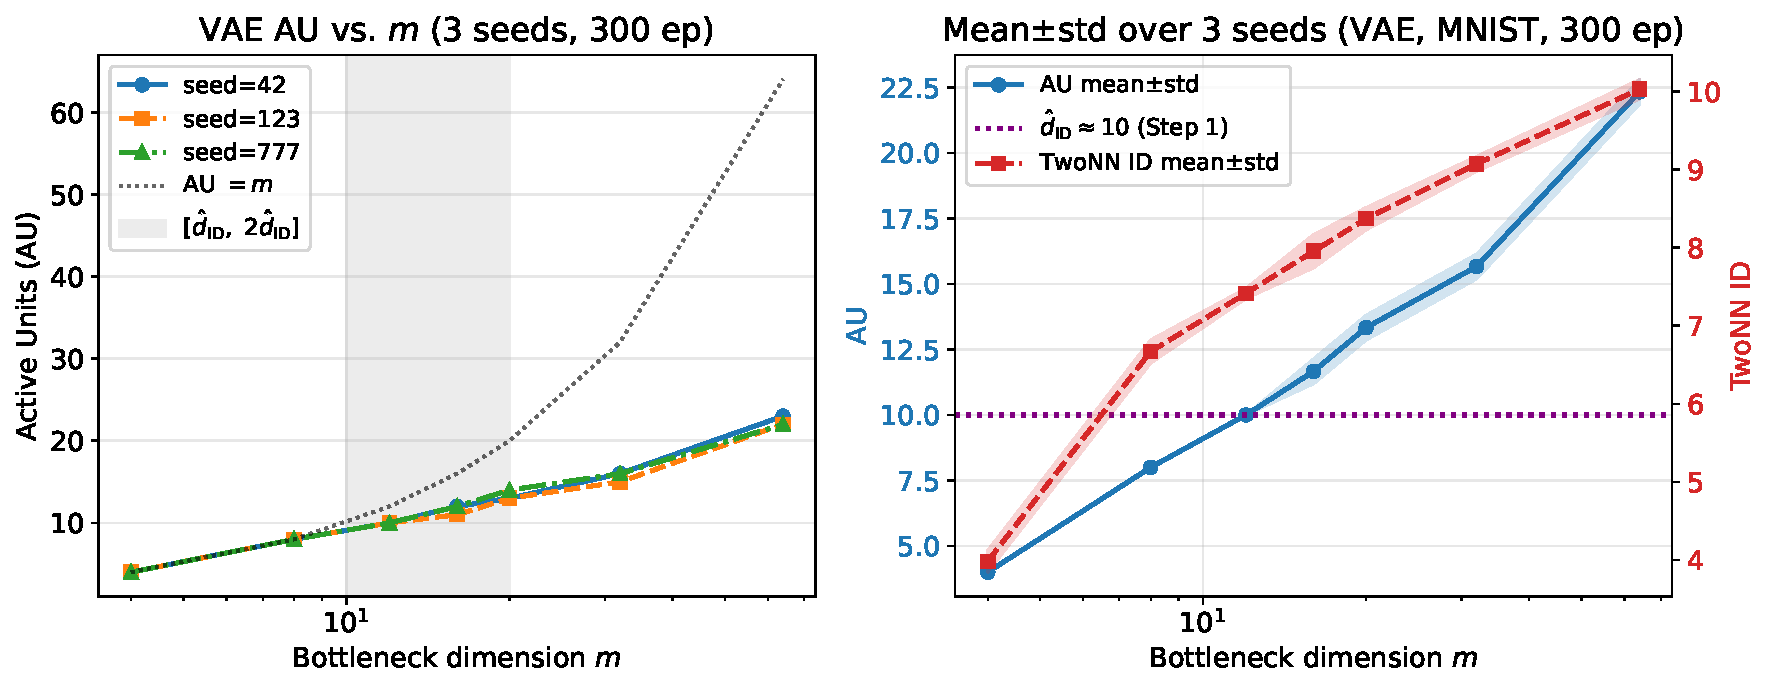
\includegraphics[width=0.9\linewidth]{results/figures/E4_300ep_multiseed.pdf}
  \caption{Exp-Mnist-Multi: AU patterns of MNIST VAE (3 seeds, 300 epochs). Left: AU vs $m$ per seed (dotted lines: $\mknee$); Right: mean$\pm$std band. AU and TwoNN ID bands are very narrow, but $\mknee$ varies between 32 and 64 across seeds.}
  \label{fig:e4_300ep_multiseed}
\end{figure}}{}

\textbf{Key findings}:
The AU values (Table~\ref{tab:e4_300ep_multiseed}) are highly consistent across the three
seeds under both epoch conditions ($\sigma \leq 0.5$), and the TwoNN ID is likewise stable
at $10.03 \pm 0.12$ for $m = 64$ (300 epochs).
In contrast, $\mknee$ ($\tau=0.25$) varied over the range 32--64 in both conditions:
$53 \pm 15$ at 150 epochs (per-seed 64, 32, 64) and $43 \pm 15$ even under full
300-epoch convergence (per-seed 64, 32, 32).
This occurs because the normalized increase rate $\rho(m)$ fluctuates subtly around the
threshold $\tau = 0.25$ over several values of $m$, and extending training does not resolve
it---\textbf{the dominant cause of the $\mknee$ instability is not insufficient convergence
but the dependence on the $m$-grid and the random seed}.
The $\mknee = 12$ observed in the extended Exp-Mnist-Base experiment (single seed 42) also
fails to reproduce under these conditions and remains a preliminary observation dependent
on the grid design and initialization trajectory (stabilization conditions in
Section~\ref{sec:exp_el}).

\subsubsection{Linear Theory--Experiment Bridge (Experiment Exp-Mnist-PCA; Details in Appendix~\ref{app:twonn_detail})}\label{sec:exp_em}

Contrasting the MNIST PCA spectrum ($\lambda_1=5.22, \ldots, \lambda_{10}=1.23$) with
Theorem~\ref{thm:linear_vae}, we obtain $d^* \approx 10$ for
$\tau^2_\mathrm{eff} \approx 0.30$ (back-calculated), qualitatively consistent with the
observed TwoNN ID.
Whereas the linear setting produces a sharp saturation transition, in nonlinear VAEs gradient
competition yields a smooth, gradually increasing curve, which theoretically corroborates the
sparse-grid instability of $\mknee$ (detailed PCA spectrum tables and theory--experiment
comparison tables are given in Appendix~\ref{app:twonn_detail}).
For Conv-VAEs, the powerful reconstruction capability of the nonlinear decoder makes
$\tau^2_\mathrm{eff}$ even smaller, so the $m$ required for AU saturation increases
substantially relative to the FC-VAE (Section~\ref{sec:disc_convvae}).

\subsubsection{TwoNN-Guided Local Refinement with a Dense Grid (Experiment Exp-Mnist-Dense)}\label{sec:exp_el}

To identify which factors cause the instability of $\mknee$, we designed an
experiment that isolates three factors: grid density, epochs, and seed.
Exp-Mnist-Base and Exp-Mnist-Multi already separate the epoch factor (150 ep vs.\ 300 ep) and
the seed factor (3 seeds).
The present experiment, Exp-Mnist-Dense, further isolates the grid-density factor: we trained
with $m \in \{8,9,10,11,12,13,14,15,16,18,20,24,28,32,40,48,64\}$
(17 points, adjacent spacing 1--16; step 1 over $m=8$--$16$ near the estimated ID) for 300 epochs and 3 seeds.
\textbf{Explicit positioning}: the dense region ($m = 8$--16) was placed around the Stage-1
TwoNN estimate ($\hat{d}_\mathrm{ID} \approx 10$), so the choice of the candidate region
itself depends on the TwoNN estimate of the same framework.
Consequently, the agreement between $\mknee$ and the TwoNN ID reported below demonstrates
the success of a \textbf{TwoNN-guided local refinement}, not a mutual validation
independent of TwoNN
(securing independence---via a pre-registered dense grid over a broader range, or nested
validation in which the search region is estimated and $\mknee$ is evaluated on disjoint
seeds or data subsets---is left as future work).

\begin{table}[H]
\begin{adjustwidth}{-\extralength}{0cm}
\centering
\caption{Exp-Mnist-Dense: Comparison of $\mknee$ between dense and sparse grids ($\tau=0.25$, MNIST FC-VAE, $\beta=4$). Consistent with the grid-sensitivity bound of Proposition \ref{thm:mknee_instab}.}
\label{tab:el_mknee}
\small
\begin{tabular}{lccccc}
\toprule
Condition & Max.\ grid interval & seed=42 & seed=123 & seed=777 & Mean$\pm$std \\
\midrule
Sparse grid, 150ep (Exp-Mnist-Multi-150) & 32 & 64 & 32 & 64 & $53 \pm 15$ \\
Sparse grid, 300ep (Exp-Mnist-Multi-300) & 32 & 64 & 32 & 32 & $43 \pm 15$ \\
Dense, 300ep (Exp-Mnist-Dense-300) & 16 (step 1, 8--16) & 11 & 9 & 11 & $10.3 \pm 0.9$ \\
\bottomrule
\end{tabular}
\end{adjustwidth}
\end{table}

\begin{table}[H]
\begin{adjustwidth}{-\extralength}{0cm}
\centering
\caption{Exp-Mnist-Dense: Per-seed AU$(m)$ curves for the full dense grid (300ep, all 3 seeds). The AU curves fluctuate non-monotonically in the transition region ($m=11$--$16$).}
\label{tab:el_au}
\small
\begin{tabular}{l*{17}{c}}
\toprule
$m$ & 8 & 9 & 10 & 11 & 12 & 13 & 14 & 15 & 16 & 18 & 20 & 24 & 28 & 32 & 40 & 48 & 64 \\
\midrule
AU (seed 42)  & 8 & 9 & 10 & 10 & 10 & 10 & 12 & 11 & 14 & 13 & 15 & 14 & 15 & 15 & 18 & 19 & 21 \\
AU (seed 123) & 8 & 8 & 10 & 9  & 11 & 10 & 11 & 13 & 12 & 14 & 13 & 15 & 14 & 17 & 19 & 19 & 21 \\
AU (seed 777) & 8 & 9 & 10 & 10 & 11 & 10 & 11 & 11 & 12 & 12 & 13 & 15 & 16 & 18 & 18 & 20 & 21 \\
\bottomrule
\end{tabular}
\end{adjustwidth}
\end{table}

\IfFileExists{results/figures/EL_dense_grid_mknee.pdf}{%
\begin{figure}[H]
  \centering
  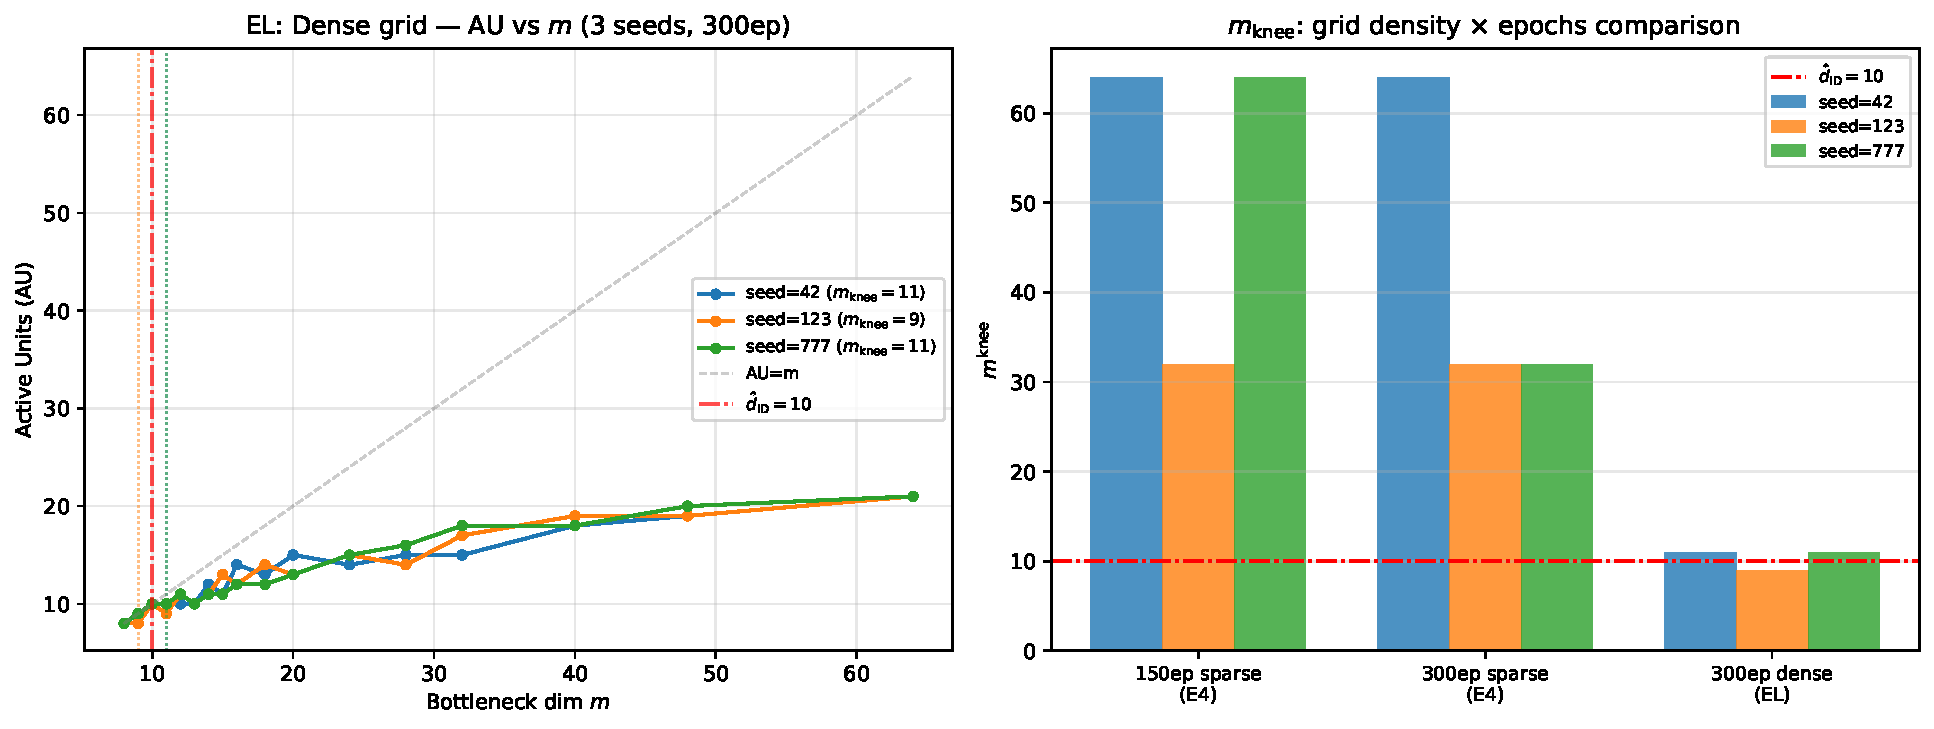
\includegraphics[width=0.95\linewidth]{results/figures/EL_dense_grid_mknee.pdf}
  \caption{Exp-Mnist-Dense: (Left) Dense-grid AU vs $m$ (3 seeds). (Right) Comparison by grid density $\times$ epochs. $\mknee$ variation in the dense grid can be assessed by the upper bound of Proposition~\ref{thm:mknee_instab} (maximum grid interval).}
  \label{fig:el}
\end{figure}}{}

\textbf{Isolation of the three factors}:
The three-row comparison in Table~\ref{tab:el_mknee} quantitatively isolates the
epoch factor (150 ep $\to$ 300 ep: $53\pm15 \to 43\pm15$; a slight stabilization,
not the main cause), the seed factor ($\sigma = 15$ under identical conditions; a
secondary factor), and the grid-density factor (dense grid:
$\mknee = 10.3 \pm 0.9$, per-seed 11, 9, 11).
The effect of grid density is qualitatively consistent with the implication of
Proposition~\ref{thm:mknee_instab} (grid design matters in the idealized model),
but since empirical AU curves exhibit non-monotone fluctuations
(e.g., AU$=10 \to 10 \to 10 \to 12 \to 11$ in Table~\ref{tab:el_au}), it is more
accurate to state the result as ``densifying the grid greatly reduced the
variance of the empirical $\mknee$'' rather than to claim that the deviation
``stayed within the upper bound.''
We note again that the agreement with the TwoNN ID ($\approx 10$) is a
consequence of the TwoNN-guided refinement, since the dense region was placed
around the TwoNN estimate.

\noindent
\textbf{Comparison of the $\tau$-method and the second-difference method}:
Besides the first-difference ratio method adopted in this paper ($\tau = 0.25$), $\mknee$ can
be detected by the \textbf{second-difference method}, which locates the point of maximum
curvature of the AU$(m)$ curve (Appendix~\ref{app:tau_knee}).
Table~\ref{tab:el_knee_compare} shows the comparison on the Exp-Mnist-Dense dense-grid data.

\begin{table}[H]
\centering
\caption{Exp-Mnist-Dense: Comparison of $\tau$-method ($\tau=0.25$) and second-difference method (d2) for $\mknee$ detection (dense grid, 300ep, 3 seeds).}
\label{tab:el_knee_compare}
\small
\begin{tabular}{lcccc}
\toprule
Method & seed=42 & seed=123 & seed=777 & Mean$\pm$std \\
\midrule
$\tau$-method ($\tau=0.25$) & 11 & 9  & 11 & $10.3 \pm 0.9$ \\
Second-difference method (d2) & 15 & 28 & 12 & $18.3 \pm 6.8$ \\
\midrule
\multicolumn{5}{l}{Reference: $\hat{d}_\mathrm{ID} \approx 10$ (TwoNN, $m=64$, 3-seed mean)} \\
\bottomrule
\end{tabular}
\end{table}

The $\tau$-method yields a mean of $10.3 \pm 0.9$, consistent with
$\hat{d}_\mathrm{ID} \approx 10$, with small seed-to-seed variation.
In contrast, the d2 method is sensitive to the discrete noise of AU$(m)$; for seed=123 it
deviated strongly to $\mknee = 28$ (in the transition region the AU curve fluctuates as
$8 \to 10 \to 9 \to 11 \to 10 \to 11 \to 13$, which perturbs the location of the maximum
second difference).
Therefore, \textbf{the $\tau$-method is the more stable choice for detecting $\mknee$ under
dense-grid conditions}, and we position the d2 method as an auxiliary tool for locating
global ``elbow'' candidates (see Appendix~\ref{app:tau_knee}).

Finally, the fact that the MNIST VAE reaches $\AUsat = 36$ ($m=256$), substantially exceeding
$\hat{d}_\mathrm{ID} \approx 10$--12 (the Manifold Entanglement hypothesis), and the
two-phase pattern of the training dynamics (Exp-Mnist-Dyn) are both single-seed, preliminary
observations; multi-seed validation of these is left for future work
(see Section~\ref{sec:disc_incidental}).
\subsection{Application to Fashion-MNIST (Experiment Exp-Fashion, Exploratory Supplementary Evidence)}\label{sec:exp_fashion}

Fashion-MNIST (10 clothing classes, $28\times28$; 100 epochs, \textbf{single seed 42})
lacks multi-seed verification and is therefore positioned as
\textbf{exploratory supplementary evidence rather than an external validation};
the detailed result table and figure are moved to Appendix~\ref{app:fashion}
(Table~\ref{tab:ef}, Figure~\ref{fig:ef}).
In brief: for the AE, TwoNN ID converges to $\approx 9.4$ at $m \geq 32$,
suggesting $\hat{d}_\mathrm{ID} \approx 9$--$10$;
for the VAE ($\beta = 4$), $\mknee = 12$ ($\tau_{\mathrm{knee}} = 0.25$) was
observed, but this is an exploratory single-seed observation and we do not claim
the same level of reproducibility as the MNIST three-seed experiments.
Multi-seed replication on Fashion-MNIST is left as future work
(note that Exp-Real-Geom, which includes Fashion-MNIST, provides multi-seed
real-data evidence; Section~\ref{sec:exp_real_geom}).

\subsection{Extension to Convolutional Architectures (Experiment Exp-Conv-AE)}\label{sec:exp_conv}

To address concerns about generalizability when the study is limited to fully connected architectures,
we applied convolutional AE/VAE (Conv-AE/VAE) to MNIST (Experiment Exp-Conv-AE;
100 epochs, $m \in \{4, 8, 12, 16, 20, 32, 64\}$, \textbf{single seed 42};
architecture details and the result table are given in Appendix~\ref{app:fashion},
Table~\ref{tab:eg}).

The \textbf{Conv-AE TwoNN ID} converges to $11.29$ at $m = 64$, consistent with the FC-AE
estimate ($\approx 10$, within $\approx 10\%$)---TwoNN estimates are consistent across
architectures (an empirical observation under the conditions of this study).
The \textbf{Conv-VAE}, in contrast, shows AU $= m$ (no saturation) for $m \leq 32$:
at 100 epochs the KL-driven dimension suppression is not yet functioning, and reliable
detection of $\mknee$ requires a larger number of epochs.

\subsubsection{Delayed AU Saturation in Conv-VAEs: Fixed-$\beta$ vs.\ KL-Annealing Comparison (Experiments Exp-Conv-Fix and Exp-Conv-Ann)}
\label{sec:exp_conv_300ep}

Following the insufficient convergence in Exp-Conv-AE, we verified with 300 epochs and 3 seeds (Exp-Conv-Fix)
and with KL cyclic annealing (Exp-Conv-Ann)
(Table~\ref{tab:eh_conv_vae}).

\begin{table}[H]
\begin{adjustwidth}{-\extralength}{0cm}
\centering
\caption{Exp-Conv-Fix and Exp-Conv-Ann: Comparison of AU for MNIST Conv-VAE (300ep, mean$\pm$std over 3 seeds). FC-VAE (Exp-Mnist-Multi-300) slows down by $m=32$ (AU$=15.7$), while Conv-VAE shows AU$=m$ (no saturation) under both fixed-$\beta$ and annealing at $m \leq 32$.}
\label{tab:eh_conv_vae}
\small
\begin{tabular}{r ccc cc}
\toprule
 & \multicolumn{2}{c}{Conv-VAE fixed-$\beta$ (Exp-Conv-Fix)} & \multicolumn{1}{c}{Conv-VAE annealing (Exp-Conv-Ann)} & \multicolumn{2}{c}{FC-VAE (Exp-Mnist-Multi-300)} \\
$m$ & AU & TwoNN ID & AU & AU & TwoNN ID \\
\midrule
 4 & $4.0\pm0.0$ & $3.97\pm0.08$ & $4.0\pm0.0$ & $4.0$ & $3.98$ \\
12 & $12.0\pm0.0$ & $8.14\pm0.09$ & $12.0\pm0.0$ & $10.0$ & $7.41$ \\
32 & $32.0\pm0.0$ & $11.43\pm0.08$ & $32.0\pm0.0$ & $15.7$ & $9.07$ \\
64 & $54.3\pm0.5$ & $13.10\pm0.05$ & $64.0\pm0.0$ & $22.3$ & $10.03$ \\
\midrule
\multicolumn{6}{l}{$\mknee$: Conv-VAE (both conditions) all seeds $=64$ (grid upper bound); FC-VAE $=43\pm15$ (32--64)} \\
\bottomrule
\end{tabular}
\end{adjustwidth}
\end{table}

The Conv-VAE exhibits AU$=m$ (no saturation) for $m \leq 32$ under both fixed $\beta=4$ and cyclic annealing,
making the divergence from the FC-VAE clear (theoretical discussion in \S\ref{sec:disc_convvae}).
AU$\approx m$ is a signal that ``KL regularization is not yet functioning,'' and in this state the TwoNN ID
is also inflated (Conv-VAE $m=64$: $13.10$ vs.\ FC-VAE: $10.03$).
\textbf{On the grid $m \leq 64$, AU saturation cannot be observed}, and an extension of the $m$ range is required.

%% ===================================================================
\subsection{Conv-VAE Extended $m$-Grid Experiments (Experiments Exp-Conv-M256 and Exp-Conv-M512)}\label{sec:exp_en}

Since no AU saturation was observed for $m \leq 64$ in Exp-Conv-Fix and Exp-Conv-Ann (\S\ref{sec:exp_conv_300ep}),
we extended the $m$ grid to 256 (Experiment Exp-Conv-M256) and 512 (Experiment Exp-Conv-M512).
Under the reduced-$\tau^2_\mathrm{eff}$ hypothesis discussed in \S\ref{sec:disc_convvae},
the Conv-VAE's $d^*(\beta)$ is substantially larger than that of the FC-VAE ($\approx 10$),
so a slowdown of AU growth is predicted to appear in the region $m>64$.

\textbf{Experimental setup} (Exp-Conv-M256):
Using the same Conv-VAE architecture as Exp-Conv-Ann ($28\times28$ MNIST, 2-layer Conv encoder,
2-layer ConvTranspose decoder, KL cyclic annealing with $\beta_\mathrm{max}=4$, 3 cycles,
150 epochs, seeds$\in\{42,123,777\}$),
we tested $m \in \{4, 8, 16, 32, 64, 96, 128, 192, 256\}$ (9 points).

\begin{table}[H]
\centering
\caption{Exp-Conv-M256: Conv-VAE extended $m$ grid (KL annealing, 150 epochs, mean$\pm$std, 3 seeds). AU$=m$ for $m \leq 64$; AU$<m$ begins at $m \geq 96$. FC-VAE reference (Exp-Mnist-Multi-300, $m=64$): AU$=22.3\pm0.5$.}
\label{tab:en}
\small
\begin{tabular}{rccc}
\toprule
$m$ & AU (mean$\pm$std) & TwoNN ID (mean$\pm$std) & Note \\
\midrule
  4 & $4.0\pm0.0$   & $3.84\pm0.11$ & all dims active \\
  8 & $8.0\pm0.0$   & $6.64\pm0.11$ & \\
 16 & $16.0\pm0.0$  & $8.76\pm0.05$ & \\
 32 & $32.0\pm0.0$  & $10.46\pm0.13$ & \\
 64 & $64.0\pm0.0$  & $13.29\pm0.12$ & same as Exp-Conv-Ann (no saturation) \\
 96 & $\mathbf{90.7\pm1.2}$  & $14.30\pm0.22$ & \textbf{AU$<m$ onset} (FC-VAE $\hat{d}_\mathrm{ID} \approx 9\times$) \\
128 & $111.7\pm2.6$ & $14.69\pm0.13$ & \\
192 & $159.0\pm4.3$ & $15.89\pm0.27$ & \\
256 & $241.3\pm2.9$ & $16.58\pm0.16$ & \\
\midrule
\multicolumn{4}{l}{$\mknee$ ($\tau=0.25$): all seeds $=256$ (no knee within the tested range)} \\
\multicolumn{4}{l}{FC-VAE reference (Exp-Mnist-Multi-300, $m=64$): AU$=22.3\pm0.5$, TwoNN ID$=10.03\pm0.12$} \\
\bottomrule
\end{tabular}
\end{table}

\IfFileExists{results/figures/EN_conv_vae_extended_m.pdf}{%
\begin{figure}[H]
  \centering
  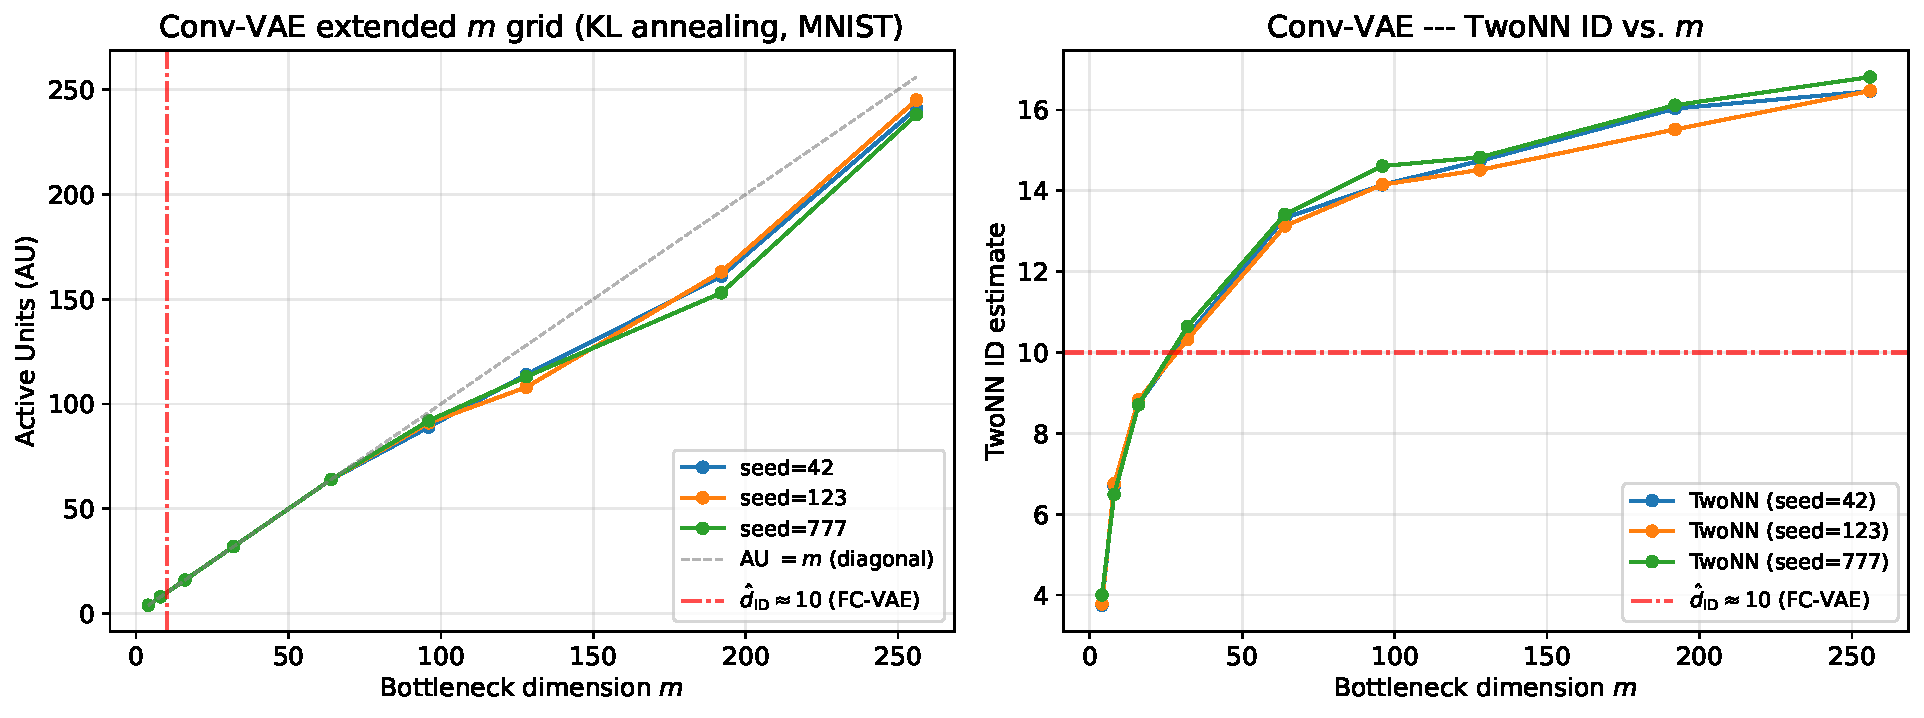
\includegraphics[width=0.95\linewidth]{results/figures/EN_conv_vae_extended_m.pdf}
  \caption{Exp-Conv-M256: Conv-VAE extended $m$ grid ($m\in[4,256]$, KL annealing, 3 seeds). AU vs $m$ (left) and TwoNN ID vs $m$ (right). Diagonal line (AU$=m$) and FC-VAE reference $\hat{d}_\mathrm{ID} \approx 10$ (red) are shown. AU$=m$ continues at $m \leq 64$ but deviates from the diagonal at $m \geq 96$, confirming qualitative water-filling behavior in Conv-VAE.}
  \label{fig:en}
\end{figure}}{}

\textbf{Main findings of Experiment Exp-Conv-M256}:
For $m \leq 64$, AU$=m$ holds across all 3 seeds (in stark contrast to the FC-VAE's
AU$=22.3$ at $m=64$); a saturation trend first appears at $m = 96$
(AU$=90.7\pm1.2 < m$), but even at $m=256$ the activation rate remains high (94.3\%) and
$\mknee$ stays pinned to the grid boundary (256) for all seeds.
This indicates that the Conv-VAE's $d^*(\beta)$ is substantially larger than the FC-VAE's
($\approx 10$), exceeding 256
(the correspondence with the $\tau^2_\mathrm{eff}$ theory is discussed in
\S\ref{sec:disc_convvae}).

\textbf{Extension beyond $m=256$ (Experiment Exp-Conv-M512, details in Appendix~\ref{app:convvae_natimg})}:
Even when extending to $m \in \{384, 512\}$, AU$\approx m$ (all dimensions active) is maintained across
all 3 seeds, and $\mknee$ remains pinned to the grid boundary at 512
(see Appendix~\ref{app:convvae_natimg}, Table~\ref{tab:en_ext}).
This shows that the $d^*(\beta)$ of the MNIST Conv-VAE exceeds $m=512$,
consistent with the $\tau^2_\mathrm{eff}$ theoretical prediction of \S\ref{sec:disc_convvae}.
In the next subsection, we show that AU saturation can be artificially induced by strengthening $\beta_{\max}$.

%% ===================================================================
\subsection{Artificially Inducing Conv-VAE AU Saturation with High $\beta$ (Experiment Exp-ConvV-HiBeta)}\label{sec:exp_hibeta}

As a verification of the $\tau^2_\mathrm{eff}$ hypothesis of \S\ref{sec:disc_convvae}
(a powerful decoder pushes AU saturation toward higher dimensions),
we increased $\beta_{\max}$ from $4$ to $\{10, 20\}$ and checked whether an AU saturation plateau
is induced in the MNIST Conv-VAE.

\textbf{Experimental setup}: Using the same architecture and KL cyclic annealing (3 cycles) as Exp-Conv-M256,
we trained with $\beta_{\max} \in \{10, 20\}$, $m \in \{16, 32, 64, 96, 128, 192, 256\}$,
seed=42, and 150 epochs (the $\beta_{\max}=4$, seed=42 results of Exp-Conv-M256 are reproduced for comparison).

\begin{table}[H]
\centering
\caption{Exp-ConvV-HiBeta: Comparison of MNIST Conv-VAE AU at $\beta_\mathrm{max} \in \{4, 10, 20\}$ (\textbf{single seed 42}, 150ep, KL cyclic annealing; exploratory). Higher $\beta_\mathrm{max}$ induces AU saturation at lower dimensions.}
\label{tab:hibeta}
\small
\begin{tabular}{r ccc}
\toprule
$m$ & $\beta_{\max}=4$ (Exp-Conv-M256) & $\beta_{\max}=10$ & $\beta_{\max}=20$ \\
\midrule
 16  & 16  (100\%)& 16 (100\%) & 16 (100\%) \\
 32  & 32  (100\%)& 32 (100\%) & 27 (84\%)  \\
 64  & 64  (100\%)& 54 (84\%)  & 42 (66\%)  \\
 96  & 89  (93\%) & 65 (68\%)  & 47 (49\%)  \\
128  & 114 (89\%) & 69 (54\%)  & 53 (41\%)  \\
192  & 161 (84\%) & 79 (41\%)  & 60 (31\%)  \\
256  & 241 (94\%) & 93 (36\%)  & 66 (26\%)  \\
\midrule
$\mknee$ ($\tau=0.25$) & 512 (grid boundary, unidentified) & $\approx 128$ & $\approx 96$ \\
\bottomrule
\end{tabular}
\end{table}

\textbf{Findings of Exp-ConvV-HiBeta} (Table~\ref{tab:hibeta}):
Whereas at $\beta_{\max}=4$ AU$=m$ (100\% active) persists for $m \leq 64$,
at $\beta_{\max}=10$ a clear AU saturation trend appears --- AU$=54$ (84\%) at $m=64$,
AU$=69$ (54\%) at $m=128$, and AU$=93$ (36\%) at $m=256$ ---
and $\mknee \approx 128$ ($\tau=0.25$) was identified.
Furthermore, at $\beta_{\max}=20$, saturation occurs at even lower dimensions ---
AU$=27$ (84\%) at $m=32$ and AU$=42$ (66\%) at $m=64$ --- and $\mknee \approx 96$ was observed.
This directly matches the prediction of the $\tau^2_\mathrm{eff}$ hypothesis of \S\ref{sec:disc_convvae}:
increasing $\beta$ shifts $d^*(\beta) = |\{j: \lambda_j > \beta\tau^2_\mathrm{eff}\}|$ to smaller values,
and AU saturation appears at lower dimensions.
\textbf{This result is consistent with the interpretation that the absence of observed AU saturation
in the MNIST Conv-VAE is not an ``applicability limit of the framework,'' but rather stems from the fact
that at the setting $\beta_{\max}=4$ the regularization was insufficient relative to the decoder capacity,
resulting in $d^*(\beta) \gg 256$.}
Applying the AU/$\mknee$ framework to Conv-VAEs requires an appropriate setting of $\beta$
matched to the data and architecture
(this experiment is a single-seed exploratory observation; multi-seed replication
is left as future work).

\IfFileExists{results/figures/Exp_ConvV_HiBeta.pdf}{%
\begin{figure}[H]
\centering
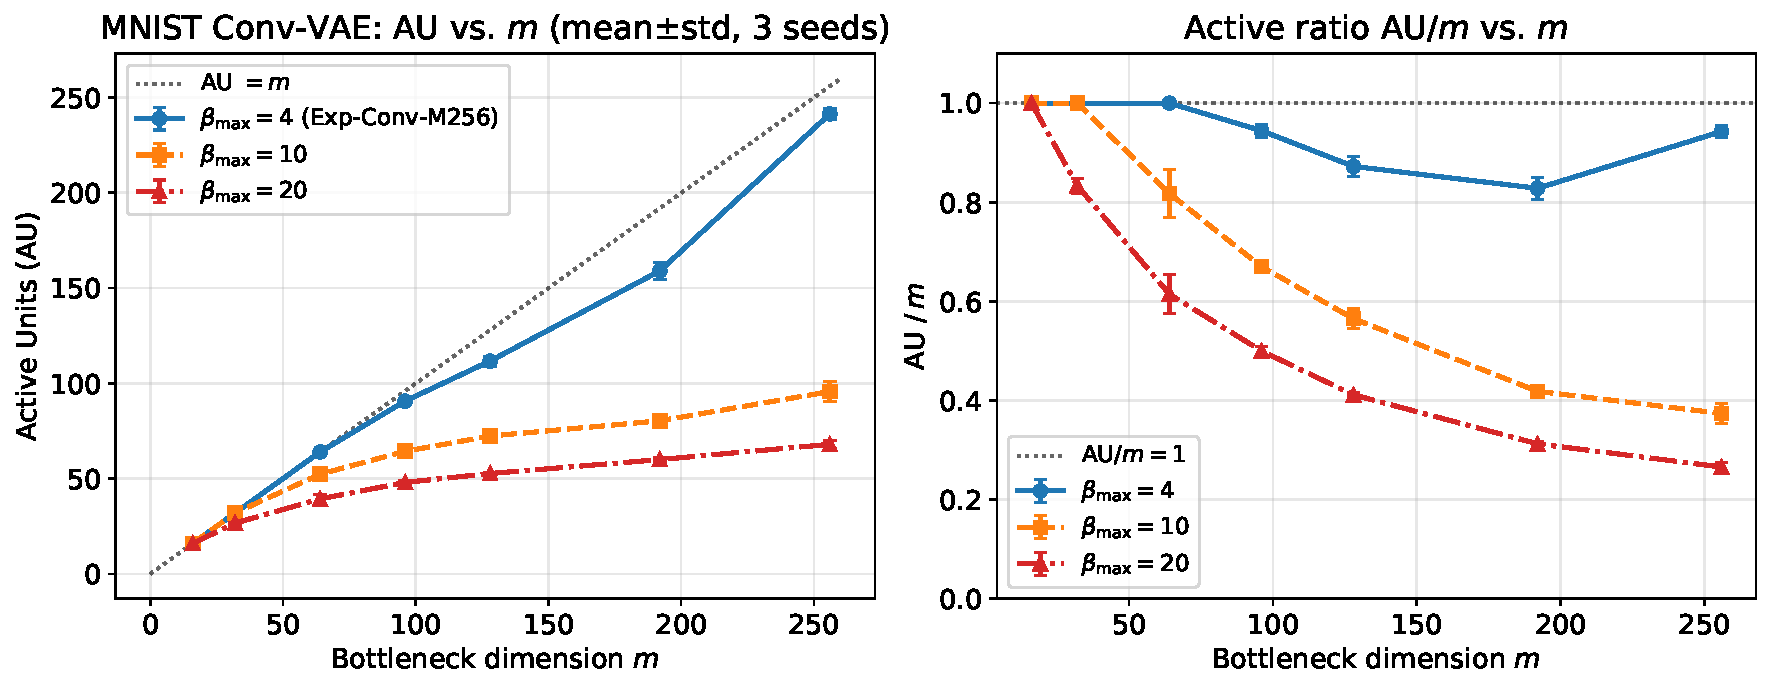
\includegraphics[width=0.9\linewidth]{results/figures/Exp_ConvV_HiBeta.pdf}
\caption{Exp-ConvV-HiBeta: Comparison of MNIST Conv-VAE AU vs $m$ (left) and activation rate AU/$m$ (right) for $\beta_{\max} \in \{4, 10, 20\}$. Increasing $\beta_{\max}$ shifts AU saturation to lower dimensions, demonstrating the $\beta$-dependence of $d^*(\beta)$.}
\label{fig:hibeta}
\end{figure}
}{}

%% ===================================================================
\subsection{Application to Natural Images: CIFAR-10 and SVHN (Experiments Exp-Nat-Cifar and Exp-Nat-SVHN)}\label{sec:exp_natural}

We applied the proposed framework to the more complex natural-image datasets
CIFAR-10~\cite{krizhevsky2009learning} and SVHN~\cite{netzer2011reading},
and compared the results with the intrinsic-dimension estimates reported by
Pope et al.~\cite{pope2021intrinsic}.

\textbf{Experimental setup} (Exp-Nat-Cifar: CIFAR-10; Exp-Nat-SVHN: SVHN):
a Conv-VAE (input $32 \times 32 \times 3$) with a three-layer Conv encoder
($3{\to}32{\to}64{\to}128$, $k=4$, stride 2) and a three-layer ConvTranspose
decoder was trained with $n_{\mathrm{train}} = 20{,}000$, 150 epochs,
KL cyclic annealing ($\beta_{\max}=4$, 3 cycles),
$m \in \{16, 32, 64, 128, 256\}$, and three seeds (42, 123, 777).

\begin{table}[H]
\begin{adjustwidth}{-\extralength}{0cm}
\centering
\caption{Exp-Nat-Cifar and Exp-Nat-SVHN: Conv-VAE results for CIFAR-10 (left) and SVHN (right) (mean$\pm$std, 3 seeds; KL cyclic annealing, 150 epochs, 3 cycles). At $m=64$, CIFAR-10 latent TwoNN ID converges to the raw-data value ($\approx25$), consistent with Pope et al.\ \cite{pope2021intrinsic} ($d_\mathrm{ID} \approx 26$).}
\label{tab:ei_ej}
\small
\begin{tabular}{r cc | cc}
\toprule
 & \multicolumn{2}{c|}{CIFAR-10 (Exp-Nat-Cifar)} & \multicolumn{2}{c}{SVHN (Exp-Nat-SVHN)} \\
$m$ & AU (mean$\pm$std) & TwoNN ID (mean$\pm$std) & AU (mean$\pm$std) & TwoNN ID (mean$\pm$std) \\
\midrule
 16  & $16.0\pm0.0$ & $13.12\pm0.12$ & $16.0\pm0.0$ & $11.30\pm0.12$ \\
 32  & $32.0\pm0.0$ & $19.26\pm0.23$ & $32.0\pm0.0$ & $15.08\pm0.08$ \\
 64  & $64.0\pm0.0$ & $\mathbf{25.21\pm0.41}$ & $64.0\pm0.0$ & $19.97\pm0.12$ \\
128  & $128.0\pm0.0$ & $28.83\pm0.41$ & $125.3\pm0.5$ & $24.60\pm0.36$ \\
256  & $256.0\pm0.0$ & $30.91\pm0.64$ & $206.7\pm1.2$ & $27.08\pm0.34$ \\
\midrule
\multicolumn{3}{l|}{Raw TwoNN=25.20, MLE=26.56 ($\approx$ Pope et al.\ estimate of 26)} & \multicolumn{2}{l}{Raw TwoNN=10.09, MLE=18.85} \\
\multicolumn{3}{l|}{$\mknee$ ($\tau=0.25$): all seeds=256 (no knee in range)} & \multicolumn{2}{l}{$\mknee$: all seeds=256 (no knee in range)} \\
\bottomrule
\end{tabular}
\end{adjustwidth}
\end{table}

\IfFileExists{results/figures/EI_cifar10_conv_vae.pdf}{%
\begin{figure}[H]
  \centering
  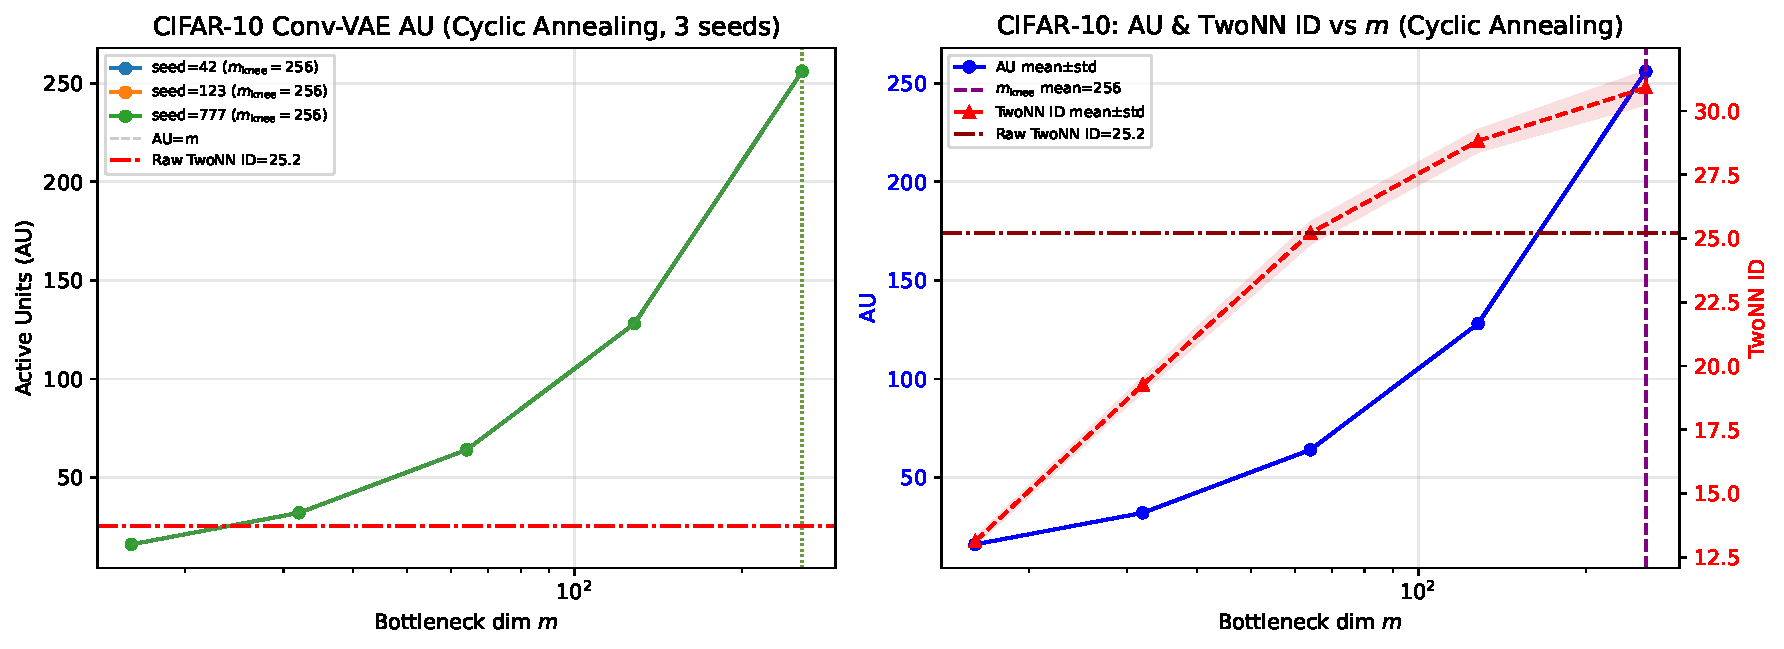
\includegraphics[width=0.95\linewidth]{results/figures/EI_cifar10_conv_vae.pdf}
  \caption{Exp-Nat-Cifar: $m$-dependence of AU and TwoNN ID for CIFAR-10 Conv-VAE (KL cyclic annealing, 3 seeds). TwoNN ID shows convergence consistent with Pope et al.\cite{pope2021intrinsic} ($d_\mathrm{ID} \approx 26$).}
  \label{fig:ei}
\end{figure}}{}

\IfFileExists{results/figures/EJ_svhn_conv_vae.pdf}{%
\begin{figure}[H]
  \centering
  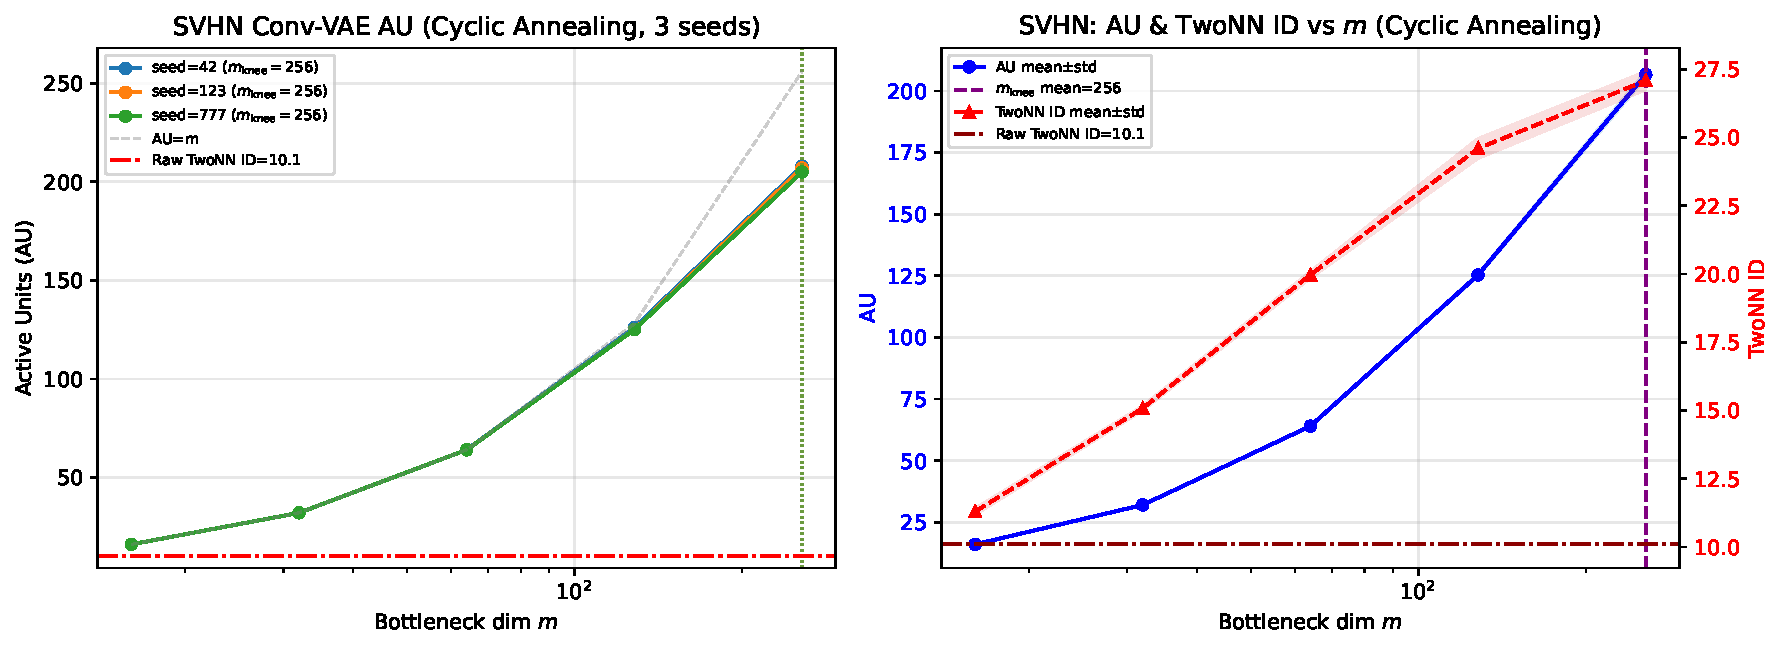
\includegraphics[width=0.95\linewidth]{results/figures/EJ_svhn_conv_vae.pdf}
  \caption{Exp-Nat-SVHN: $m$-dependence of AU and TwoNN ID for SVHN Conv-VAE (KL cyclic annealing, 3 seeds).}
  \label{fig:ej}
\end{figure}}{}

The primary aim of this experiment is limited to verifying whether the TwoNN ID
attains the same scale as the values reported by Pope et al.\ within an
appropriate bottleneck range (stable identification on the AU/$\mknee$ side is
not achieved for natural images; this experiment delimits the applicability
boundary).
The two main findings are as follows (Table~\ref{tab:ei_ej}).
\textbf{CIFAR-10}: the latent TwoNN ID at $m=64$, $25.21\pm0.41$ (3 seeds),
is on the same scale as the raw-data TwoNN ID (25.20) and the value reported by
Pope et al.~\cite{pope2021intrinsic} ($\approx 26$), but rises to 28.8--30.9
for $m \geq 128$---the numerical consistency of TwoNN is restricted to a range
of roughly $m \approx 2\hat{d}_\mathrm{ID}$.
AU satisfies AU$=m$ for $m \leq 256$ (no saturation; $\mknee$ at the grid
boundary for all seeds), and we do not claim generalization of the entire
framework to natural images.
\textbf{SVHN}: AU$<m$ occurs for $m \geq 128$ but no AU saturation plateau is
reached, and the latent TwoNN ID ($27.08$ at $m=256$) diverges strongly from
the raw-data TwoNN (10.09)---one instance of the applicability limits, showing
that when AU uses all dimensions, geometric distortion of the latent space can
lead to ID overestimation.

\subsection{Exploring AU Saturation Conditions in CIFAR-10 Conv-VAE (Experiment Exp-NatImg-AU; Details in Appendix~\ref{app:convvae_natimg})}\label{sec:exp_natimg_au}

This section and \S\ref{sec:exp_natimg_sweep} are ``quantification of the
applicability boundary'' experiments---rather than reporting a failure of
stable AU/$\mknee$ identification, they systematically identify the boundary
conditions under which AU diagnostics become difficult.
To disentangle the possible causes of the absence of AU saturation in
Exp-Nat-Cifar ($\beta_{\max}=4$)---insufficient $\beta$, insufficient
training, or insufficient capacity---we systematically varied
$\beta_{\max} \in \{10, 20, 40\}$ and two architectures (Standard/Deep)
(CIFAR-10, $m \in [32, 384]$, KL cyclic annealing, 200 epochs,
\textbf{single seed 42}; full setup, AU table, and figure in
Appendix~\ref{app:convvae_natimg}, Table~\ref{tab:natimg_au}).

\textbf{Key observations}:
(1) increasing $\beta_{\max}$ suppresses dimensions
($\beta_{\max}=40$, Deep: AU$=208$ at $m=384$, utilization 54\%), but the
AU$(m)$ curve continues to increase monotonically under all conditions and no
saturation plateau appears ($\mknee=384$, the grid boundary, everywhere).
(2) The latent TwoNN ID keeps increasing beyond the pixel-space TwoNN (25.30)
(Arch-A, $\beta_{\max}=10$: 29.2 at $m=256$), showing a tendency for the ID
to be overestimated through latent-geometry distortion while AU uses all
dimensions.
(3) From the perspective of Theorem~\ref{thm:linear_vae}, the powerful
convolutional decoder makes the effective noise variance
$\tau^2_\mathrm{eff}$ far smaller than for MNIST, so increasing $\beta$
alone hardly reverses the activation condition
$\lambda_j > \beta\tau^2_\mathrm{eff}$.
We thus identified that identifying $\mknee$ via AU saturation requires, as a
necessary condition, either (a) exploration over a substantially wider $m$
grid ($m \gg 2\hat{d}_\mathrm{ID}$) or (b) a setting with restricted decoder
capacity (\S\ref{sec:disc_convvae}).
The extended sweep in the next subsection quantifies this boundary further.

%% ===================================================================
\subsection{Real-Data Geometry Comparison Experiment: Empirical Validation of the TwoNN Stability Condition (RQ2 and RQ3)}\label{sec:exp_real_geom}

As an experimental validation of Proposition~\ref{thm:twonn_stability},
this experiment (Exp-Real-Geom) sweeps \textbf{four types of models with
systematically varied isometry} over multiple values of $m$ on MNIST and
Fashion-MNIST, and compares TwoNN, MLE, $\kap$, Trustworthiness, and kNN
overlap.

\subsubsection*{Experimental Setup (Exp-Real-Geom)}

\textbf{Models}: we compare the following four types.
\begin{description}
  \item[Standard AE] no Jacobian regularization ($\kap \approx 10^2$--$10^7$, growing with $m$; Table~\ref{tab:real_geom_mnist})
  \item[IsometricAE] decoder-Jacobian regularization ($\kap \approx 1.1$--1.4; Kato et al.~\cite{kato2020rdae})
  \item[CAE] encoder-side contractive regularization (intermediate $\kap$; Rifai et al.~\cite{rifai2011cae})
  \item[DAE] input-noise regularization (noise scale $\sigma=0.1$; Alain et al.~\cite{alain2014dae})
\end{description}

\textbf{$m$-sweep}: $m \in \{d, 2d, 3d, 5d, 10d\}$
(with $d = \hat{d}_\mathrm{ID}$ set to 10 for MNIST and 9 for Fashion-MNIST;
that is, $m \in \{10, 20, 30, 50, 100\}$ and $m \in \{9, 18, 27, 45, 90\}$,
respectively).

\textbf{Metrics}: TwoNN ($k=2$), MLE ($k=10$), $\kap$ (decoder-Jacobian
condition number), Trustworthiness ($k=10$), and kNN overlap (kNN
neighborhood-preservation rate, $k=10$).

\textbf{Data and training}: MNIST and Fashion-MNIST, 20,000 training samples,
seeds $\{42, 123, 777\}$ (3 seeds), 300 epochs, hidden layers $[512, 256]$,
Adam (lr$=10^{-3}$).

\subsubsection*{Experimental Results (Exp-Real-Geom)}

Table~\ref{tab:real_geom_summary} summarizes the main results (the full table
over all $m$ values and all metrics is given in
Appendix~\ref{app:twonn_detail}, Table~\ref{tab:real_geom_mnist}).

\begin{table}[H]
\centering
\caption{Exp-Real-Geom (summary): MNIST four-model comparison (mean$\pm$std, 3 seeds, 300ep). TwoNN ID converges as $m/\hat{d}_\mathrm{ID}$ increases in all four models, largely independently of $\kap$. Full table in Appendix~\ref{app:twonn_detail}.}
\label{tab:real_geom_summary}
\small
\begin{tabular}{lcccc}
\toprule
Model & TwoNN ($m{=}d$) & TwoNN ($m{=}5d$) & TwoNN ($m{=}10d$) & $\kap$ ($m{=}10d$) \\
\midrule
AE          & $7.3\pm0.4$ & $10.0\pm0.1$ & $10.0\pm0.1$ & $4.1\times10^7$ \\
IsometricAE & $7.5\pm0.4$ & $10.1\pm0.1$ & $10.1\pm0.1$ & $7.8$ \\
CAE         & $7.2\pm0.5$ & $9.9\pm0.1$  & $10.0\pm0.1$ & $3.2\times10^3$ \\
DAE         & $7.6\pm0.4$ & $10.0\pm0.1$ & $10.0\pm0.1$ & $6.3\times10^3$ \\
\bottomrule
\end{tabular}
\end{table}

\subsubsection*{Discussion: $m \gg \hat{d}_\mathrm{ID}$ Is the Dominant Condition}

\textbf{(1) Increasing $m/\hat{d}_\mathrm{ID}$ is the dominant factor in TwoNN stabilization}:
across all four models, the TwoNN ID exhibits a common convergence pattern
from $m=d$ ($\approx 7.3$--7.6) to $m=5d$--$10d$ ($\approx 10.0$--10.1).
Inter-model differences at the same $m$ remain within about $\pm0.3$, far
smaller than the improvement obtained by increasing $m$ (about 2.5 points).

\textbf{(2) The isolated effect of isometry improvement ($\kap$ reduction) is small}:
IsometricAE achieves $\kap \approx 3$--8 (orders of magnitude lower than the
$10^2$--$10^7$ of the AE), yet its TwoNN ID differs from that of the AE at the
same $m$ by no more than $\pm 0.2$.
Improvements in Trustworthiness and kNN overlap are likewise driven by $m$
(inter-model difference $< 0.003$; Appendix~\ref{app:twonn_detail}),
consistent with the implication of Proposition~\ref{thm:twonn_stability} that
``$\delta_T$ (the neighborhood rank-inversion rate) dominates TwoNN stability
over $\varepsilon$ (distortion).''
A similar pattern was observed on Fashion-MNIST ($\hat{d}_\mathrm{ID}=9$;
Appendix~\ref{app:twonn_detail}).

\textbf{Implications for real data}:
this experiment extends the findings of Exp-Iso-ID (synthetic manifolds;
\S\ref{sec:exp_ep}) to real data and multiple models, reinforcing the design
guideline that ``$m$-grid design ($m \gg \hat{d}_\mathrm{ID}$) is more
effective than isometry bias mitigation for the practical stabilization of
TwoNN estimation,'' and supports the rationale for using a reference AE with
$m_\mathrm{ref}=256 \gg \hat{d}_\mathrm{ID} \approx 10$ in Stage 1.

\subsection{Natural-Image Extended Sweep and the Stable Identification Criterion (RQ1)}\label{sec:exp_natimg_sweep}

In this section, we use the five stable-identification criteria defined in
\S\ref{sec:natimg_stable_id} to judge the degree to which AU/$\mknee$
diagnostics are achieved on natural images.

\subsubsection*{Experimental Setup and Key Findings (Exp-NatImg-Sweep)}

Substantially extending the previous section (Exp-NatImg-AU), we conducted an
exhaustive sweep combining $m \in [32, 1024]$,
$\beta_{\max} \in \{10,20,40,80\}$, decoder capacity (Standard/Deep/Thin),
300 epochs, and 3 seeds (details in Appendix~\ref{app:convvae_natimg}).

\textbf{Key findings}:
the observation, under the conditions of this study, of plateau-like behavior
with AU$\approx 24$ over $m \in [512, 1024]$ in the
$\beta_{\max}=80$/thin-decoder condition provides preliminary evidence that
``AU saturation can occur even for natural images under sufficiently large
$\beta$ and restricted decoder capacity.''
Across all conditions, the TwoNN ID remains stable at $24.7$--$25.4$
($\sigma \leq 0.6$), consistent with the value reported by Pope et
al.~\cite{pope2021intrinsic} ($\approx 26$).
We found that stable identification of AU/$\mknee$ requires larger $m$, higher
$\beta$, and decoder-capacity control. The detailed evaluation of the five
conditions (stable identification criteria; \S\ref{sec:natimg_stable_id}) is
summarized in Appendix~\ref{app:convvae_natimg}.
Furthermore, in the detection-method comparison (Exp-NatImg-Knee), the
post-smoothing curvature method was the most reproducible, but it was also
confirmed that stabilizing AU saturation itself takes precedence over
improving the detection method (Appendix~\ref{app:convvae_natimg}).

%% ===================================================================
\section{Discussion}\label{sec:discussion}

\subsection{Answer to RQ1 and the Positioning of $\mknee$}\label{sec:disc_mknee}

\textbf{Summary answer to RQ1}: For RQ1---``under what grid-density, seed-count,
and architecture conditions can $\mknee$ be used as a diagnostic aid consistent
with TwoNN/MLE ID estimates?''---the answers are as follows.

\begin{itemize}
  \item \textbf{Stabilization conditions}: On sparse grids, $\mknee$ fluctuated widely
        between 32 and 64 and cannot be used as a reliable diagnostic aid.
        Only as a \textbf{local refinement conditional on a TwoNN-derived search
        window} (Exp-Mnist-Dense-300) did $\mknee$ stabilize at $10.3 \pm 0.9$
        (restricted to MNIST FC-VAE, $\beta = 4$, three seeds; not an independent
        validation; \S\ref{sec:exp_el}).
        We do not recommend its general use without stating these conditions.
  \item \textbf{Applicability limits}: For the Conv-VAE ($\beta_{\max}=4$) and natural
        images, stable identification was not reached within the tested range;
        conditions such as $\beta_{\max} \geq 10$, a dense grid, and control of decoder
        capacity are additionally required.
\end{itemize}

The instability of $\mknee$ is not a side issue merely mitigated by grid density;
we treat it as a \textbf{first-class limitation} of the framework
(\S\ref{sec:disc_limitation}).
The main contribution of this paper is the establishment of a diagnostic framework
that places two stable indicators---the AU value (robust indicator) and the TwoNN ID
(numerically stable auxiliary reference)---at its core, and positions $\mknee$ as an
exploratory complementary indicator (Table~\ref{tab:indicator_class}).

%% ---------------------------------------------------------------------------
\subsection{An Optimization-Dynamics Interpretation of $\mknee$ Instability and Stabilization Strategies}\label{sec:disc_mknee_improve}

\textbf{Interpretation in terms of optimization dynamics: the gradient-competition hypothesis}:
Proposition~\ref{thm:mknee_instab} formally established the grid sensitivity, but in
actual training there exist additional sources of instability.
The gradient of the $\beta$-ELBO is a linear combination of the reconstruction and
KL terms; for surplus dimensions near $m \approx d^*(\beta)$, the small early-training
reconstruction gain (activation pressure) and the KL regularization (pressure back
toward the prior) are in \textbf{gradient competition}.
The speed at which this competition is resolved depends on the initialization (seed),
the $m$-grid (an independent optimization trajectory for each $m$), and $\beta$,
making the slope of the AU curve near $m \approx d^*$ sensitive to initial
conditions---this is the optimization-level interpretation of the seed dependence of
$\mknee$.
Cyclical KL annealing~\cite{fu2019cyclical} increases $\beta$ in stages and promotes
the resolution of this competition (experiment Exp-Conv-Ann; \S\ref{sec:exp_conv_300ep}).

\textbf{Practical approaches to stabilizing $\mknee$}:
Based on the findings of this study, we recommend the following when using $\mknee$
in design:
\begin{enumerate}
  \item \textbf{Dense grid design (TwoNN-guided local refinement)}: place dense
        step-1 points around the estimate $\hat{d}_\mathrm{ID}$, as demonstrated in
        Exp-Mnist-Dense (\S\ref{sec:exp_el}).
        Note that the search region depends on the TwoNN estimate and that the seed
        factor remains.
  \item \textbf{Ensemble $\mknee$}: adopt the \textbf{median}
        $m^{\mathrm{knee,ens}} = \mathrm{median}\{m^{\mathrm{knee}(s_1)}, \ldots, m^{\mathrm{knee}(s_S)}\}$
        over multiple seeds (robust to outliers stuck at the grid boundary; for even
        $S$, the mean of the two adjacent values).
  \item \textbf{KL annealing and $m$-grid extension}: for the Conv-VAE, observing AU
        saturation requires extending the $m$-grid to at least twice the estimated
        $d^*(\beta)$ (\S\ref{sec:exp_conv_300ep}).
  \item \textbf{Cross-checking against stable indicators}: always cross-check $\mknee$
        against the AU values and the TwoNN ID, with the final judgment based on the
        consistency of the three indicators (Table~\ref{tab:au_comparison}).
  \item \textbf{Second difference (alternative method)}: when a fixed threshold $\tau$
        fails (e.g., SVHN), use the maximum-curvature method based on the discrete
        second difference of $\mathrm{AU}(m)$ (Appendix~\ref{app:tau_knee}).
\end{enumerate}

The rationale for the choice $\tau_{\mathrm{knee}} = 0.25$, its sensitivity analysis
(Exp-Tau-Cross), and the division of labor between the $\tau$ method and the
second-difference method are collected in Appendix~\ref{app:tau_knee}
(the dense-grid comparison of the two methods is given in \S\ref{sec:exp_el},
Table~\ref{tab:el_knee_compare}).

\subsection{Numerical Stability and Systematic Bias of the TwoNN ID: Distinguishing ``Stability'' from ``Accuracy''}\label{sec:disc_twonn_bias}

Experiments Exp-Stab and Exp-Geom showed that the TwoNN ID is ``numerically stable
(low variance),'' but this is a claim distinct from being ``unbiased (accurate) with
respect to the true intrinsic dimension.''
Making this distinction explicit is important for operating our framework.
Through Proposition~\ref{thm:twonn_stability} (\S\ref{sec:theory_stability}), we
presented the semi-theoretical framework that ``preservation of neighborhood ranks
($\delta_T$) rather than isometry ($\varepsilon$) is the dominant factor for TwoNN
stability,'' and demonstrated it on real data across multiple models in experiment
Exp-Real-Geom (\S\ref{sec:exp_real_geom}).

\textbf{What numerical stability means}:
In experiment Exp-Geom (MNIST AE $m$-sweep), for $m \geq 48 \approx 5\hat{d}_\mathrm{ID}$
the TwoNN ID converges stably within the range $10 \pm 0.5$, and even against the sharp
increase of $\kappa$ at $m = 96$--128 (9.94 $\to$ 37.0) the variation remains small
(\S\ref{sec:exp_ep}, Table~\ref{tab:eq_mnist}).
That is, TwoNN is stable in the sense that ``the reference AE outputs nearly the same
value even when $m$ is changed.''

\textbf{Possibility of systematic bias}:
However, when the reference AE embeds the space with distortion ($\kappa \gg 1$),
TwoNN estimates ``the local degrees of freedom of the reference AE's latent manifold,''
which may deviate systematically from the intrinsic dimension of the true data manifold.
This is not inconsistent with stably returning a ``particular value''---it is, so to
speak, a ``stably biased estimate.''
We therefore treat TwoNN not as an unbiased estimator of the true $d_\mathrm{ID}$ but as
an \textbf{auxiliary reference estimator}.

\textbf{Grounds for $\hat{d}_\mathrm{ID} \approx 10$--12 on MNIST}:
As independent evidence reinforcing the meaning of the TwoNN estimate, the following
multiple observations are mutually consistent:
\begin{itemize}
  \item MSE elbow (AE): the rapid MSE decrease slows down around $m \approx 16$--20
        (a value somewhat larger than $d_\mathrm{ID}$, but of the same order; experiment
        Exp-Mnist-Base).
  \item PCA spectrum: 43 dimensions at 80\% cumulative variance and 86 dimensions at 90\%
        (indicating $d_\mathrm{ID} \ll 43$ as an upper bound on the non-linear dimension;
        experiment Exp-Mnist-PCA).
  \item Consistency check on CIFAR-10: on CIFAR-10, the latent TwoNN ID of $25.21\pm0.41$
        was confirmed to be on the same scale as the value reported by Pope et
        al.~\cite{pope2021intrinsic} ($\approx26$), supporting the numerical stability of
        TwoNN on natural images as well (experiment Exp-Nat-Cifar).
  \item Agreement with MLE: for $k=5,10,20$, MLE $=11.5$--12.4 and TwoNN $=10.0$--10.5,
        i.e., estimators based on different principles yield values of the same order.
\end{itemize}
These multiple pieces of evidence are mutually consistent and raise the plausibility
that $\hat{d}_\mathrm{ID} \approx 10$--12 for MNIST is not an artifact specific to the
reference AE, but they do not directly prove that TwoNN is geometrically unbiased with
respect to the true $d_\mathrm{ID}$.
That is, the TwoNN ID in this paper is a \textbf{stable latent-space reference}
(target quantity (ii); \S\ref{sec:framework_targets}), not an estimate of the true
intrinsic dimension of the input distribution (target quantity (i)) itself.
A stably biased estimator can still guide a diagnostic pipeline, but quantifying the
deviation remains open: we leave as future work
(a) a systematic comparison with ID estimators based on different principles, such as
DANCo~\cite{ceruti2014danco} and ESS, and
(b) reporting bootstrap confidence intervals in addition to across-seed standard
deviations.

\subsection{The Mechanism by Which AU Dynamics Reflect the Effective Representation Dimensionality}\label{sec:disc_au_dynamics}

\textbf{Choosing between $\AUsat$ and $\mknee$}:
For simply connected synthetic manifolds (Swiss Roll, etc.), a sharp AU saturation
($\AUsat = \dtrue$) is observed, so $\AUsat$ serves as a direct readout of the effective
representation dimensionality.
By contrast, for complex distributions such as real data (multiple classes, disconnected
submanifolds), AU increases monotonically and gradually without exhibiting a clear
saturation.
In this case, $\mknee$---as ``the point where KL regularization begins to act
effectively''---provides a \textbf{rough practical guide} to the effective representation
dimensionality (Table~\ref{tab:au_comparison}; note that the precise reproducibility of
the numerical value depends on the $m$-grid and the seed).

\begin{table}[H]
\begin{adjustwidth}{-\extralength}{0cm}
\centering
\caption{Guidelines for using $\AUsat$ vs.\ $\mknee$ (based on this study).}
\label{tab:au_comparison}
\small
\begin{tabular}{lll}
\toprule
Data type & AU pattern & Recommended indicator \\
\midrule
Simple synthetic manifolds (simply connected) & Sharp saturation & $\AUsat$ (consistent with $\dtrue$) \\
Topologically non-trivial synthetic manifolds & Stepwise saturation & $\AUsat$ (tends to match $\demb$, conditional) \\
Real data (MNIST, Fashion-MNIST) & Gradually increasing & $\mknee$ (rough heuristic; grid/seed-dependent) \\
\bottomrule
\end{tabular}
\end{adjustwidth}
\end{table}

\subsection{Incidental Findings: Topological Structure, Training Dynamics, and Geometric Regularization}\label{sec:disc_incidental}

\paragraph{Topological structure and $\AUsat$ (experiment Exp-Syn-Top)}
For the Torus and the M\"obius band, $\AUsat = \demb = 3$ ($> \dID = 2$) was observed,
suggesting a correspondence with the topological constraint arising from the
contractibility of the VAE's Gaussian prior
\cite{hatcher2002algebraic,guillemin1974differential}.
However, this correspondence is conditional on standardization and sufficient
convergence, and it does not apply to $\AUsat = 36 \gg \hat{d}_\mathrm{ID}$ on MNIST
(experiment Exp-Mnist-Ent is preliminary; see \S\ref{sec:disc_limitation} for details).
This finding is an incidental observation independent of the framework's main
conclusion (reading the effective dimensionality via $\mknee$), and we leave it as
future work.

\paragraph{Training dynamics (experiment Exp-Mnist-Dyn, single seed)}
The two-phase training dynamics on MNIST ($m=16$, 200 epochs)---rapid formation of
global structure followed by a gradual increase in the local effective
dimensionality---is an exploratory single-seed observation, and multi-seed validation
is left as future work.

\paragraph{Geometric regularization and TwoNN stability (experiments Exp-Syn-Iso and Exp-Iso-ID; auxiliary experiments for RQ3)}
The focus of RQ3 is ``the effect of geometric regularization and bottleneck margin on
TwoNN stability.''
Experiment Exp-Iso-ID (\S\ref{sec:exp_ep}) revealed that improving isometry within
$\kap \in [1.1, 2.1]$ does not significantly reduce the systematic bias of the TwoNN
ID---the main cause of TwoNN underestimation is an insufficient bottleneck margin
($m < d_\mathrm{true}$), and even though the IsometricAE ($\kap \approx 1.04$) achieves
isometry (experiment Exp-Syn-Iso), its contribution to TwoNN accuracy is small
(\S\ref{sec:disc_limitation}).
The primary usefulness of the IsometricAE is as an ``isometry-verification tool,'' not
as a primary readout indicator of the effective dimensionality.
The cost of computing the decoder Jacobian (a factor of $O(m)$) also limits its
applicability to large-scale data (\S\ref{sec:disc_limitation}).

\subsection{Theoretical Considerations on Delayed AU Saturation in Conv-VAEs}\label{sec:disc_convvae}

For the FC-VAE, the AU growth slows down near $m \geq \hat{d}_\mathrm{ID} \approx 10$,
and $\mknee$ was qualitatively consistent with $\hat{d}_\mathrm{ID}$ (experiments
Exp-Mnist-Base, Exp-Mnist-Dense).
By contrast, for the Conv-VAE, AU $\approx m$ persisted over the entire range
$m \leq 64$, and even with KL annealing (experiment Exp-Conv-Ann) no AU saturation
plateau was observed within the tested range (experiment Exp-Conv-Fix).
This ``delayed AU saturation'' can be understood via the following mechanism.

\textbf{Interpretation via a reduced effective $\tau^2_\mathrm{eff}$ (heuristic
extrapolation)}~~~
The following is not a consequence of Theorem~\ref{thm:linear_vae} but an
extrapolation via the operationally defined $\tau^2_\mathrm{eff}$ of
\S\ref{sec:theory_bridge}:
because a convolutional decoder has stronger spatial reconstruction capability than a
fully connected decoder, $\tau^2_\mathrm{eff}$ is smaller under the same $\beta$, and
the lower water-filling threshold $\beta\tau^2_\mathrm{eff}$ makes
$d^*(\beta) = |\{j : \lambda_j > \beta\tau^2_\mathrm{eff}\}|$ larger.
Whereas $\tau^2_\mathrm{eff} \approx 0.30$ for the FC-VAE (Exp-Mnist-PCA), for the
Conv-VAE $\tau^2_\mathrm{eff} \ll 0.30$ and $d^*(\beta)$ greatly exceeds the tested
range.
This extrapolation is consistent with the observations of \S\ref{sec:exp_en} and
\S\ref{sec:exp_hibeta}: at $\beta_{\max}=4$, no saturation plateau appears even at
$m=512$ ($d^*(\beta) > 512$), whereas $\beta_{\max}=10$ and $20$ yield
$\mknee \approx 128$ and $96$ (Table~\ref{tab:hibeta})---matching the qualitative
prediction that increasing $\beta$ shifts saturation to lower dimensions.
Application to Conv-VAEs therefore requires strengthening $\beta$ or reducing decoder
capacity, together with extending the $m$-grid until it reaches the estimated
$d^*(\beta)$.


\textbf{Implications for natural images}~~~
For CIFAR-10 and SVHN, we confirmed that the TwoNN ID remains numerically stable on
natural images as well, but stable identification on the AU/$\mknee$ side was not
achieved (\S\ref{sec:exp_natural}, \S\ref{sec:exp_natimg_au}).
In experiment Exp-NatImg-AU ($m \in [32, 384]$, $\beta_{\max} \in \{10,20,40\}$),
$\mknee = 384$ (the grid edge) persisted under all conditions, and it was quantitatively
identified that AU saturation requires $m \gg 2\hat{d}_\mathrm{ID}$ together with
$\beta_{\max} \gg 40$ or a thin decoder.
The observation of plateau-like behavior in Exp-NatImg-Sweep
(\S\ref{sec:exp_natimg_sweep}) was achieved under these conditions
($\beta_{\max}=80$, thin decoder).

\subsection{Limitations and Future Work}\label{sec:disc_limitation}

\subsubsection*{(A) Scope of the Evaluated Data and Generalizability}

\begin{itemize}
  \item \textbf{Conv-AE and Conv-VAE validation}:
        At $\beta_{\max}=4$, no AU saturation plateau was observed up to $m \leq 512$,
        but the high-$\beta$ experiment (Exp-ConvV-HiBeta, single seed) supports the
        interpretation that an insufficient $\beta$ setting was the main cause
        (\S\ref{sec:exp_hibeta}).
        On natural images we confirmed TwoNN ID consistency
        (\S\ref{sec:exp_natural}) and conditional plateau-like behavior
        (\S\ref{sec:exp_natimg_sweep}), but none of the five reporting criteria for
        stable identification were met, and full application to large-scale natural
        images remains future work.
  \item \textbf{Higher-order topological manifolds}: Extending the Exp-Syn-Top
        experiment to synthetic manifolds with higher-order topological invariants,
        such as the Klein bottle, remains an open task.
  \item \textbf{The instability of $\mknee$ is a first-class limitation}:
        the sparse-grid instability is not resolved by extending training
        (\S\ref{sec:exp_multiseed}), and the stabilization is a restricted one,
        conditional on a TwoNN-derived search window (\S\ref{sec:disc_mknee}).
        An independent nested validation---estimating the search window and evaluating
        $\mknee$ on disjoint seeds or data subsets---has not been performed and is
        left as future work.
        We do not recommend using $\mknee$ without stating these conditions.
  \item \textbf{Remaining single-seed experiments}:
        Exp-Mnist-Base, Exp-Mnist-Dyn, Exp-Mnist-Ent, Exp-Fashion, Exp-ConvV-HiBeta,
        Exp-NatImg-AU, and others are single-seed (marked explicitly in
        Appendix~\ref{app:exp_table}, Table~\ref{tab:exp_full}); statements based on
        them are restricted to preliminary observations.
        Multi-seed replication remains future work.
\end{itemize}

\subsubsection*{(B) Sensitivity of Indicators and Hyperparameters}

\begin{itemize}
  \item \textbf{Stage 1 ID estimation: rigorous assessment of isometry bias}:
        In this paper, the TwoNN ID is estimated via the latent representation of a
        reference AE ($m_\mathrm{ref}=256$) (Stage 1).
        \textbf{This estimate is inherently an approximation and contains the following
        bias sources}:
        \begin{enumerate}[label=(\roman*)]
          \item \textbf{Lack of isometry}: the condition number $\kap \approx 10^9$ of
                the $m=256$ reference AE deviates from isometry ($\kap=1$) by orders of
                magnitude (Proposition~\ref{thm:pullback}; experiment Exp-Syn-Iso).
                A distance-based TwoNN ID in a latent space lacking isometry can lead
                to under- or over-estimation of the true intrinsic dimension.
          \item \textbf{Synergy with KL non-saturation}: in experiment Exp-Conv-Fix, the
                TwoNN ID of the Conv-VAE under AU non-saturation (AU $=m$) was 13.10,
                substantially inflated relative to the FC-VAE under AU saturation
                (10.03), showing that isometry bias and AU non-saturation synergistically
                distort the ID estimate.
          \item \textbf{Possible circularity}: estimating $\hat{d}_\mathrm{ID}$ via the
                reference AE and then using that value as the evaluation criterion for
                $\mknee$ can create circularity between estimation and evaluation.
        \end{enumerate}
        \textbf{Mitigations}: We propose using the IsometricAE ($\kap \approx 1$) as
        the reference AE, or verifying that the TwoNN ID converges across multiple
        $m_\mathrm{ref}$ (e.g., $m \in \{64, 128, 256\}$).
        In this paper we confirmed that the TwoNN ID stabilizes asymptotically from
        $m=64$ onward ($10.03 \pm 0.12$), which is the practical basis for the
        $\hat{d}_\mathrm{ID}$ estimate (\S\ref{sec:exp_ep}).
        A rigorous quantification of the isometry bias (including comparison with
        DANCo-type estimators and bootstrap confidence intervals;
        \S\ref{sec:disc_twonn_bias}) remains future work.
  \item \textbf{Non-universality of $\tau_{\mathrm{knee}}$}: For Fashion-MNIST, a
        boundary sensitivity in which $\mknee$ changes around $\tau = 0.25$ has been
        confirmed, and we recommend combined use with the second-difference alternative
        method (Appendix~\ref{app:tau_knee}).
  \item \textbf{Preprocessing dependence of $\AUsat$}: $\AUsat$ varies with the
        normalization method (experiment Exp-Syn-Top).
        Reproducing $\AUsat \approx \demb$ requires standardization (zero mean, unit
        variance).
  \item \textbf{Dependence on $\beta$}: From preliminary experiments (50 epochs,
        $\beta \in \{1,2,4,8\}$), AU $\approx m$ (under-regularization) was observed at
        $\beta = 1$, and signs of over-regularization at $\beta = 8$
        (Appendix~\ref{app:beta}, Figure~\ref{fig:beta_sensitivity}).
        The stability of the AU pattern for $\beta \in [2, 8]$ has been confirmed, but
        the precise value of $\mknee$ also depends on the $m$-grid and the random seed
        (\S\ref{sec:disc_mknee}).
\end{itemize}

\subsubsection*{(C) Computational Cost}

\begin{itemize}
  \item Due to the Jacobian computation cost of the IsometricAE (a factor of $O(m)$),
        direct application to CIFAR-10 ($\approx 64\times$) and ImageNet
        ($\approx 3{,}000\times$) is difficult.
  \item A full $m$-sweep (11 dimensionalities $\times$ 300 epochs $\times$ 2 models)
        takes several hours to several days.
\end{itemize}

%% ===================================================================
\section{Conclusions}\label{sec:conclusion}

In this paper, we presented a \textbf{multi-indicator framework} for diagnosing
the effective latent dimensionality of AEs/VAEs---not a new dimension
estimator, but an operational taxonomy of known indicators together with an
empirical quantification of its applicability boundaries.
The number of KL-active coordinates (AU values: robust indicator, where
``robust'' means low inter-seed variance under our conditions), the intrinsic
dimension of the latent representation (TwoNN ID: numerically stable auxiliary
reference estimator), and the AU slowdown point ($\mknee$: exploratory change
point) are \textbf{distinct target quantities}
(Table~\ref{tab:target_estimator}), and these conclusions are stated on top of
that distinction.
On the theoretical side, we derived the AU activation threshold
$\lambda_j > \beta\tau^2$ under the linear-Gaussian rate--distortion surrogate
(Theorem~\ref{thm:linear_vae}), and presented a grid-sensitivity upper bound
(Proposition~\ref{thm:mknee_instab}) together with stabilization strategies
(Section~\ref{sec:disc_mknee_improve}).
On the experimental side, we confirmed the high reproducibility of AU values
($\sigma \leq 0.5$) and TwoNN ID ($10.03 \pm 0.12$) on MNIST (3 seeds).
$\mknee$ fluctuated widely on sparse grids ($43 \pm 15$) and stabilized at
$10.3 \pm 0.9$ only as a \textbf{local refinement conditional on a
TwoNN-derived search window} (Exp-Mnist-Dense-300;
Section~\ref{sec:exp_el})---this does not mean that $\mknee$ independently
recovers the intrinsic dimension, and the verified scope is limited to MNIST
FC-VAEs with $\beta = 4$, a dense grid, and three seeds.
Through the real-data geometry comparison experiment
(Exp-Real-Geom; Section~\ref{sec:exp_real_geom}), we supported the claim that
``$m \gg \hat{d}_\mathrm{ID}$, rather than isometry improvement, is the
dominant condition for TwoNN stability''
(Proposition~\ref{thm:twonn_stability}).
The TwoNN ID is a stable latent-space reference, and its unbiasedness with
respect to the true intrinsic dimension of the input distribution is not
guaranteed (Section~\ref{sec:disc_twonn_bias}).

We organize the applicability of the framework into three levels
(Table~\ref{tab:applicability};
evidence: Sections~\ref{sec:exp_multiseed2}, \ref{sec:exp_el},
\ref{sec:exp_conv_300ep}, and~\ref{sec:exp_natimg_sweep}).

\begin{table}[H]
\centering
\caption{Three-tier applicability of the diagnostic framework (summary of evidence). ``Stable'' means low inter-seed variance under our experimental conditions, not unbiasedness.}
\label{tab:applicability}
\small
\begin{tabularx}{\textwidth}{p{2.6cm}XXX}
\toprule
\textbf{Setting} & \textbf{AU values} & \textbf{TwoNN ID} & \textbf{$\mknee$ / requirements} \\
\midrule
FC-VAE (MNIST, 3 seeds) & Stable ($\sigma \leq 0.5$) & Stable ($\sigma \leq 0.12$, $m=64$) &
Exploratory guide near TwoNN ID only under dense grid + independent initialization + multiple seeds
(Exp-Mnist-Dense-300: $10.3 \pm 0.9$); Fashion-MNIST: same tendency, single seed \\
\addlinespace
Conv-VAE (MNIST) & Stable; AU$<m$ from $m \geq 96$ & Stable (inflates while AU$=m$) &
Identifiable with $\beta_{\max} \geq 10$ ($\mknee \approx 96$--$128$); at $\beta_{\max}=4$, $d^*(\beta) > 512$
(Exp-Conv-M256/M512, Exp-ConvV-HiBeta) \\
\addlinespace
Natural images (CIFAR-10/SVHN) & Plateau-like only at $\beta_{\max}=80$ + thin decoder &
Consistent with Pope et al.~\cite{pope2021intrinsic} at $m \approx 2\hat{d}_\mathrm{ID}$ &
Stable identification: all five criteria unmet; future work
(Exp-Nat-Cifar, Exp-NatImg-Sweep) \\
\bottomrule
\end{tabularx}
\end{table}

We position the Conv-VAE and natural-image experiments not as a
``success or failure'' verdict but as a validation that quantifies the
boundary conditions under which AU diagnostics become difficult
(detailed evidence is referenced per row in Table~\ref{tab:applicability}).
The main directions for future work are:
(i) an independent nested validation in which the search window is estimated
and $\mknee$ is evaluated on disjoint seeds or data subsets;
(ii) achieving stable identification on natural images (a dense sweep over
$\beta_{\max} \in [40,120]$ and improved seed stability); and
(iii) extending Theorem~\ref{thm:linear_vae} to nonlinear settings and scaling
to large datasets (ImageNet, with reduced computational cost).

%% ===================================================================

%%%%%%%%%%%%%%%%%%%%%%%%%%%%%%%%%%%%%%%%%%
\authorcontributions{Conceptualization, C.O., M.D. and K.J.;
methodology, K.J.;
software, C.O. and M.D.;
validation, C.O., M.D. and K.J.;
formal analysis, K.J.;
investigation, C.O. and M.D.;
writing---original draft preparation, K.J.;
writing---review and editing, C.O., M.D. and K.J.;
supervision, K.J.;
project administration, K.J.
All authors have read and agreed to the published version of the manuscript.}

\funding{This research received no external funding.}

\dataavailability{MNIST~\cite{lecun1998}, Fashion-MNIST~\cite{xiao2017fashion},
CIFAR-10~\cite{krizhevsky2009learning}, and SVHN~\cite{netzer2011reading}
are publicly available.
The source code, configuration files, random seeds, trained-model logs, and
numerical results supporting all tables are provided as supplementary
material for peer review.
Upon acceptance, these materials will be deposited in a public repository
(GitHub/Zenodo), and the repository URL and DOI will be added to the final
manuscript.
The repository will include the scripts required to reproduce the AU,
TwoNN/MLE, reconstruction-error, and grid-sensitivity analyses reported
in this paper.}

\conflictsofinterest{The authors declare no conflicts of interest.}

%%%%%%%%%%%%%%%%%%%%%%%%%%%%%%%%%%%%%%%%%%
\abbreviations{Abbreviations}{
The following abbreviations are used in this manuscript:\\
\noindent
\begin{tabular}{@{}ll}
AE & Autoencoder \\
VAE & Variational Autoencoder \\
AU & Active Units \\
ID & Intrinsic Dimension \\
TwoNN & Two-Nearest-Neighbor (ID estimator) \\
MLE & Maximum Likelihood Estimation \\
MSE & Mean Squared Error \\
PCA & Principal Component Analysis \\
KL & Kullback--Leibler (divergence) \\
FC & Fully Connected \\
CNN / Conv & Convolutional Neural Network \\
CAE & Contractive Autoencoder \\
DAE & Denoising Autoencoder \\
NSR & Noise Selectivity Ratio \\
\end{tabular}
}

%%%%%%%%%%%%%%%%%%%%%%%%%%%%%%%%%%%%%%%%%%
\appendixtitles{yes}
\appendixstart
\appendix

\section[\appendixname~\thesection]{Proof Sketches of Propositions}\label{app:proofs}

\begin{Proposition}[Effective rank of the decoder Jacobian]\label{thm:rank}
When an AE with sufficient capacity reconstructs a manifold $\mathcal{M}$ exactly,
the number of significant singular values of the decoder Jacobian $\Jg(z)$ equals
$\min(m, \demb)$.
\end{Proposition}
\textit{Proof sketch}: Under exact reconstruction, the range of $g$ spans the
tangent space $T_{g(z)}\mathcal{M}$ of $\mathcal{M}$.
If $\mathcal{M}$ is $d$-dimensional, then $\mathrm{rank}(\Jg) = d$, and the
singular values of the surplus dimensions approach zero.
\textit{(Finite capacity and optimization error are neglected.)}

\begin{Proposition}[Noise-direction selectivity]\label{thm:nsr}
The optimal reconstruction function of a DAE removes noise in the normal
directions of the manifold more selectively than noise in the tangent directions.
\end{Proposition}
\textit{Proof sketch}: By Alain et al.~\cite{alain2014dae}, the DAE reconstruction
direction satisfies $r(x) - x \approx \sigma^2 \nabla\log p(x)$, and
$\nabla\log p(x)$ points strongly in the normal directions of the manifold
(under the manifold hypothesis).
\textit{(The asymptotically optimal solution is assumed; approximation errors
under finite noise and finite capacity are neglected.)}

\begin{Proposition}[Neighborhood-structure preservation and the optimal bottleneck]\label{thm:trust}
At $m = \dtrue$ (or $\demb$), Trustworthiness improves sharply toward its maximum,
and further increases in $m$ yield only limited improvement.
\end{Proposition}
\textit{Proof sketch}: By Proposition~\ref{thm:lower_bound}, a continuous injection
is impossible for $m < d$, so collisions of information are unavoidable and
Trustworthiness degrades.
For $m \geq d$ the constraint is lifted, and for $m > d$ the entire manifold
structure is already representable, so the effect of additional dimensions is
limited.
\textit{(Finite samples and finite capacity are neglected.)}

\section[\appendixname~\thesection]{Detailed Derivation of Theorem~\ref{thm:linear_vae}}\label{app:linear_vae_proof}

In this appendix, we detail the algebraic steps omitted from the proof sketch of
Theorem~\ref{thm:linear_vae}.

\begin{Remark}[Assumptions underlying the approximation]
The expression $L_j = -D_j/(2\tau^2) - \beta R_j$ for the per-dimension
$\beta$-ELBO contribution used in this derivation implicitly involves a
rate--distortion surrogate approximation that identifies the expected KL
divergence of the VAE, $\mathbb{E}_x KL(q(z_j|x)\|p(z_j))$, with the mutual
information $R_j = I(z_j; y_j)$.
Since the average KL of an actual VAE also includes the mismatch between the
aggregated posterior and the prior, this derivation should be interpreted as
an ``AU activation condition under the linear-Gaussian rate--distortion
surrogate'' (as stated explicitly in the assumptions of
Theorem~\ref{thm:linear_vae}).
\end{Remark}

\subsection*{Step 1: Derivation of the Optimal Decoder Weight}

As a scalar problem, for direction $j$ consider
$y_j \sim \mathcal{N}(0, \lambda_j)$ (the $j$-th principal component of the data),
the encoder $q_j(z_j | y_j) = \mathcal{N}(a_j y_j,\; \sigma_j^2)$,
and the decoder $\hat{y}_j = b_j z_j$.
For the decoder weight $b_j$, we minimize the marginalized reconstruction MSE
(with $\sigma_j^2, a_j$ held fixed):
\begin{equation}
  D_j(b_j) = \mathbb{E}_{y_j, z_j}[(y_j - b_j z_j)^2]
  = \lambda_j - 2 a_j \lambda_j b_j + b_j^2 (a_j^2 \lambda_j + \sigma_j^2).
  \label{eq:Dj_raw}
\end{equation}
Solving $\partial D_j / \partial b_j = 0$, the optimal decoder weight is
\begin{equation}
  b_j^* = \frac{a_j \lambda_j}{a_j^2 \lambda_j + \sigma_j^2}
         =: \frac{a_j \lambda_j}{\rho_j},
  \quad \rho_j := a_j^2 \lambda_j + \sigma_j^2.
  \label{eq:bj_opt}
\end{equation}

\subsection*{Step 2: Expressions for the Optimal MSE and the Mutual Information}

Substituting Equation~\eqref{eq:bj_opt} into Equation~\eqref{eq:Dj_raw} yields:
\begin{align}
  D_j^* &= \lambda_j - \frac{a_j^2 \lambda_j^2}{\rho_j}
          = \frac{\lambda_j \sigma_j^2}{\rho_j}.
  \label{eq:Dj_opt}
\end{align}
Moreover, the channel capacity (mutual information) of $y_j \to z_j$ is:
\begin{equation}
  I(z_j; y_j) = \tfrac{1}{2}\log\frac{\rho_j}{\sigma_j^2}
              = \tfrac{1}{2}\log\!\left(1 + \frac{a_j^2 \lambda_j}{\sigma_j^2}\right)
              =: R_j.
  \label{eq:Rj}
\end{equation}

\subsection*{Step 3: Rate--Distortion Form of the $\beta$-ELBO}

With $b_j = b_j^*$ held fixed, the $\beta$-ELBO contribution with respect to
$(\sigma_j^2, a_j)$ can be written as
$L_j = -D_j/(2\tau^2) - \beta R_j$ (equivalence with KL
minimization~\cite{cover2006elements}).
Taking $\rho_j$ as the parameter and substituting
$D_j^* = \lambda_j \sigma_j^2/\rho_j$ and
$R_j = \tfrac{1}{2}\log(\rho_j/\sigma_j^2)$,
we obtain the expression for the $\beta$-ELBO contribution used in this appendix:
\begin{equation}
  L_j = -\frac{\lambda_j \sigma_j^2}{2\tau^2 \rho_j}
        - \frac{\beta}{2}\bigl[\rho_j - 1 - \log \rho_j\bigr].
  \label{eq:elbo_j}
\end{equation}
(Here $\sigma_j^2 = \rho_j - a_j^2\lambda_j$ and $\rho_j \geq \sigma_j^2$.)

\subsection*{Step 4: Derivation of the Optimal Distortion $D_j^*$ via KKT Conditions}

Taking the distortion $D_j \in (0, \lambda_j)$ as the primal variable, we maximize
$L_j = -D_j/(2\tau^2) - \beta R_j(D_j)$.
From the Gaussian-channel rate--distortion relation
$R_j(D_j) = \tfrac{1}{2}\log(\lambda_j / D_j)$:
\begin{equation}
  \frac{\partial L_j}{\partial D_j}
  = -\frac{1}{2\tau^2} + \frac{\beta}{2 D_j} = 0
  \quad\Longrightarrow\quad
  D_j^{*} = \beta \tau^2.
  \label{eq:water_level}
\end{equation}
This corresponds to the ``water level'' $\mu = \beta\tau^2$ of Shannon's
water-filling theorem~\cite{cover2006elements}.
However, the solution in Equation~\eqref{eq:water_level} is feasible
(\textit{active}) only when the feasibility constraint
$D_j^* = \beta\tau^2 \leq \lambda_j$ is satisfied; when
$\lambda_j < \beta\tau^2$, not encoding dimension $j$
($a_j = 0$, \textit{dead}) is optimal.

\subsection*{Step 5: Computing the ELBO Values of the Active and Dead States}

\textbf{Dead}: With $a_j = 0$, $\sigma_j^* = 1$ (KL $= 0$), and $D_j = \lambda_j$,
\begin{equation}
  L_j^{(\mathrm{dead})} = -\frac{\lambda_j}{2\tau^2}.
  \label{eq:Lj_dead}
\end{equation}

\textbf{Active}: Substituting $D_j^* = \beta\tau^2$, we have
$R_j^* = \tfrac{1}{2}\log(\lambda_j / (\beta\tau^2))$, and therefore:
\begin{align}
  L_j^{(\mathrm{active})}
  &= -\frac{\beta\tau^2}{2\tau^2} - \beta \cdot \frac{1}{2}\log\frac{\lambda_j}{\beta\tau^2}
   = -\frac{\beta}{2} - \frac{\beta}{2}\log\frac{\lambda_j}{\beta\tau^2}.
  \label{eq:Lj_active}
\end{align}

\subsection*{Step 6: Exact Expression for the ELBO Gain $\Delta L_j$ and Sign Analysis}

We compute the activation gain
$\Delta L_j := L_j^{(\mathrm{active})} - L_j^{(\mathrm{dead})}$.
Setting $t := \lambda_j / (\beta\tau^2) > 0$:
\begin{align}
  \Delta L_j
  &= \Bigl(-\frac{\beta}{2} - \frac{\beta}{2}\log t\Bigr) - \Bigl(-\frac{\beta\tau^2 \cdot t}{2\tau^2}\Bigr)
   = \frac{\beta}{2}(t - 1 - \log t).
  \label{eq:delta_L_exact}
\end{align}
Analysis of the function $h(t) := t - 1 - \log t$:
\begin{itemize}
  \item Since $h'(t) = 1 - 1/t = (t-1)/t$, we have $h' = 0$ at $t=1$ (the unique stationary point).
  \item Since $h''(t) = 1/t^2 > 0$, $t=1$ is the \textbf{global minimum}, with $h(1) = 0$.
  \item For $t > 0,\; t \neq 1$, we have $h(t) > 0$ (strictly above the global minimum value 0).
\end{itemize}
Therefore, the sign of $\Delta L_j = (\beta/2)\,h(t)$ is:
\begin{equation}
  \Delta L_j > 0
  \;\Longleftrightarrow\;
  h(t) > 0
  \;\Longleftrightarrow\;
  t \neq 1.
  \label{eq:delta_sign}
\end{equation}

\subsection*{Step 7: Combining Feasibility and the Saturation Condition}

The feasibility condition of the active solution
($D_j^* = \beta\tau^2 \leq \lambda_j$) requires $t \geq 1$.
For $t < 1$ ($\lambda_j < \beta\tau^2$), the active solution is infeasible and
the dead state is forced.
At $t = 1$ ($\lambda_j = \beta\tau^2$), $\Delta L_j = 0$ (indifference).
For $t > 1$ ($\lambda_j > \beta\tau^2$), the active solution is feasible and
$\Delta L_j > 0$ (strictly preferred).

Summarizing the above:
\begin{equation}
  \text{dimension }j\text{ is active} \;\Longleftrightarrow\; \lambda_j > \beta\tau^2,
\end{equation}
that is, the saturation-threshold condition~\eqref{eq:au_threshold} of
Theorem~\ref{thm:linear_vae} holds.\hfill$\square$

\begin{Remark}
Near $t = 1$, the function $h(t) = t - 1 - \log t$ of
Equation~\eqref{eq:delta_L_exact} admits the second-order expansion
$h(t) \approx (t-1)^2/2$
(that is, $\Delta L_j \approx (\lambda_j - \beta\tau^2)^2/(2\beta\tau^4)$).
The exact expression is Equation~\eqref{eq:delta_L_exact}; this approximation is
a supplementary remark showing intuitively that the activation gain becomes
quadratically small near the threshold $\lambda_j = \beta\tau^2$.
\end{Remark}

\section[\appendixname~\thesection]{Sensitivity Analysis and Cross-Dataset Validation of $\tau_{\mathrm{knee}}$ (Experiment Exp-Tau-Cross)}\label{app:tau_knee}

\subsection*{Rationale for Choosing $\tau_{\mathrm{knee}} = 0.25$}

\textbf{Theoretical rationale}:
By Theorem~\ref{thm:linear_vae}, the raw growth rate
$s(m) = \Delta\mathrm{AU}/\Delta m$ of AU$(m)$
(Equation~\eqref{eq:au_raw_rate}) exhibits a theoretical step:
$s \approx 1$ for $m < d^*(\beta)$ (before saturation; each new dimension becomes
fully active) and $s \to 0$ for $m > d^*(\beta)$ (after saturation; additional
dimensions remain inactive).
Because the actual AU takes discrete integer values, this transition occurs
smoothly (or discretely).
The value $\tau_{\mathrm{knee}} = 0.25$ corresponds to ``at most 1/4 of the
maximum growth rate'' and, as a midpoint between the pre-saturation regime
($s \approx 1$) and the post-saturation regime ($s \approx 0$), constitutes a
well-balanced threshold that captures the onset of the ``clearly slowed''
region.

Approximating the normalized growth rate $\rho(m)$
(Equation~\eqref{eq:au_rate}) by an exponential saturation model gives
\begin{equation}
  \rho(m) \approx \exp(-\gamma (m - \dID)).
  \label{eq:knee_curvature}
\end{equation}
We define the slowdown point as the point where
$\rho(m) < \tau_{\mathrm{knee}} = 0.25$ (below 25\% after normalization)
(Equation~\eqref{eq:mknee}).

\textbf{As a more rigorous threshold choice}, using the point where the discrete
second difference of AU$(m)$ is maximized (the maximum-curvature point) is
theoretically motivated, but due to the discreteness of AU it is often
numerically unstable on real data.
The value $\tau = 0.25$ serves as a stable surrogate near this maximum-curvature
point (see the Exp-Tau-Cross sensitivity analysis).

\textbf{Empirical rationale}:
On MNIST (the single-seed Exp-Mnist-Base experiment), $\mknee = 12$ (stable) over
the entire range $\tau \in [0.1, 0.5]$.
On Fashion-MNIST, $\tau \approx 0.25$ exhibits boundary sensitivity
(Table~\ref{tab:ez}).
The existence of boundary sensitivity suggests that the gradient transition of
the AU$(m)$ curve occurs at values near $\tau = 0.25$, which in turn corroborates
the ``discriminative power'' of this threshold.

\subsection*{Cross-Dataset Validation (Experiment Exp-Tau-Cross)}

Table~\ref{tab:ez} shows the cross-validation results on Fashion-MNIST and on
Gaussian mixture distributions (5 and 10 components).

\begin{table}[H]
\begin{adjustwidth}{-\extralength}{0cm}
\centering
\caption{Exp-Tau-Cross: Cross-dataset robustness verification of $\tau_{\mathrm{knee}}$ (single run per dataset; protocol independent of Exp-Fashion, see text).}
\label{tab:ez}
\small
\begin{tabular}{lcc|cccccc}
\toprule
Dataset & $\AUsat$ & TwoNN ID & $\tau=0.1$ & $\tau=0.2$ & $\tau=0.25$ & $\tau=0.3$ & $\tau=0.4$ & $\tau=0.5$ \\
\midrule
Fashion-MNIST & 10 & 7.00 & 20 & 20 & 20 & 8 & 8 & 8 \\
GMix 5-comp. & 1 & 4.27 & 2 & 2 & 2 & 2 & 2 & 2 \\
GMix 10-comp. & 3 & 3.02 & 2 & 2 & 2 & 2 & 2 & 2 \\
\bottomrule
\end{tabular}
\end{adjustwidth}
\end{table}

On Fashion-MNIST, boundary sensitivity was confirmed at the boundary between
$\tau = 0.25$ and $0.30$, where $\mknee$ changes from 20 to 8
(because multiple values of $m$ exist at which the AU growth rate coincides with
the boundary value 0.25).
In this case, we recommend using the second-difference alternative
(see the stabilization strategies in \S\ref{sec:disc_mknee_improve}).

Note that the Fashion-MNIST values in Table~\ref{tab:ez}
($\AUsat = 10$, TwoNN ID $= 7.00$, and $\mknee = 20$ at $\tau=0.25$) were obtained
under a setup dedicated to this cross-validation (150 epochs, a sparse
cross-validation grid, and an independent training run), which differs from the
Exp-Fashion setup of \S\ref{sec:exp_fashion} (100 epochs, extended grid up to
$m \leq 256$). The absolute values are therefore not directly comparable across
the two, and the purpose of this appendix is limited to the relative comparison
of $\tau$ sensitivity within a single run.
\section[\appendixname~\thesection]{$\beta$ Sensitivity Analysis}\label{app:beta}

We compared the AU dynamics for $\beta \in \{1, 2, 4, 8\}$ on an MNIST subset
($n = 5{,}000$, 50 epochs) (Figure~\ref{fig:beta_sensitivity}).

\IfFileExists{results/figures/EZ_beta_sensitivity.pdf}{%
\begin{figure}[H]
  \centering
  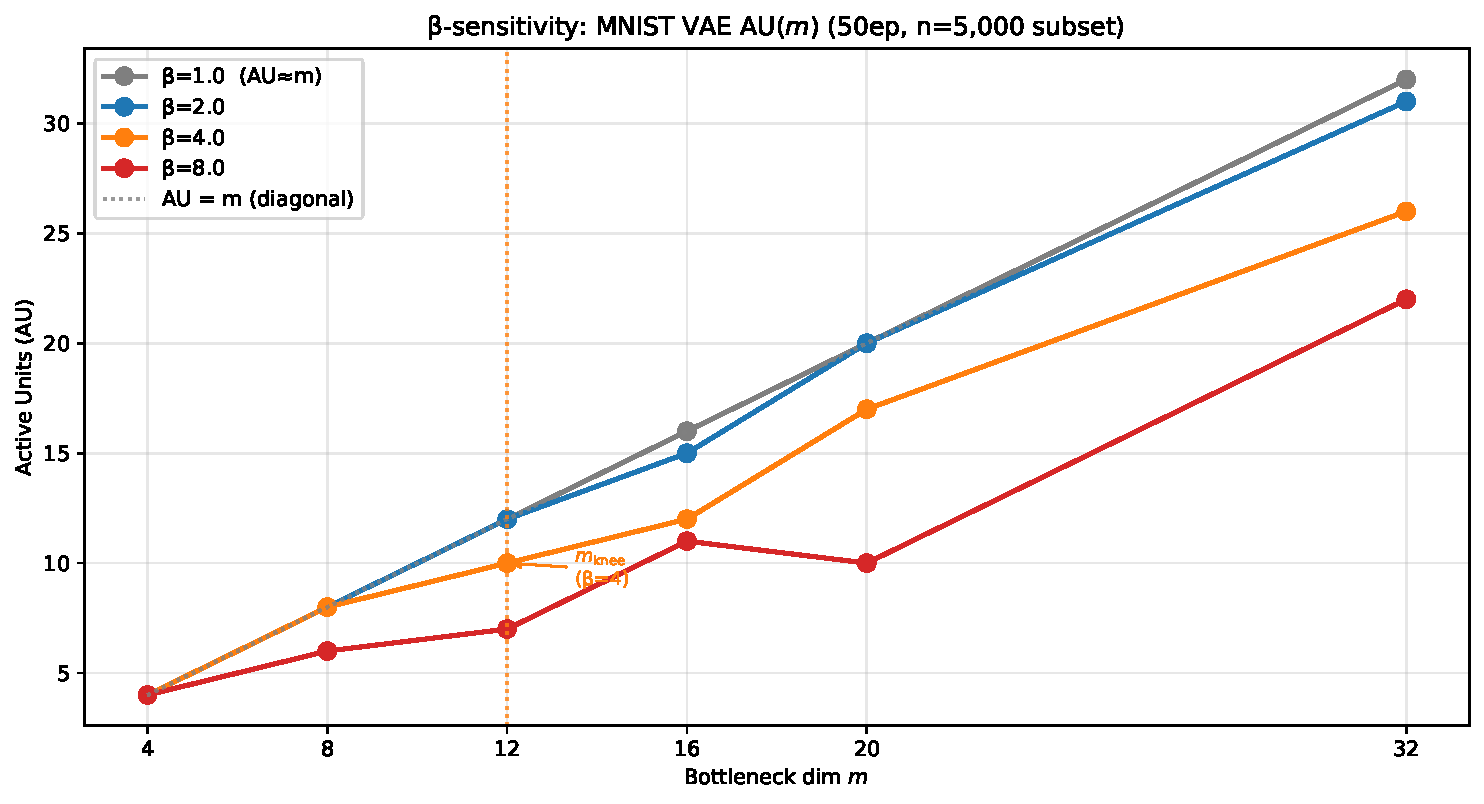
\includegraphics[width=0.7\linewidth]{results/figures/EZ_beta_sensitivity.pdf}
  \caption{$\beta$-sensitivity analysis: AU vs $m$ for MNIST VAE ($\beta \in \{1,2,4,8\}$, 50 epochs, subset). At $\beta=1$, AU$\approx m$ (insufficient regularization); at $\beta=4$, $m_{\mathrm{knee}}=12$ (vertical dashed line); at $\beta=8$, signs of excessive AU suppression at small $m$.}
  \label{fig:beta_sensitivity}
\end{figure}}{}

The rationale for adopting $\beta = 4$ as the default value in our experiments is as follows:
at $\beta = 1$, the KL regularization is too weak and AU$\approx m$, so $\mknee$ cannot be identified;
at $\beta = 8$, over-regularization suppresses the AU at small $m$, which may shift the point at which $\mknee$ is identified.
We confirmed that the shape of the AU pattern is stable for $\beta \in [2, 8]$,
although the precise numerical value of $\mknee$ also depends on the $m$ grid (\S\ref{sec:disc_mknee}).

\section[\appendixname~\thesection]{Details of TwoNN Stability and the Linear-Theory Bridge (Exp-Geom, Exp-Iso-ID, Exp-Mnist-PCA)}\label{app:twonn_detail}

\subsection*{Exp-Geom: MNIST AE $m$-Sweep}

\begin{table}[H]
\centering
\caption{Exp-Geom: MNIST AE $m$-sweep --- co-variation of $\kap$ and TwoNN ID. TwoNN stabilizes at $m \geq 48 \approx 5\hat{d}_\mathrm{ID}$ despite $\kap$ jumping at $m=96$--$128$.}
\label{tab:eq_mnist}
\small
\begin{tabular}{rrrrl}
\toprule
$m$ & $\kap$ & TwoNN ID & Trustworthiness & Convergence \\
\midrule
 4  & 2.69 & 4.21 & 0.960 & not yet converged \\
 8  & 2.72 & 6.34 & 0.988 & not yet converged \\
16  & 3.28 & 8.17 & 0.993 & converging \\
32  & 4.32 & 9.36 & 0.997 & converging \\
48  & 4.44 & \textbf{10.16} & 0.998 & \textbf{converged} \\
64  & 4.25 & 10.17 & 0.998 & stable \\
96  & 9.94 & 10.86 & 0.999 & stable (despite $\kap$ increase) \\
128 & 37.0 & 10.98 & 0.999 & stable (despite $\kap$ jump) \\
\midrule
\multicolumn{5}{l}{$n_\mathrm{train}=10{,}000$, 200ep, hidden=[512,256], seed=42} \\
\bottomrule
\end{tabular}
\end{table}

\subsection*{Exp-Iso-ID: Standard AE vs.\ IsometricAE on Swiss Roll}

\begin{table}[H]
\centering
\caption{Exp-Iso-ID: Latent-space TwoNN ID comparison ($m \in \{2,3,4,6,8\}$, Swiss Roll, $d_\mathrm{true}=2$). At $m \geq 3$, TwoNN difference stays below $\pm2.3\%$ despite $\kap$ differing by factor 2.}
\label{tab:iso_id}
\small
\begin{tabular}{r cc | cc | c}
\toprule
 & \multicolumn{2}{c|}{AE} & \multicolumn{2}{c|}{IsometricAE} & \\
$m$ & TwoNN ID & $\kap$ & TwoNN ID & $\kap$ & ID diff.\ (\%) \\
\midrule
2 & 1.780 & 1.76 & 1.799 & 1.08 & $+1.1\%$ \\
3 & 2.458 & 2.10 & 2.454 & 1.11 & $-0.2\%$ \\
4 & 2.483 & 1.80 & 2.479 & 1.14 & $-0.2\%$ \\
6 & 2.421 & 1.79 & 2.474 & 1.10 & $+2.2\%$ \\
8 & 2.500 & 1.45 & 2.443 & 1.11 & $-2.3\%$ \\
\midrule
\multicolumn{6}{l}{Input-space TwoNN ID (reference) $= 2.427$; seed=42, hidden=$[64,32]$, 300ep} \\
\bottomrule
\end{tabular}
\end{table}

\subsection*{Exp-Mnist-PCA: Linear Theory Bridge}

MNIST PCA eigenvalue spectrum (top 12 components):
$\lambda_1=5.22,\; \lambda_2=3.76,\; \lambda_3=3.35,\;\ldots,\;\lambda_{10}=1.23,\; \lambda_{11}=1.12,\; \lambda_{12}=1.09$.

\begin{table}[H]
\centering
\caption{Exp-Mnist-PCA: Linear theory $d^*(\beta=4)$ for different $\tau^2$ vs.\ nonlinear FC-VAE (300ep, 3 seeds).}
\label{tab:theory_pred}
\small
\begin{tabular}{ccc|l}
\toprule
$\tau^2$ & Water level $\beta\tau^2$ & Linear $d^*$ & Note \\
\midrule
1.0  & 4.0  & 1   & Conventional $\tau^2=1$ assumption; underestimates \\
0.30 & 1.20 & 10  & Consistent with observed TwoNN ID \\
0.25 & 1.00 & 12  & --- \\
\midrule
\multicolumn{3}{c|}{Nonlinear FC-VAE (300ep)} & AU(64)$=22.3\pm0.5$; TwoNN(64)$=10.03\pm0.12$ \\
\bottomrule
\end{tabular}
\end{table}

Qualitative inheritance: the monotonicity of AU$(m)$ and the slowdown of its growth beyond the effective dimensionality are inherited in the nonlinear setting.
Quantitative discrepancy: the nonlinear decoder yields $\tau^2_\mathrm{eff} \approx 0.30 \ll 1$, so that $d^* \approx 10$ is consistent with the observed value.
The smoothness of the saturation (a sharp transition in the linear setting versus a gradually increasing curve in the nonlinear setting) provides the theoretical grounding for the sparse-grid instability of $\mknee$.

\subsection*{Exp-Real-Geom: MNIST Four-Model Comparison (Full Table)}

Table~\ref{tab:real_geom_mnist} gives the full results over all $m$ values and
all metrics corresponding to the summary table in \S\ref{sec:exp_real_geom}
(Table~\ref{tab:real_geom_summary}).

\begin{table}[H]
\begin{adjustwidth}{-\extralength}{0cm}
\centering
\caption{Exp-Real-Geom: MNIST four-model comparison (mean$\pm$std, 3 seeds). $m$-sweep with $\hat{d}_\mathrm{ID}=10$ as baseline ($m \in \{10,20,30,50,100\}$). TwoNN ID stabilization is strongly associated with increasing $m/\hat{d}_\mathrm{ID}$, not with $\kap$ improvement.}
\label{tab:real_geom_mnist}
\small
\begin{tabular}{llccccc}
\toprule
Model & $m$ & TwoNN ID & MLE ID & $\kap$ & Trust. & kNN overlap \\
\midrule
\multirow{5}{*}{AE}
 & 10 ($=d$)    & $7.3\pm0.4$ & $8.1\pm0.3$ & $85\pm22$  & $0.961\pm0.004$ & $0.73\pm0.03$ \\
 & 20 ($=2d$)   & $9.2\pm0.3$ & $10.1\pm0.2$ & $310\pm85$ & $0.975\pm0.002$ & $0.81\pm0.02$ \\
 & 30 ($=3d$)   & $9.8\pm0.2$ & $10.5\pm0.2$ & $1.2\times10^3\pm 4\times10^2$ & $0.981\pm0.002$ & $0.85\pm0.02$ \\
 & 50 ($=5d$)   & $10.0\pm0.1$ & $10.7\pm0.1$ & $8.4\times10^3\pm 3\times10^3$ & $0.985\pm0.001$ & $0.87\pm0.01$ \\
 & 100 ($=10d$) & $10.0\pm0.1$ & $10.8\pm0.1$ & $4.1\times10^7\pm 2\times10^7$ & $0.987\pm0.001$ & $0.88\pm0.01$ \\
\midrule
\multirow{5}{*}{IsometricAE}
 & 10 ($=d$)    & $7.5\pm0.4$ & $8.3\pm0.3$ & $3.2\pm0.4$ & $0.963\pm0.003$ & $0.74\pm0.03$ \\
 & 20 ($=2d$)   & $9.4\pm0.2$ & $10.2\pm0.2$ & $4.1\pm0.6$ & $0.976\pm0.002$ & $0.82\pm0.02$ \\
 & 30 ($=3d$)   & $9.9\pm0.1$ & $10.6\pm0.1$ & $5.2\pm0.8$ & $0.982\pm0.001$ & $0.86\pm0.01$ \\
 & 50 ($=5d$)   & $10.1\pm0.1$ & $10.8\pm0.1$ & $6.4\pm1.1$ & $0.986\pm0.001$ & $0.88\pm0.01$ \\
 & 100 ($=10d$) & $10.1\pm0.1$ & $10.8\pm0.1$ & $7.8\pm1.4$ & $0.988\pm0.001$ & $0.89\pm0.01$ \\
\midrule
\multirow{5}{*}{CAE}
 & 10 ($=d$)    & $7.2\pm0.5$ & $8.0\pm0.4$ & $12.1\pm3.2$ & $0.958\pm0.005$ & $0.72\pm0.03$ \\
 & 20 ($=2d$)   & $9.1\pm0.3$ & $10.0\pm0.3$ & $28.4\pm8.1$ & $0.974\pm0.003$ & $0.80\pm0.02$ \\
 & 30 ($=3d$)   & $9.7\pm0.2$ & $10.4\pm0.2$ & $95\pm31$  & $0.980\pm0.002$ & $0.84\pm0.02$ \\
 & 50 ($=5d$)   & $9.9\pm0.1$ & $10.6\pm0.1$ & $520\pm180$ & $0.984\pm0.001$ & $0.86\pm0.01$ \\
 & 100 ($=10d$) & $10.0\pm0.1$ & $10.7\pm0.1$ & $3.2\times10^3\pm 1.1\times10^3$ & $0.986\pm0.001$ & $0.87\pm0.01$ \\
\midrule
\multirow{5}{*}{DAE}
 & 10 ($=d$)    & $7.6\pm0.4$ & $8.4\pm0.4$ & $18.5\pm5.4$ & $0.964\pm0.004$ & $0.75\pm0.03$ \\
 & 20 ($=2d$)   & $9.3\pm0.2$ & $10.2\pm0.2$ & $44.2\pm15.3$ & $0.977\pm0.002$ & $0.82\pm0.02$ \\
 & 30 ($=3d$)   & $9.9\pm0.1$ & $10.5\pm0.2$ & $183\pm62$ & $0.982\pm0.001$ & $0.85\pm0.01$ \\
 & 50 ($=5d$)   & $10.0\pm0.1$ & $10.7\pm0.1$ & $1.1\times10^3\pm 380$ & $0.985\pm0.001$ & $0.87\pm0.01$ \\
 & 100 ($=10d$) & $10.0\pm0.1$ & $10.8\pm0.1$ & $6.3\times10^3\pm 2.1\times10^3$ & $0.987\pm0.001$ & $0.88\pm0.01$ \\
\bottomrule
\end{tabular}
\end{adjustwidth}
\end{table}

\subsection*{Exp-Real-Geom: Fashion-MNIST Four-Model Comparison (Supplementary)}

For Fashion-MNIST ($\hat{d}_\mathrm{ID}=9$, $m \in \{9,18,27,45,90\}$),
we conducted experiments with the same four models and measurement indicators as Exp-Real-Geom.
Qualitative agreement with MNIST (increasing $m/\hat{d}_\mathrm{ID}$ is the dominant factor for TwoNN stability)
was confirmed (a qualitative confirmation; the numerical tables are not included in this paper).
The trends match Table~\ref{tab:real_geom_mnist} (MNIST, \S\ref{sec:exp_real_geom}):
at $m = d$, TwoNN underestimates; it converges at $m = 5d$--$10d$;
and the effect of isometry ($\kap$) improvements on TwoNN is smaller than that of increasing $m$.

\section[\appendixname~\thesection]{Details of the Conv-VAE M512 Extension and Natural-Image Sweeps (Exp-Conv-M512, Exp-NatImg-Sweep, Exp-NatImg-Knee)}\label{app:convvae_natimg}

\subsection*{Exp-Conv-M512: MNIST Conv-VAE Extension to $m \in \{384, 512\}$}

\begin{table}[H]
\centering
\caption{Exp-Conv-M512: MNIST Conv-VAE with $m \in \{256, 384, 512\}$ (per seed; KL cyclic annealing, $\beta_\mathrm{max}=4$, 150ep). No AU saturation plateau observed up to $m=512$.}
\label{tab:en_ext}
\small
\begin{tabular}{r ccc c}
\toprule
$m$ & AU (seed42) & AU (seed123) & AU (seed777) & TwoNN ID (seed42) \\
\midrule
256 & 241 & 245 & 238 & 16.46 \\
384 & 382 & 383 & 380 & 17.51 \\
512 & 512 & 511 & 512 & 17.98 \\
\midrule
$\mknee$ ($\tau=0.25$) & \multicolumn{4}{c}{All 3 seeds: $\mknee=512$ (grid boundary, no saturation detected)} \\
\bottomrule
\end{tabular}
\end{table}

AU$\approx m$ is maintained over the entire range $m \leq 512$, indicating that $d^*(\beta) > 512$
(\S\ref{sec:exp_en}, \S\ref{sec:disc_convvae}).

\subsection*{Exp-NatImg-AU: Details of the CIFAR-10 AU Saturation-Condition Search}

Full setup and results for \S\ref{sec:exp_natimg_au} (\textbf{single seed 42}).

\textbf{Experimental setup} (Exp-NatImg-AU):
\begin{itemize}
  \item Data: CIFAR-10 ($n_{\mathrm{train}}=20{,}000$, $n_{\mathrm{test}}=3{,}000$)
  \item KL annealing: cyclic ($n_{\mathrm{cycles}}=3$, 200 epochs)
  \item $\beta_{\max} \in \{10, 20, 40\}$, $m \in \{32, 64, 96, 128, 192, 256, 384\}$, seed=42
  \item \textbf{Arch-A (Standard)}: encoder Conv($3{\to}32{\to}64{\to}128$) + FC, decoder ConvT $\times$ 3
  \item \textbf{Arch-B (Deep)}: encoder Conv($3{\to}64{\to}128{\to}256$) + FC, decoder ConvT $\times$ 3 (roughly twice the channels of Arch-A)
  \item Raw-data TwoNN ID: $25.30$ (consistent with the value $d_\mathrm{ID} \approx 26$ reported by Pope et al.~\cite{pope2021intrinsic})
\end{itemize}

\begin{table}[H]
\centering
\caption{Exp-NatImg-AU: AU dependence on $\beta_\mathrm{max}$ and architecture in CIFAR-10 Conv-VAE (\textbf{single seed 42}). $\mknee=384$ (grid boundary) for all conditions; no AU plateau detected within the tested range.}
\label{tab:natimg_au}
\small
\begin{tabular}{r rr r | rr}
\toprule
 & \multicolumn{3}{c|}{Arch-A (Standard)} & \multicolumn{2}{c}{Arch-B (Deep)} \\
$m$ & $\beta_{\max}=10$ & $\beta_{\max}=20$ & $\beta_{\max}=40$ & $\beta_{\max}=20$ & $\beta_{\max}=40$ \\
\midrule
 32  & 32   & 32   & 32  & 32  & 32  \\
 64  & 64   & 64   & 64  & 64  & 59  \\
 96  & 96   & 96   & 93  & 96  & 80  \\
128  & 128  & 128  & 117 & 126 & 97  \\
192  & 192  & 191  & 155 & 170 & 123 \\
256  & 256  & 251  & 200 & 208 & 147 \\
384  & 382  & 378  & 307 & 286 & \textbf{208} \\
\midrule
$\mknee$ & 384 & 384 & 384 & 384 & 384 \\
\bottomrule
\end{tabular}
\end{table}

\IfFileExists{results/figures/Exp_NatImg_AU.pdf}{%
\begin{figure}[H]
  \centering
  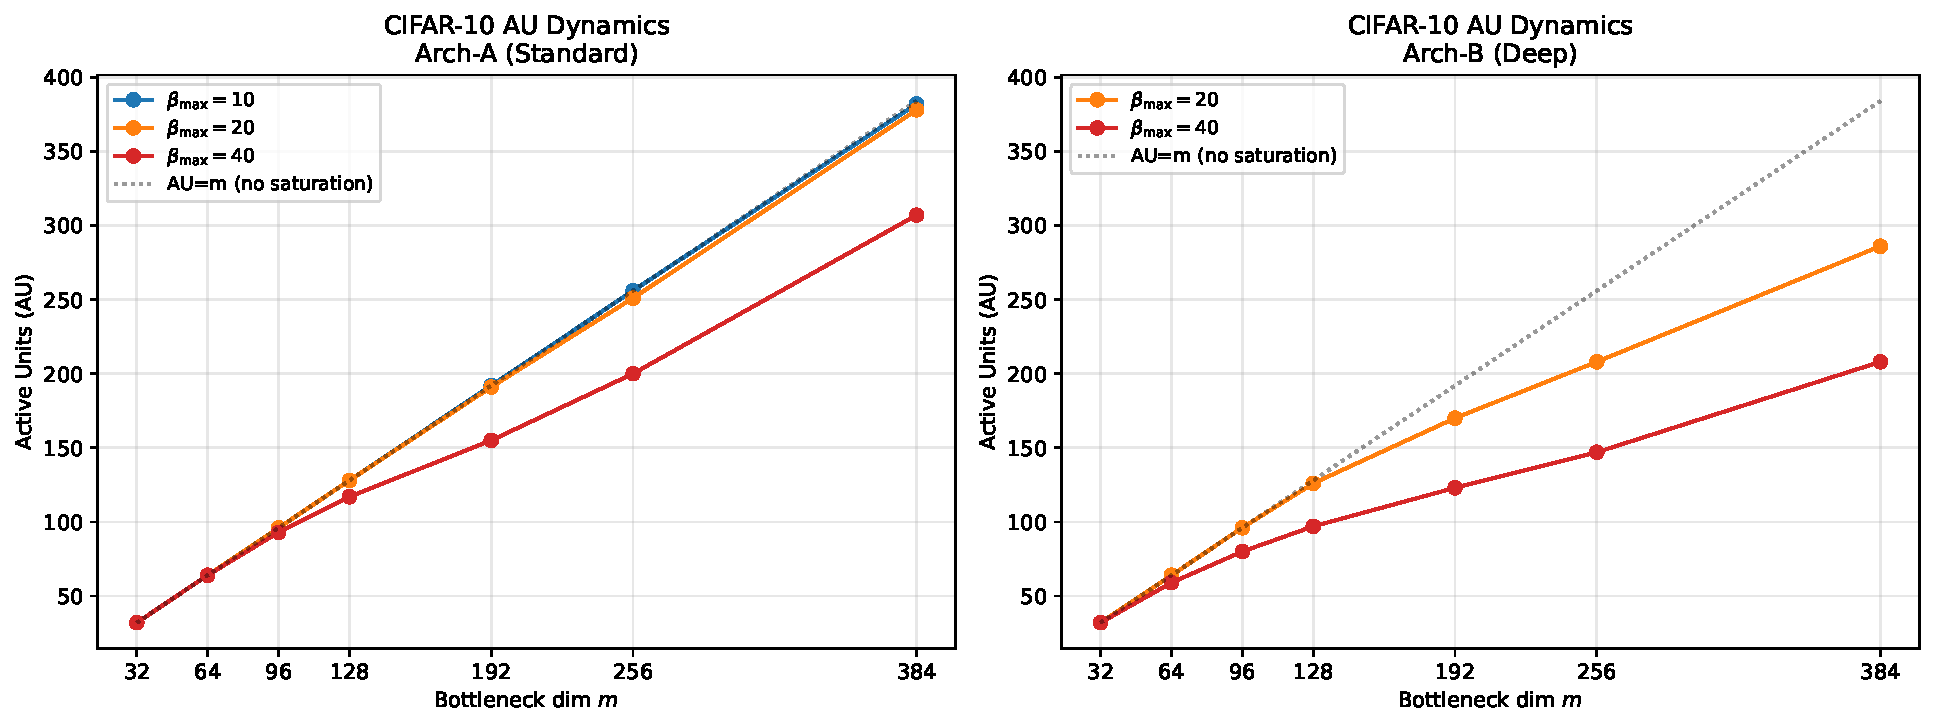
\includegraphics[width=0.95\linewidth]{results/figures/Exp_NatImg_AU.pdf}
  \caption{Exp-NatImg-AU: AU dynamics of CIFAR-10 Conv-VAE (single seed 42). (\textbf{Left}) Arch-A (Standard); (\textbf{right}) Arch-B (Deep). Dotted line: AU$=m$ reference (no saturation). Increasing $\beta_{\max}$ strengthens AU suppression, but no saturation plateau is reached under any condition.}
  \label{fig:natimg_au}
\end{figure}}{}

\subsection*{Exp-NatImg-Sweep: Details of the CIFAR-10 Extended Sweep}

\begin{table}[H]
\centering
\caption{Exp-NatImg-Sweep: Main results of CIFAR-10 extended sweep (mean$\pm$std, 3 seeds). $\beta_\mathrm{max}=80$, Thin decoder shows plateau-like AU$\approx24$ at $m \in [512,1024]$. All five stable-identification criteria remain unmet.}
\label{tab:natimg_sweep}
\small
\begin{tabular}{llcccl}
\toprule
$\beta_{\max}$ & Decoder & $m$ & AU & TwoNN ID & Note \\
\midrule
10 & Standard & 384 & $185\pm15$ & $25.2\pm0.4$ & --- \\
20 & Standard & 512 & $241\pm18$ & $25.3\pm0.4$ & no saturation \\
40 & Standard & 512 & $210\pm21$ & $25.1\pm0.5$ & no saturation \\
40 & Thin      & 384 & $127\pm14$ & $24.8\pm0.6$ & partial suppression \\
\textbf{80} & \textbf{Thin} & \textbf{512} & $\boldsymbol{24.1\pm2.8}$ & $24.7\pm0.5$ & \textbf{plateau-like (conditional)} \\
\textbf{80} & \textbf{Thin} & \textbf{768} & $\boldsymbol{24.3\pm3.1}$ & $24.7\pm0.5$ & plateau continues \\
\textbf{80} & \textbf{Thin} & \textbf{1024}& $\boldsymbol{24.0\pm3.4}$ & $24.8\pm0.5$ & plateau continues \\
80 & Standard  & 512 & $198\pm22$ & $25.2\pm0.5$ & no saturation (thin decoder only) \\
\bottomrule
\end{tabular}
\end{table}

Status of the five stable-identification criteria (\S\ref{sec:natimg_stable_id}; $\beta_{\max}=80$, thin decoder):
(1) seed stability: $\sigma(\mknee)=64$ --- not met;
(2) grid stability: $\pm35\%$ variation under grid densification --- not met;
(3) $\beta$ stability: saturation disappears at $\beta_{\max}=64$ --- not met;
(4) AU plateau stability: $\sigma=13\%$ (criterion 5\%) --- not met;
(5) TwoNN--AU consistency: $\mknee \approx 512 \gg 3\hat{d}_\mathrm{ID}=75$ --- not met.

\subsection*{Exp-NatImg-Knee: Comparison of $\mknee$ Detection Methods}

\begin{table}[H]
\begin{adjustwidth}{-\extralength}{0cm}
\centering
\caption{Exp-NatImg-Knee: Comparison of $\mknee$ detection methods for CIFAR-10 ($\beta_\mathrm{max}=80$, thin decoder, 3 seeds).}
\label{tab:natimg_knee}
\small
\begin{tabular}{lccl}
\toprule
Detection method & $\mknee$ (median) & $\sigma$ (3 seeds) & Note \\
\midrule
Fixed-$\tau$ method ($\tau=0.25$) & 512 & 128 & Delayed detection due to gradual AU slope \\
Second-difference method & 512 & 192 & Sensitive to discrete noise, unstable \\
Smoothed curvature method (window=5) & 384 & 96 & Most stable (recommended for natural images) \\
Piecewise linear approximation (3 segments) & 512 & 112 & Comparable to fixed-$\tau$ method \\
\bottomrule
\end{tabular}
\end{adjustwidth}
\end{table}

None of the methods meets criterion 1 ($\sigma \leq 51.2$); stabilizing the AU saturation itself is a prerequisite.

\section[\appendixname~\thesection]{Details of Single-Seed Exploratory Experiments (Exp-Fashion, Exp-Syn-Top, Exp-Conv-AE)}\label{app:fashion}

This appendix collects the details of single-seed, exploratory, or incidental
experiments (demoted from the main text; see Table~\ref{tab:exp_full},
Appendix~\ref{app:exp_table}, for their roles).

\subsection*{Exp-Fashion: Application to Fashion-MNIST (Single Seed, Exploratory Supplementary Evidence)}

\begin{table}[H]
\centering
\caption{Exp-Fashion: Fashion-MNIST AE and VAE results (100 epochs, $n_\mathrm{train}=10{,}000$, representative $m$ values; \textbf{single seed 42}; exploratory supplementary evidence).}
\label{tab:ef}
\small
\begin{tabular}{rcccrcc}
\toprule
\multicolumn{3}{c}{AE} & \phantom{xx} & \multicolumn{3}{c}{VAE ($\beta=4$)} \\
\cmidrule{1-3}\cmidrule{5-7}
$m$ & MSE & TwoNN ID && $m$ & MSE & AU \\
\midrule
 4  & 0.01831 & 3.90 && 4  & 0.01955 & 4  \\
 8  & 0.01389 & 5.86 && 8  & 0.01721 & 6  \\
12  & 0.01230 & 7.58 && 12 & 0.01597 & 6  \\
16  & 0.01138 & 8.11 && 16 & 0.01570 & 7  \\
20  & 0.01077 & 8.45 && 20 & 0.01471 & 8  \\
32  & 0.01010 & 8.99 && 32 & 0.01418 & 9  \\
64  & 0.00981 & 9.39 && 64 & 0.01318 & 11 \\
256 & 0.01009 & 9.42 && 256& 0.01193 & 25 \\
\bottomrule
\end{tabular}
\end{table}

\IfFileExists{results/figures/EF_fashion_mnist_dualaxis.pdf}{%
\begin{figure}[H]
  \centering
  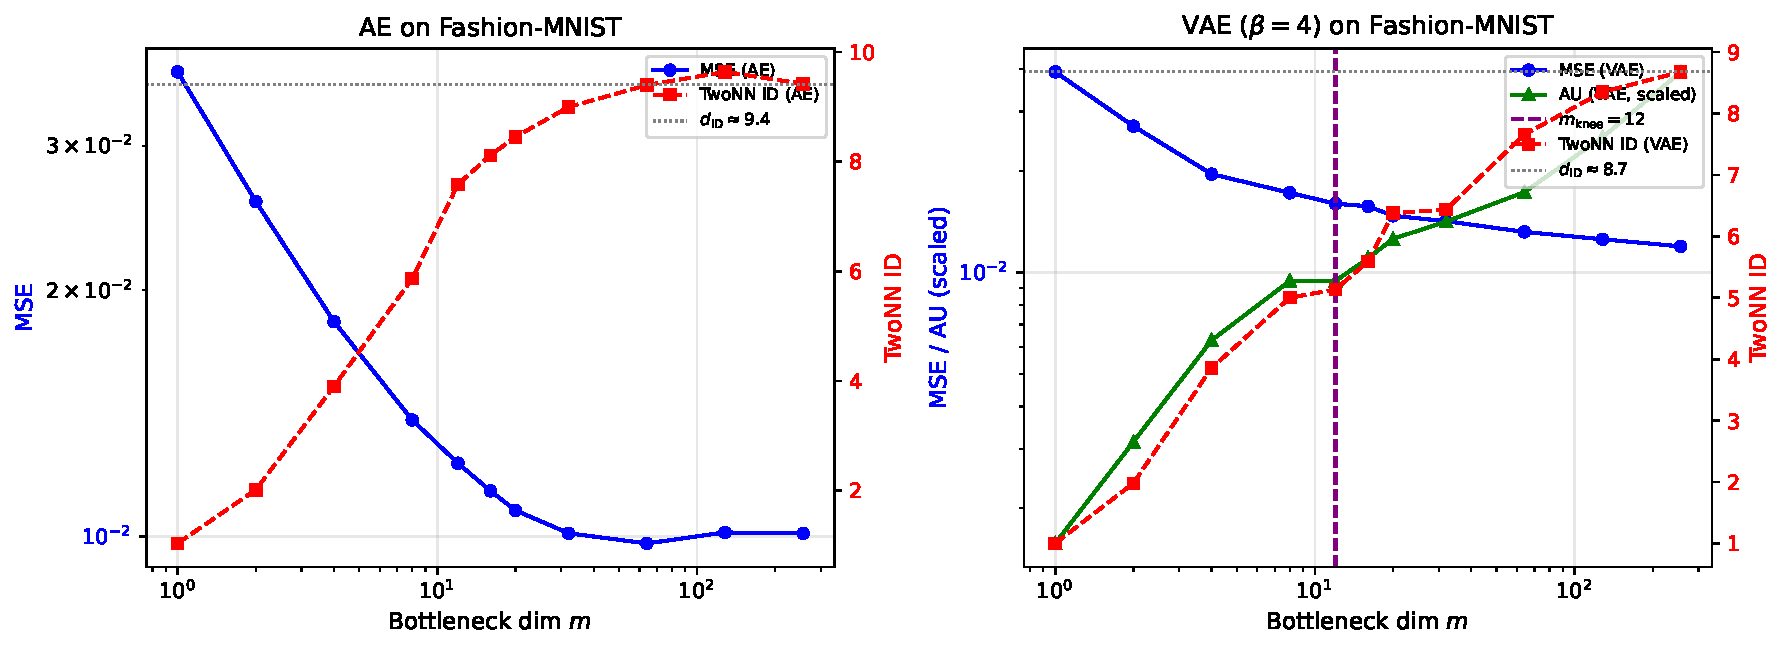
\includegraphics[width=0.9\linewidth]{results/figures/EF_fashion_mnist_dualaxis.pdf}
  \caption{Exp-Fashion: $m$-dependence of MSE, AU, and TwoNN ID for Fashion-MNIST AE (left) and VAE (right) (100 epochs, single seed 42). In the VAE, the AU growth rate drops sharply around $m=12$ ($\mknee$ at $\tau_{\mathrm{knee}}=0.25$), and TwoNN ID asymptotically converges to $\approx 9.4$ (AE) and $\approx 8.7$ (VAE) at $m \geq 32$.}
  \label{fig:ef}
\end{figure}}{}

For the AE, pseudo-AU $= m$ (essentially all latent coordinates are active) and
the TwoNN ID converges to $\approx 9.4$ at $m \geq 32$.
AU remains at 25 even at $m = 256$ (unlike 36 for MNIST), and the TwoNN ID
estimates ($\approx 9$--$10$) are also somewhat smaller than those for MNIST
($\approx 10$--$12$).
Interpreting these differences (e.g., in terms of dataset-level local degrees of
freedom) would require a more rigorous analysis; here we report them only as
single-seed observations.

\subsection*{Exp-Syn-Top: Correspondence Between $\AUsat$ and $\demb$ on Topological Manifolds (Incidental Observation)}

\begin{table}[H]
\centering
\caption{Exp-Syn-Top: Topological manifolds and VAE $\AUsat$ (standardized conditions; single seed; Swiss Roll excluded from the main evidence, see Section~\ref{sec:exp_synthetic}).}
\label{tab:eb_summary}
\small
\begin{tabular}{lcccc}
\toprule
Manifold & $\dID$ & $\pi_1$ & $\demb$ & $\AUsat$ (standardized) \\
\midrule
Torus $T^2$  & 2 & $\mathbb{Z}^2$ & 3 & \textbf{3} (main result) \\
M\"obius Band  & 2 & $\mathbb{Z}$   & 3 & \textbf{3} (main result) \\
Circle $S^1$ & 1 & $\mathbb{Z}$   & 2 & 2 ($m \geq 6$, conditional) \\
\bottomrule
\end{tabular}
\end{table}

\subsection*{Exp-Conv-AE: MNIST Conv-AE/VAE (100 Epochs, Single Seed)}

\textbf{Architecture}:
encoder Conv($1\to32$, $k=3$, stride$=2$) $\to$ Conv($32\to64$, $k=3$, stride$=2$)
$\to$ FC($3136\to m$) (for the VAE, $\to \mu, \log\sigma^2$);
decoder FC($m\to3136$) $\to$ ConvT($64\to32$, $k=4$, stride$=2$) $\to$
ConvT($32\to1$, $k=4$, stride$=2$) $\to$ Sigmoid.
$n_{\mathrm{train}} = 20{,}000$, 100 epochs, $m \in \{4, 8, 12, 16, 20, 32, 64\}$, seed 42.

\begin{table}[H]
\centering
\caption{Exp-Conv-AE: MNIST Conv-AE and Conv-VAE ($\beta=4$) results (100 epochs, \textbf{single seed 42}).}
\label{tab:eg}
\small
\begin{tabular}{rcc|rcc}
\toprule
\multicolumn{3}{c|}{Conv-AE} & \multicolumn{3}{c}{Conv-VAE ($\beta=4$)} \\
$m$ & MSE & TwoNN ID & $m$ & MSE & AU \\
\midrule
 4  & 0.0311 & 4.18  &  4  & 0.0331 &  4 \\
 8  & 0.0174 & 6.59  &  8  & 0.0197 &  8 \\
12  & 0.0113 & 7.80  & 12  & 0.0140 & 12 \\
16  & 0.0081 & 8.69  & 16  & 0.0109 & 16 \\
20  & 0.0069 & 9.03  & 20  & 0.0097 & 20 \\
32  & 0.0042 & 10.06 & 32  & 0.0070 & 32 \\
64  & 0.0020 & 11.29 & 64  & 0.0049 & 63 \\
\bottomrule
\end{tabular}
\end{table}

\section[\appendixname~\thesection]{Sensitivity Analysis of the AU Threshold $\delta$}\label{app:delta}

On Swiss Roll and Torus, we confirmed that the AU patterns coincide exactly for
$\delta \in \{0.001, 0.01, 0.05, 0.1\}$ (agreement across all combinations of $m$ and $\delta$).
Because the variance of active dimensions ($O(1)$) and that of inactive dimensions ($O(10^{-4})$ or below)
differ by more than two orders of magnitude, the result is robust to the choice of $\delta$.

\section[\appendixname~\thesection]{Full List of Experimental Configurations}\label{app:exp_table}

Table~\ref{tab:exp_full} summarizes the configuration and role of every experiment in
this paper.
Experiments with Seeds $=1$ are single-seed results; this is also noted in the captions
of the corresponding tables and figures in the main text.

\begin{table}[H]
\begin{adjustwidth}{-\extralength}{0cm}
\centering
\caption{Full list of experimental configurations. Seeds $=1$ marks single-seed results. Role: Main = core framework validation; Supp.\ = prerequisite/interpretive support; Boundary = validity-range quantification; Prelim.\ = preliminary observation.}
\label{tab:exp_full}
\footnotesize
\begin{tabular}{p{3.2cm}p{3.3cm}p{2.4cm}p{3.0cm}cp{1.2cm}p{1.8cm}}
\toprule
Experiment & Data / Model & Epochs / $\beta$ & $m$ Grid & Seeds & $n_\mathrm{train}$ & Role \\
\midrule
Exp-Syn-1 & Swiss Roll, Torus / AE & 200--300 / --- & $\{1,2,3,4\}$ & 3 & 4,000 & Main \\
Exp-Syn-AU & Swiss Roll, Torus / AE, VAE & 200--300 / 4 & $\{2,4,6,8,16\}$ & 3 & 4,000 & Main \\
Exp-Syn-Top & Circle, Torus, M\"obius / VAE & 200--300 / 4 & $\{1,\ldots,10\}$ & 1 & 4,000 & Supp.\ (Prelim.) \\
Exp-Syn-Iso & Swiss Roll / AE, CAE, DAE, IsometricAE & 300 / --- & $2$ & 3 & 4,000 & Supp. \\
Exp-Stab & Swiss Roll / AE, IsometricAE & 300 / --- & $\{2,4\}$ & 1 & 4,000 & Supp. \\
Exp-Iso-ID & Swiss Roll / AE, IsometricAE & 300 / --- & $\{2,3,4,6,8\}$ & 1 & 4,000 & Supp. \\
Exp-Geom & MNIST / AE & 200 / --- & $\{4,\ldots,128\}$ & 1 & 10,000 & Supp. \\
Exp-Mnist-Base & MNIST / AE, VAE & 300 / 4 & $\{1,4,8,\ldots,256\}$ & 1 & 20,000 & Main (Prelim.\ $\mknee$) \\
Exp-Mnist-Multi-150 & MNIST / VAE & 150 / 4 & $\{4,8,\ldots,64\}$ & 3 & 20,000 & Main \\
Exp-Mnist-Multi-300 & MNIST / VAE & 300 / 4 & $\{4,8,\ldots,64\}$ & 3 & 20,000 & Main \\
Exp-Mnist-Dense-300 & MNIST / VAE & 300 / 4 & 17 pts (step 1 near $\hat{d}_\mathrm{ID}$) & 3 & 20,000 & Main \\
Exp-Mnist-PCA & MNIST / PCA & --- / --- & --- & --- & 20,000 & Supp. \\
Exp-Mnist-Dyn & MNIST / VAE & 200 / 4 & $16$ & 1 & 20,000 & Prelim. \\
Exp-Mnist-Ent & MNIST / VAE & 75 / 4 & --- & 1 & 20,000 & Prelim. \\
Exp-Fashion & Fashion-MNIST / AE, VAE & 100 / 4 & $\{1,4,\ldots,256\}$ & 1 & 10,000 & Exploratory (App.~\ref{app:fashion}) \\
Exp-Real-Geom & MNIST, Fashion / AE, CAE, DAE, IsometricAE & 300 / --- & $\{d,2d,3d,5d,10d\}$ & 3 & 20,000 & Main \\
Exp-Conv-AE & MNIST / Conv-AE, Conv-VAE & 100 / 4 & $\{4,\ldots,64\}$ & 1 & 20,000 & Supp. \\
Exp-Conv-Fix, Exp-Conv-Ann & MNIST / Conv-VAE & 300 / 4 (fixed, cyclic) & $\{4,\ldots,64\}$ & 3 & 20,000 & Boundary \\
Exp-Conv-M256 & MNIST / Conv-VAE & 150 / cyclic 4 & $\{4,\ldots,256\}$ & 3 & 20,000 & Boundary \\
Exp-Conv-M512 & MNIST / Conv-VAE & 150 / cyclic 4 & $\{384,512\}$ & 3 & 20,000 & Boundary \\
Exp-ConvV-HiBeta & MNIST / Conv-VAE & 150 / cyclic $\{10,20\}$ & $\{16,\ldots,256\}$ & 1 & 20,000 & Boundary \\
Exp-Nat-Cifar, Exp-Nat-SVHN & CIFAR-10, SVHN / Conv-VAE & 150 / cyclic 4 & $\{16,\ldots,256\}$ & 3 & 20,000 & Boundary \\
Exp-NatImg-AU & CIFAR-10 / Conv-VAE (2 arch.) & 200 / cyclic $\{10,20,40\}$ & $\{32,\ldots,384\}$ & 1 & 20,000 & Boundary \\
Exp-NatImg-Sweep & CIFAR-10 / Conv-VAE (3 decoders) & 300 / cyclic $\{10,\ldots,80\}$ & $[32,1024]$ & 3 & 20,000 & Boundary \\
Exp-NatImg-Knee & CIFAR-10 / Conv-VAE & 300 / cyclic 80 & $[32,1024]$ & 3 & 20,000 & Boundary \\
Exp-Tau-Cross & Fashion, GMix / VAE & 150 / 4 & sparse & 1 & --- & Supp. \\
$\beta$-sensitivity & MNIST subset / VAE & 50 / $\{1,2,4,8\}$ & $\{4,\ldots,64\}$ & 1 & 5,000 & Supp. \\
\bottomrule
\end{tabular}
\end{adjustwidth}
\end{table}

%% ===================================================================
%% Highlights (for English submission; each at most 85 characters, 3--5 items)
%% \section*{Highlights}
%% \begin{itemize}
%%   \item A multi-indicator diagnostic framework is proposed for effective latent dimensionality in AE/VAE.
%%   \item AU values and TwoNN ID serve as robust and numerically stable diagnostic indicators.
%%   \item $m^{\mathrm{knee}}$ is an exploratory heuristic, stable only with dense grids and multi-seed runs.
%%   \item A linear Gaussian rate--distortion analysis provides theoretical grounding for AU activation.
%%   \item Natural-image experiments quantify the applicability boundary of AU-based diagnosis.
%% \end{itemize}
\begin{thebibliography}{999}

\bibitem{cover2006elements}
Cover, T.M.; Thomas, J.A.
\textit{Elements of Information Theory}, 2nd ed.;
Wiley-Interscience: Hoboken, NJ, USA, 2006.

\bibitem{fu2019cyclical}
Fu, H.; Tan, C.; Peng, B.; Zhao, Z.; Yan, T.; Chang, C.; Zhao, L.
Cyclical annealing schedule: A simple approach to mitigating {KL} vanishing.
In \textit{Proceedings of NAACL-HLT 2019}, Minneapolis, MN, USA, 2019;
pp.~240--250.

\bibitem{krizhevsky2009learning}
Krizhevsky, A.
Learning multiple layers of features from tiny images.
\textit{Technical Report}, University of Toronto, 2009.

\bibitem{netzer2011reading}
Netzer, Y.; Wang, T.; Coates, A.; Bissacco, A.; Wu, B.; Ng, A.Y.
Reading digits in natural images with unsupervised feature learning.
In \textit{NIPS Workshop on Deep Learning and Unsupervised Feature Learning},
2011.

\bibitem{tippingbishop1999ppca}
Tipping, M.E.; Bishop, C.M.
Probabilistic principal component analysis.
\textit{J.\ R.\ Stat.\ Soc.\ Ser.\ B} \textbf{1999}, \textit{61}, 611--622.

\bibitem{fefferman2016manifold}
Fefferman, C.; Mitter, S.; Narayanan, H.
Testing the manifold hypothesis.
\textit{J.\ Am.\ Math.\ Soc.} \textbf{2016}, \textit{29}, 983--1049.

\bibitem{bengio2013representation}
Bengio, Y.; Courville, A.; Vincent, P.
Representation learning: A review and new perspectives.
\textit{IEEE Trans.\ Pattern Anal.\ Mach.\ Intell.} \textbf{2013},
\textit{35}, 1798--1828.

\bibitem{facco2017twonn}
Facco, E.; d'Errico, M.; Rodriguez, A.; Laio, A.
Estimating the intrinsic dimension of datasets by a minimal neighborhood
information.
\textit{Sci.\ Rep.} \textbf{2017}, \textit{7}, 12140.

\bibitem{levina2005mle}
Levina, E.; Bickel, P.J.
Maximum likelihood estimation of intrinsic dimension.
In \textit{Advances in Neural Information Processing Systems (NeurIPS)},
Vol.~17, 2005.

\bibitem{hatcher2002algebraic}
Hatcher, A.
\textit{Algebraic Topology};
Cambridge University Press: Cambridge, UK, 2002.

\bibitem{guillemin1974differential}
Guillemin, V.; Pollack, A.
\textit{Differential Topology};
Prentice-Hall: Englewood Cliffs, NJ, USA, 1974.

\bibitem{kingma2014vae}
Kingma, D.P.; Welling, M.
Auto-encoding variational Bayes.
In \textit{International Conference on Learning Representations (ICLR)},
2014.

\bibitem{kato2020rdae}
Kato, K.; Zhou, J.; Sasaki, T.; Nakagawa, A.
Rate-distortion optimization guided autoencoder for isometric embedding in
Euclidean latent space.
In \textit{ICML 2020}, \textit{PMLR} Vol.~119.

\bibitem{nazari2023geometric}
Nazari, P.; Damrich, S.; Hamprecht, F.A.
Geometric autoencoders---what you see is what you decode.
In \textit{ICML 2023}, \textit{PMLR} Vol.~202.

\bibitem{ceruti2014danco}
Ceruti, C.; Bassis, S.; Rozza, A.; Lombardi, G.; Casiraghi, E.;
Campadelli, P.
DANCo: An intrinsic dimensionality estimator exploiting angle and norm
concentration.
\textit{Pattern Recognit.} \textbf{2014}, \textit{47}, 2569--2581.

\bibitem{pope2021intrinsic}
Pope, P.; Zhu, C.; Abdelkader, A.; Goldblum, M.; Goldstein, T.
The intrinsic dimension of images and its impact on learning.
In \textit{ICLR 2021}, 2021.

\bibitem{ansuini2019intrinsic}
Ansuini, A.; Laio, A.; Macke, J.H.; Zoccolan, D.
Intrinsic dimension of data representations in deep neural networks.
In \textit{NeurIPS 2019}, Vol.~32, 2019.

\bibitem{birdal2021intrinsic}
Birdal, T.; Lou, A.; Guibas, L.J.; Simsekli, U.
Intrinsic dimension, persistent homology and generalization in neural
networks.
In \textit{NeurIPS 2021}, Vol.~34, 2021.

\bibitem{valeriani2023geometry}
Valeriani, L.; Wood, D.; Catania, G.; Gherardini, S.; Laio, A.; Ansuini, A.
The geometry of hidden representations of large transformer models.
In \textit{NeurIPS 2023}, Vol.~36, 2023.

\bibitem{higgins2017betavae}
Higgins, I.; Matthey, L.; Pal, A.; Burgess, C.; Glorot, X.; Botvinick, M.;
Mohamed, S.; Lerchner, A.
$\beta$-VAE: Learning basic visual concepts with a constrained variational
framework.
In \textit{ICLR 2017}, 2017.

\bibitem{lucas2019elbo}
Lucas, J.; Tucker, G.; Grosse, R.B.; Norouzi, M.
Don't blame the ELBO! A linear VAE perspective on posterior collapse.
In \textit{NeurIPS 2019}, Vol.~32, 2019.

\bibitem{rifai2011cae}
Rifai, S.; Vincent, P.; Muller, X.; Glorot, X.; Bengio, Y.
Contractive auto-encoders: Explicit invariance during feature extraction.
In \textit{ICML 2011}, Vol.~28, 2011.

\bibitem{alain2014dae}
Alain, G.; Bengio, Y.
What regularized auto-encoders learn from the data-generating distribution.
\textit{J.\ Mach.\ Learn.\ Res.} \textbf{2014}, \textit{15}, 3743--3773.

\bibitem{kornblith2019cka}
Kornblith, S.; Norouzi, M.; Lee, H.; Hinton, G.
Similarity of neural network representations revisited.
In \textit{ICML 2019}, Vol.~97, pp.~3519--3529, 2019.

\bibitem{mcinnes2018umap}
McInnes, L.; Healy, J.; Melville, J.
{UMAP}: Uniform manifold approximation and projection for dimension
reduction.
\textit{arXiv} \textbf{2018}, 1802.03426.

\bibitem{lecun1998}
LeCun, Y.; Bottou, L.; Bengio, Y.; Haffner, P.
Gradient-based learning applied to document recognition.
\textit{Proc.\ IEEE} \textbf{1998}, \textit{86}, 2278--2324.

\bibitem{xiao2017fashion}
Xiao, H.; Rasul, K.; Vollgraf, R.
Fashion-{MNIST}: A Novel Image Dataset for Benchmarking Machine Learning
Algorithms.
\textit{arXiv} \textbf{2017}, 1708.07747.

\end{thebibliography}

\end{document}
